\documentclass[a4paper]{article}

\def\npart {III}
\def\nterm {Lent}
\def\nyear {2017}
\def\nlecturer {C.\ E.\ Thomas}
\def\ncourse {The Standard Model}
\def\nofficial {https://www.damtp.cam.ac.uk/user/cet34/teaching/SM/}

% Imports
\ifx \nextra \undefined
  \usepackage[pdftex,
    hidelinks,
    pdfauthor={Dexter Chua},
    pdfsubject={Cambridge Maths Notes: Part \npart\ - \ncourse},
    pdftitle={Part \npart\ - \ncourse},
  pdfkeywords={Cambridge Mathematics Maths Math \npart\ \nterm\ \nyear\ \ncourse}]{hyperref}
  \title{Part \npart\ - \ncourse}
\else
  \usepackage[pdftex,
    hidelinks,
    pdfauthor={Dexter Chua},
    pdfsubject={Cambridge Maths Notes: Part \npart\ - \ncourse\ (\nextra)},
    pdftitle={Part \npart\ - \ncourse\ (\nextra)},
  pdfkeywords={Cambridge Mathematics Maths Math \npart\ \nterm\ \nyear\ \ncourse\ \nextra}]{hyperref}

  \title{Part \npart\ - \ncourse \\ {\Large \nextra}}
\fi

\author{Lectured by \nlecturer \\\small Notes taken by Dexter Chua}
\date{\nterm\ \nyear}

\usepackage{alltt}
\usepackage{amsfonts}
\usepackage{amsmath}
\usepackage{amssymb}
\usepackage{amsthm}
\usepackage{booktabs}
\usepackage{caption}
\usepackage{enumitem}
\usepackage{fancyhdr}
\usepackage{graphicx}
\usepackage{mathtools}
\usepackage{microtype}
\usepackage{multirow}
\usepackage{pdflscape}
\usepackage{pgfplots}
\usepackage{siunitx}
\usepackage{tabularx}
\usepackage{tikz}
\usepackage{tkz-euclide}
\usepackage[normalem]{ulem}
\usepackage[all]{xy}

\pgfplotsset{compat=1.12}

\pagestyle{fancyplain}
\lhead{\emph{\nouppercase{\leftmark}}}
\ifx \nextra \undefined
  \rhead{
    \ifnum\thepage=1
    \else
      \npart\ \ncourse
    \fi}
\else
  \rhead{
    \ifnum\thepage=1
    \else
      \npart\ \ncourse\ (\nextra)
    \fi}
\fi
\usetikzlibrary{arrows}
\usetikzlibrary{decorations.markings}
\usetikzlibrary{decorations.pathmorphing}
\usetikzlibrary{positioning}
\usetikzlibrary{fadings}
\usetikzlibrary{intersections}
\usetikzlibrary{cd}

\newcommand*{\Cdot}{\raisebox{-0.25ex}{\scalebox{1.5}{$\cdot$}}}
\newcommand {\pd}[2][ ]{
  \ifx #1 { }
    \frac{\partial}{\partial #2}
  \else
    \frac{\partial^{#1}}{\partial #2^{#1}}
  \fi
}

% Theorems
\theoremstyle{definition}
\newtheorem*{aim}{Aim}
\newtheorem*{axiom}{Axiom}
\newtheorem*{claim}{Claim}
\newtheorem*{cor}{Corollary}
\newtheorem*{defi}{Definition}
\newtheorem*{eg}{Example}
\newtheorem*{fact}{Fact}
\newtheorem*{law}{Law}
\newtheorem*{lemma}{Lemma}
\newtheorem*{notation}{Notation}
\newtheorem*{prop}{Proposition}
\newtheorem*{thm}{Theorem}

\renewcommand{\labelitemi}{--}
\renewcommand{\labelitemii}{$\circ$}
\renewcommand{\labelenumi}{(\roman{*})}

\let\stdsection\section
\renewcommand\section{\newpage\stdsection}

% Strike through
\def\st{\bgroup \ULdepth=-.55ex \ULset}

% Maths symbols
\newcommand{\bra}{\langle}
\newcommand{\ket}{\rangle}

\newcommand{\N}{\mathbb{N}}
\newcommand{\Z}{\mathbb{Z}}
\newcommand{\Q}{\mathbb{Q}}
\renewcommand{\H}{\mathbb{H}}
\newcommand{\R}{\mathbb{R}}
\newcommand{\C}{\mathbb{C}}
\newcommand{\Prob}{\mathbb{P}}
\renewcommand{\P}{\mathbb{P}}
\newcommand{\E}{\mathbb{E}}
\newcommand{\F}{\mathbb{F}}
\newcommand{\cU}{\mathcal{U}}
\newcommand{\RP}{\mathbb{RP}}
\newcommand{\CP}{\mathbb{CP}}

\newcommand{\ph}{\,\cdot\,}

\DeclareMathOperator{\sech}{sech}
\DeclareMathOperator{\cosech}{cosech}
\DeclareMathOperator{\cosec}{cosec}

\DeclareMathOperator{\covol}{covol}
\DeclareMathOperator{\vol}{vol}

\let\Im\relax
\let\Re\relax
\DeclareMathOperator{\Im}{Im}
\DeclareMathOperator{\Re}{Re}
\DeclareMathOperator{\im}{im}
\DeclareMathOperator{\image}{image}
\DeclareMathOperator{\Ann}{Ann}

\DeclareMathOperator*{\res}{res}
\DeclareMathOperator{\Res}{Res}
\DeclareMathOperator{\Ind}{Ind}

\DeclareMathOperator{\tr}{tr}
\DeclareMathOperator{\diag}{diag}
\DeclareMathOperator{\rank}{rank}
\DeclareMathOperator{\card}{card}
\DeclareMathOperator{\spn}{span}
\DeclareMathOperator{\adj}{adj}

\DeclareMathOperator{\erf}{erf}
\DeclareMathOperator{\erfc}{erfc}

\DeclareMathOperator{\ord}{ord}
\DeclareMathOperator{\Sym}{Sym}

\DeclareMathOperator{\sgn}{sgn}
\DeclareMathOperator{\orb}{orb}
\DeclareMathOperator{\stab}{stab}
\DeclareMathOperator{\ccl}{ccl}

\DeclareMathOperator{\lcm}{lcm}
\DeclareMathOperator{\hcf}{hcf}

\DeclareMathOperator{\Int}{Int}
\DeclareMathOperator{\id}{id}

\DeclareMathOperator{\betaD}{beta}
\DeclareMathOperator{\gammaD}{gamma}
\DeclareMathOperator{\Poisson}{Poisson}
\DeclareMathOperator{\binomial}{binomial}
\DeclareMathOperator{\multinomial}{multinomial}
\DeclareMathOperator{\Bernoulli}{Bernoulli}
\DeclareMathOperator{\like}{like}

\DeclareMathOperator{\var}{var}
\DeclareMathOperator{\cov}{cov}
\DeclareMathOperator{\bias}{bias}
\DeclareMathOperator{\mse}{mse}
\DeclareMathOperator{\corr}{corr}

\DeclareMathOperator{\otp}{otp}
\DeclareMathOperator{\dom}{dom}

\DeclareMathOperator{\Root}{Root}
\DeclareMathOperator{\supp}{supp}
\DeclareMathOperator{\rel}{rel}
\DeclareMathOperator{\Hom}{Hom}
\DeclareMathOperator{\Aut}{Aut}
\DeclareMathOperator{\Gal}{Gal}
\DeclareMathOperator{\Mat}{Mat}
\DeclareMathOperator{\End}{End}
\DeclareMathOperator{\Char}{char}
\DeclareMathOperator{\ev}{ev}
\DeclareMathOperator{\St}{St}
\DeclareMathOperator{\Lk}{Lk}
\DeclareMathOperator{\disc}{disc}
\DeclareMathOperator{\Isom}{Isom}
\DeclareMathOperator{\length}{length}
\DeclareMathOperator{\energy}{energy}
\DeclareMathOperator{\area}{area}
\DeclareMathOperator{\Syl}{Syl}
\DeclareMathOperator{\cl}{cl}
\DeclareMathOperator{\fix}{fix}

\newcommand{\GL}{\mathrm{GL}}
\newcommand{\SL}{\mathrm{SL}}
\newcommand{\PGL}{\mathrm{PGL}}
\newcommand{\PSL}{\mathrm{PSL}}
\newcommand{\PSU}{\mathrm{PSU}}
\newcommand{\Or}{\mathrm{O}}
\newcommand{\SO}{\mathrm{SO}}
\newcommand{\U}{\mathrm{U}}
\newcommand{\SU}{\mathrm{SU}}

\renewcommand{\d}{\mathrm{d}}
\newcommand{\D}{\mathrm{D}}

\tikzset{->/.style = {decoration={markings,
                                  mark=at position 1 with {\arrow[scale=2]{latex'}}},
                      postaction={decorate}}}
\tikzset{<-/.style = {decoration={markings,
                                  mark=at position 0 with {\arrowreversed[scale=2]{latex'}}},
                      postaction={decorate}}}
\tikzset{<->/.style = {decoration={markings,
                                   mark=at position 0 with {\arrowreversed[scale=2]{latex'}},
                                   mark=at position 1 with {\arrow[scale=2]{latex'}}},
                       postaction={decorate}}}
\tikzset{->-/.style = {decoration={markings,
                                   mark=at position #1 with {\arrow[scale=2]{latex'}}},
                       postaction={decorate}}}
\tikzset{-<-/.style = {decoration={markings,
                                   mark=at position #1 with {\arrowreversed[scale=2]{latex'}}},
                       postaction={decorate}}}

\tikzset{circ/.style = {fill, circle, inner sep = 0, minimum size = 3}}
\tikzset{mstate/.style={circle, draw, blue, text=black, minimum width=0.7cm}}

\definecolor{mblue}{rgb}{0.2, 0.3, 0.8}
\definecolor{morange}{rgb}{1, 0.5, 0}
\definecolor{mgreen}{rgb}{0.1, 0.4, 0.2}
\definecolor{mred}{rgb}{0.5, 0, 0}

\def\drawcirculararc(#1,#2)(#3,#4)(#5,#6){%
    \pgfmathsetmacro\cA{(#1*#1+#2*#2-#3*#3-#4*#4)/2}%
    \pgfmathsetmacro\cB{(#1*#1+#2*#2-#5*#5-#6*#6)/2}%
    \pgfmathsetmacro\cy{(\cB*(#1-#3)-\cA*(#1-#5))/%
                        ((#2-#6)*(#1-#3)-(#2-#4)*(#1-#5))}%
    \pgfmathsetmacro\cx{(\cA-\cy*(#2-#4))/(#1-#3)}%
    \pgfmathsetmacro\cr{sqrt((#1-\cx)*(#1-\cx)+(#2-\cy)*(#2-\cy))}%
    \pgfmathsetmacro\cA{atan2(#2-\cy,#1-\cx)}%
    \pgfmathsetmacro\cB{atan2(#6-\cy,#5-\cx)}%
    \pgfmathparse{\cB<\cA}%
    \ifnum\pgfmathresult=1
        \pgfmathsetmacro\cB{\cB+360}%
    \fi
    \draw (#1,#2) arc (\cA:\cB:\cr);%
}
\newcommand\getCoord[3]{\newdimen{#1}\newdimen{#2}\pgfextractx{#1}{\pgfpointanchor{#3}{center}}\pgfextracty{#2}{\pgfpointanchor{#3}{center}}}

\def\Xint#1{\mathchoice
   {\XXint\displaystyle\textstyle{#1}}%
   {\XXint\textstyle\scriptstyle{#1}}%
   {\XXint\scriptstyle\scriptscriptstyle{#1}}%
   {\XXint\scriptscriptstyle\scriptscriptstyle{#1}}%
   \!\int}
\def\XXint#1#2#3{{\setbox0=\hbox{$#1{#2#3}{\int}$}
     \vcenter{\hbox{$#2#3$}}\kern-.5\wd0}}
\def\ddashint{\Xint=}
\def\dashint{\Xint-}


\usepackage{pifont}
\usepackage[compat=1.1.0]{tikz-feynman}
\tikzfeynmanset{/tikzfeynman/momentum/arrow shorten = 0.3}
\tikzfeynmanset{/tikzfeynman/warn luatex = false}

\begin{document}
\maketitle
{\small
\setlength{\parindent}{0em}
\setlength{\parskip}{1em}
The Standard Model of particle physics is, by far, the most successful application of quantum field theory (QFT). At the time of writing, it accurately describes all experimental measurements involving strong, weak, and electromagnetic interactions. The course aims to demonstrate how this model, a QFT with gauge group $\SU(3) \times \SU(2) \times \U(1)$ and fermion fields for the leptons and quarks, is realised in nature. It is intended to complement the more general Advanced QFT course.

We begin by defining the Standard Model in terms of its local (gauge) and global symmetries and its elementary particle content (spin-half leptons and quarks, and spin-one gauge bosons). The parity $P$, charge-conjugation $C$ and time-reversal $T$ transformation properties of the theory are investigated. These need not be symmetries manifest in nature; e.g.\ only left-handed particles feel the weak force and so it violates parity symmetry. We show how $CP$ violation becomes possible when there are three generations of particles and describe its consequences.

Ideas of spontaneous symmetry breaking are applied to discuss the Higgs Mechanism and why the weakness of the weak force is due to the spontaneous breaking of the $\SU(2) \times \U(1)$ gauge symmetry. Recent measurements of what appear to be Higgs boson decays will be presented.

We show how to obtain cross sections and decay rates from the matrix element squared of a process. These can be computed for various scattering and decay processes in the electroweak sector using perturbation theory because the couplings are small. We touch upon the topic of neutrino masses and oscillations, an important window to physics beyond the Standard Model.

The strong interaction is described by quantum chromodynamics (QCD), the non-abelian gauge theory of the (unbroken) $\SU(3)$ gauge symmetry. At low energies quarks are confined and form bound states called hadrons. The coupling constant decreases as the energy scale increases, to the point where perturbation theory can be used. As an example we consider electron- positron annihilation to final state hadrons at high energies. Time permitting, we will discuss nonperturbative approaches to QCD. For example, the framework of effective field theories can be used to make progress in the limits of very small and very large quark masses.

Both very high-energy experiments and very precise experiments are currently striving to observe effects that cannot be described by the Standard Model alone. If time permits, we comment on how the Standard Model is treated as an effective field theory to accommodate (so far hypothetical) effects beyond the Standard Model.

\subsubsection*{Pre-requisites}
It is necessary to have attended the Quantum Field Theory and the Symmetries, Fields and Particles courses, or to be familiar with the material covered in them. It would be advantageous to attend the Advanced QFT course during the same term as this course, or to study renormalisation and non-abelian gauge fixing.
}
\tableofcontents

\setcounter{section}{-1}
\section{Introduction}
In the Michaelmas Quantum Field Theory course, we studied the general theory of quantum field theory. At the end of the course, we had a glimpse of quantum electrodynamics (QED), which was an example of a quantum field theory that described electromagnetic interactions. QED was a massively successful theory that explained experimental phenomena involving electromagnetism to a very high accuracy.

But of course, that is far from being a ``complete'' description of the universe. It does not tell us what ``matter'' is actually made up of, and also all sorts of other interactions that exist in the universe. For example, the atomic nucleus contains positively-charged protons and neutral neutrons. From a purely electromagnetic point of view, they should immediately blow apart. So there must be some force that holds the particles together.

Similarly, in experiments, we observe that certain particles undergo decay. For example, muons may decay into electrons and neutrinos. QED doesn't explain these phenomena as well.

As time progressed, physicists managed to put together all sorts of experimental data, and came up with the \emph{Standard Model}. This is the best description of the universe we have, but it is lacking in many aspects. Most spectacularly, it does not explain gravity at all. There are also some details not yet fully sorted out, such as the nature of neutrinos. In this course, our objective is to understand the standard model.

Perhaps to the disappointment of many readers, it will take us a while before we manage to get to the actual standard model. Instead, during the first half of the course, we are going to discuss some general theory regarding symmetries. These are crucial to the development of the theory, as symmetry concerns impose a lot of restriction on what our theories can be. More importantly, the ``forces'' in the standard model can be (almost) completely described by the gauge group we have, which is $\SU(3) \times \SU(2) \times \U(1)$. Making sense of these ideas is crucial to understanding how the standard model works.

With the machinery in place, the actual description of the Standard Model is actually pretty short. After describing the Standard Model, we will do various computations with it, and make some predictions. Such predictions were of course important --- it allowed us to verify that our theory is correct! Experimental data also helps us determine the values of the constants that appear in the theory, and our computations will help indicate how this is possible.

Historically, the standard model was of course discovered experimentally, and a lot of the constructions and choices are motivated only by experimental reasons. Since we are theorists, we are not going to motivate our choices by experiments, but we will just write them down.

\section{Overview}
We begin with a quick overview of the things that exist in the standard model. This description will mostly be words, and the actual theory will have to come quite some time later.
\begin{itemize}
  \item Forces are mediated by spin 1 \emph{gauge bosons}. These include
    \begin{itemize}
      \item The \emph{electromagnetic field} (\emph{EM}), which is mediated by the \emph{photon}. This is described by \emph{quantum electrodynamics} (\emph{QED});
      \item The \emph{weak interaction}, which is mediated by the $W^{\pm}$\index{$W^{\pm}$ boson} and $Z$\index{$Z$ boson} \emph{bosons}; and
      \item The \emph{strong interaction}, which is mediated by \emph{gluons} $g$. This is described by \emph{quantum chromodynamics} (\emph{QCD}).
    \end{itemize}
    While the electromagnetic field and weak interaction seem very different, we will see that at high energies, they merge together, and can be described by a single gauge group.

  \item Matter is described by spin $\frac{1}{2}$ \emph{fermions}. These are described by Dirac spinors. Roughly, we can classify them into 4 ``types'', and each type comes in 3 generations, which will be denoted G1, G2, G3 in the following table, which lists which forces they interact with, alongside with their charge.
    \begin{center}
      \begin{tabular}{cccccccc}
        \toprule
        Type & G1 & G2 & G3 & Charge & EM & Weak & Strong \\
        \midrule
        Charged leptons & $e$ & $\mu$ & $\tau$ & $-1$ & \ding{51} & \ding{51} & \ding{55} \\
        Neutrinos & $\nu_e$ & $\nu_\mu$ & $\nu_\tau$ & $0$ & \ding{55} & \ding{51} & \ding{55}\\
        \midrule
        Positive quarks & $u$ & $c$ & $t$ & $+\frac{2}{3}$ & \ding{51} & \ding{51} & \ding{51}\\
        Negative quarks & $d$ & $s$ & $b$ & $-\frac{1}{3}$ & \ding{51} & \ding{51} & \ding{51}\\
        \bottomrule
      \end{tabular}
    \end{center}
    The first two types are known as \term{leptons}, while the latter two are known as \term{quarks}. We do not know why there are three generations. Note that a particle interacts with the electromagnetic field iff it has non-zero charge, since the charge by definition measures the strength of the interaction with the electromagnetic field.

  \item There is the \emph{Higgs boson}, which has spin 0. This is responsible for giving mass to the $W^{\pm}, Z$ bosons and fermions. This was just discovered in 2012 in CERN, and subsequently more properties have been discovered, e.g.\ its spin.
\end{itemize}

As one would expect from the name, the gauge bosons are manifestations of local gauge symmetries. The gauge group in the Standard Model is
\[
  \SU(3)_C \times \SU(2)_L \times \U(1)_Y.
\]
We can talk a bit more about each component. The subscripts indicate what things the group is responsible for. The subscript on $\SU(3)_C$ means ``colour'', and this is responsible for the strong force. We will not talk about this much, because it is complicated.

The remaining $\SU(2)_L \times \U(1)_Y$ bit collectively gives the electroweak interaction. This is a \emph{unified} description of electromagnetism and the weak force. These are a bit funny. The $\SU(2)_L$ is a chiral interaction. It only couples to left-handed particles, hence the $L$. The $\U(1)_Y$ is something we haven't heard of (probably), namely the hypercharge, which is conventionally denoted $Y$. Note that while electromagnetism also has a $\U(1)$ gauge group, it is different from this $\U(1)$ we see.

\subsubsection*{Types of symmetry}
One key principle guiding our study of the standard model is \emph{symmetry}. Symmetries can manifest themselves in a number of ways.
\begin{enumerate}
  \item We can have an \term{intact symmetry}\index{symmetry!intact}, or \term{exact symmetry}\index{symmetry!exact}. In other words, this is an actual symmetry. For example, $\U(1)_{EM}$ and $\SU(3)_C$ are exact symmetries in the standard model.
  \item Symmetries can be broken by an \term{anomaly}. This is a symmetry that exists in the classical theory, but goes away when we quantize. Examples include global axial symmetry for massless spinor fields in the standard model.
  \item Symmetry is explicitly broken by some terms in the Lagrangian. This is not a symmetry, but if those annoying terms are small (intentionally left vague), then we have an \term{approximate symmetry}, and it may also be useful to consider these.

    For example, in the standard model, the up and down quarks are very close in mass, but not exactly the same. This gives to the (global) isospin symmetry.
  \item The symmetry is respected by the Lagrangian $\mathcal{L}$, but not by the vacuum. This is a ``hidden symmetry''.
    \begin{enumerate}
      \item We can have a \emph{spontaneously broken symmetry}: we have a vacuum expectation value for one or more scalar fields, e.g.\ the breaking of $\SU(2)_L \times \U(1)_Y$ into $\U(1)_{EM}$.
      \item Even without scalar fields, we can get \term{dynamical symmetry breaking} from quantum effects. An example of this in the standard model is the $\SU(2)_L \times \SU(2)_R$ global symmetry in the strong interaction.
    \end{enumerate}
\end{enumerate}
One can argue that (i) is the only case where we actually have a symmetry, but the others are useful to consider as well, and we will study them.

\section{Chiral and gauge symmetries}
We begin with the discussion of chiral and gauge symmetries. These concepts should all be familiar from the Michaelmas QFT course. But it is beneficial to do a bit of review here. While doing so, we will set straight our sign and notational conventions, and we will also highlight the important parts in the theory.

As always, we will work in natural units $c = \hbar = 1$, and the sign convention is $(+,-,-,-)$.

\subsection{Chiral symmetry}
Chiral symmetry is something that manifests itself when we have spinors. Since all matter fields are spinors, this is clearly important.

The notion of chirality is something that exists classically, and we shall begin by working classically. A Dirac spinor is, in particular, a (4-component) spinor field. As usual, the \term{Dirac matrices}\index{$\gamma^\mu$} $\gamma^\mu$ are $4 \times 4$ matrices satisfying the \term{Clifford algebra} relations
\[
  \{\gamma^\mu, \gamma^\nu\} = 2 g^{\mu\nu} I,
\]
where $g^{\mu\nu}$ is the Minkowski metric. For any operator $A_\mu$, we write
\[
  \slashed A = \gamma^\mu A_\mu.
\]
Then a \term{Dirac fermion} is defined to be a spinor field satisfying the Dirac equation
\[
  (i \slashed{\partial} - m) \psi = 0.
\]
We define\index{$\gamma^5$}
\[
  \gamma^5 = +i \gamma^0 \gamma^1 \gamma^2 \gamma^3,
\]
which satisfies
\[
  (\gamma^5)^2 = I,\quad \{\gamma^5, \gamma^\mu\} = 0.
\]
One can do a lot of stuff without choosing a particular basis/representation for the $\gamma$-matrices, and the physics we get out must be the same regardless of which representation we choose, but sometimes it is convenient to pick some particular representation to work with. We'll generally use the \term{chiral representation} (or \term{Weyl representation}), with
\[
  \gamma^0 =
  \begin{pmatrix}
    0 & 1 \\
    1 & 0
  \end{pmatrix}, \quad
  \gamma^i =
  \begin{pmatrix}
    0 & \sigma^i\\
    -\sigma^i & 0
  \end{pmatrix},\quad
  \gamma^5 =
  \begin{pmatrix}
    -1 & 0\\
    0 & 1
  \end{pmatrix},
\]
where the $\sigma^i \in \Mat_2(\C)$ are the \term{Pauli matrices}.

\subsubsection*{Chirality}
$\gamma^5$ is a particularly interesting matrix to consider. We saw that it satisfies $(\gamma^5)^2 = 1$. So we know that $\gamma^5$ is diagonalizable, and the eigenvalues of $\gamma^5$ are either $+1$ or $-1$.
\begin{defi}[Chirality]\index{chirality}\index{right-handed fermion}\index{left-handed fermion}\index{fermion!left handed}\index{fermion!right handed}
  A Dirac fermion $\psi$ is \emph{right-handed} if $\gamma^5 \psi = \psi$, and \emph{left-handed} if $\gamma^5 \psi =- \psi$.

  A left- or right-handed fermion is said to have \emph{definite chirality}.
\end{defi}
In general, a fermion need not have definite chirality. However, as we know from linear algebra, the spinor space is a direct sum of the eigenspaces of $\gamma^5$. So given any spinor $\psi$, we can write it as
\[
  \psi = \psi_L + \psi_R,
\]
where $\psi_L$ is left-handed, and $\psi_R$ is right-handed.

It is not hard to find these $\psi_L$ and $\psi_R$. We define the \term{projection operators}\index{$P_R$}\index{$P_L$}
\[
  P_R = \frac{1}{2} (1 + \gamma^5),\quad P_L = \frac{1}{2} (1 - \gamma^5).
\]
It is a direct computation to show that
\[
  \gamma^5 P_L = - P_L,\quad \gamma^5 P_R = P_R,\quad (P_{R, L})^2 = P_{R, L},\quad P_L + P_R = I.
\]
Thus, we can write
\[
  \psi = (P_L + P_R) \psi = (P_L \psi) + (P_R \psi),
\]
and thus we have
\begin{notation}
  \[
    \psi_L = P_L \psi,\quad \psi_R = P_R \psi.
  \]
\end{notation}
Moreover, we notice that
\[
  P_L P_R = P_R P_L = 0.
\]
This implies
\begin{lemma}
  If $\psi_L$ is left-handed and $\phi_R$ is right-handed, then
  \[
    \bar\psi_L \phi_L = \bar\psi_R \phi_R = 0.
  \]
\end{lemma}

\begin{proof}
  We only do the left-handed case.
  \begin{align*}
    \bar\psi_L \phi_L &= \psi_L^\dagger \gamma^0 \phi_L\\
    &= (P_L \psi_L)^\dagger \gamma^0 (P_L \phi_L)\\
    &= \psi_L^\dagger P_L \gamma^0 P_L \phi_L\\
    &= \psi_L^\dagger P_L P_R \gamma^0 \phi_L\\
    &= 0,
  \end{align*}
  using the fact that $\{\gamma^5, \gamma^0\} = 0$.
\end{proof}
The projection operators look very simple in the chiral representation. They simply look like
\[
  P_L =
  \begin{pmatrix}
    I & 0\\
    0 & 0
  \end{pmatrix},\quad
  P_R =
  \begin{pmatrix}
    0 & 0\\
    0 & I
  \end{pmatrix}.
\]
Now we have produced these $\psi_L$ and $\psi_R$, but what are they? In particular, are they themselves Dirac spinors? We notice that the anti-commutation relations give
\[
  \slashed \partial \gamma^5 \psi = -\gamma^5 \slashed \partial \psi.
\]
Thus, $\gamma^5$ does not commute with the Dirac operator $(i\slashed \partial - m)$, and one can check that in general, $\psi_L$ and $\psi_R$ do not satisfy the Dirac equation. But there is one exception. If the spinor is massless, so $m = 0$, then the Dirac equation becomes
\[
  \slashed \partial \psi = 0.
\]
If this holds, then we also have $\slashed \partial \gamma^5 \psi = - \gamma^5 \slashed \partial \psi = 0$. In other words, $\gamma^5 \psi$ is still a Dirac spinor, and hence
\begin{prop}
  If $\psi$ is a massless Dirac spinor, then so are $\psi_L$ and $\psi_R$.
\end{prop}
More generally, if the mass is non-zero, then the Lagrangian is given by
\[
  \mathcal{L} = \bar\psi (i \slashed{\partial} - m) \psi = \bar\psi_L i \slashed{\partial} \psi_L + \bar\psi_L i \slashed{\partial} \psi_R - m (\bar\psi_L \psi_R + \bar\psi_R \psi_L).
\]
In general, it ``makes sense'' to treat $\psi_L$ and $\psi_R$ as separate objects only if the spinor field is massless. This is crucial. As mentioned in the overview, the weak interaction only couples to left-handed fermions. For this to ``make sense'', the fermions must be massless! But the electrons and fermions we know and love are \emph{not} massless. Thus, the masses of the electron and fermion terms cannot have come from a direct mass term in the Lagrangian. They must obtain it via some other mechanism, namely the \emph{Higgs mechanism}.

To see an example of how the mass makes such a huge difference, by staring at the Lagrangian, we notice that if the fermion is massless, then we have a $\U(1)_L \times \U(1)_R$ global symmetry --- under an element $(\alpha_L, \alpha_R) \in \U(1)_L \times \U(1)_R$, the fermion transforms as
\[
  \begin{pmatrix}
    \psi_L\\
    \psi_R
  \end{pmatrix} \mapsto
  \begin{pmatrix}
    e^{i\alpha_L} \psi_L\\
    e^{i\alpha_R} \psi_R
  \end{pmatrix}.
\]
The adjoint field transforms as
\[
  \begin{pmatrix}
    \bar{\psi}_L\\
    \bar{\psi}_R
  \end{pmatrix} \mapsto
  \begin{pmatrix}
    e^{-i\alpha_L} \bar{\psi}_L\\
    e^{-i\alpha_R} \bar{\psi}_R
  \end{pmatrix},
\]
and we see that the Lagrangian is invariant. However, if we had a massive particle, then we would have the cross terms in the Lagrangian. The only way for the Lagrangian to remain invariant is if $\alpha_L = \alpha_R$, and the symmetry has reduced to a single $\U(1)$ symmetry.

\subsubsection*{Quantization of Dirac field}
Another important difference the mass makes is the notion of helicity. This is a quantum phenomenon, so we need to describe the quantum theory of Dirac fields. When we quantize the Dirac field, we can decompose it as
\[
  \psi = \sum_{s, p}\left[b^s (p) u^s(p) e^{-ip\cdot x} + d^{s\dagger}(p) v^s(p) e^{-ip\cdot x}\right].
\]
We explain these things term by term:
\begin{itemize}
  \item $s$ is the spin, and takes values $s = \pm \frac{1}{2}$.
  \item The summation over all $p$ is actually an integral
    \[
      \sum_p = \int \frac{\d^3 \mathbf{p}}{(2\pi)^3 (2E_\mathbf{p})}.
    \]
  \item $b^\dagger$ and $d^\dagger$ operators that create positive and negative frequency particles respectively. We use relativistic normalization, where the states
    \[
      \bket{p} = b^\dagger(p) \bket{0}
    \]
    satisfy
    \[
      \braket{p}{q} = (2\pi)^3 2E_p \delta^{(3)} (\mathbf{p} - \mathbf{q}).
    \]
  \item The $u^s(p)$ and $v^s(p)$ form a basis of the solution space to the (classical) Dirac equation, so that
    \[
      u^s(p) e^{-ip\cdot x},\quad v^s(p) e^{ip\cdot x}
    \]
    are solutions for any $p$ and $s$. In the chiral representation, we can write them as
    \[
      u^s(p) =
      \begin{pmatrix}
        \sqrt{p \cdot \sigma} \xi^s\\
        \sqrt{p \cdot \bar\sigma} \xi^s
      \end{pmatrix},\quad
      v^s(p) =
      \begin{pmatrix}
        \sqrt{p \cdot \sigma} \eta^s\\
        -\sqrt{p \cdot \bar\sigma} \eta^s
      \end{pmatrix},
    \]
    where as usual
    \[
      \sigma^\mu = (I, \sigma^i),\quad \bar{\sigma}^\mu = (I, - \sigma^i),
    \]
    and $\{\xi^{\pm \frac{1}{2}}\}$ and $\{\eta^{\pm \frac{1}{2}}\}$ are bases for $\R^2$.
\end{itemize}

We can define a quantum operator corresponding to the chirality, known as \emph{helicity}.
\begin{defi}[Helicity]\index{helicity}
  We define the \emph{helicity} to be the projection of the angular momentum onto the direction of the linear momentum:
  \[
    h = \mathbf{J} \cdot \hat{\mathbf{p}} = \mathbf{S} \cdot \hat{\mathbf{p}},
  \]
  where
  \[
    \mathbf{J} = -i \mathbf{r} \times \nabla + \mathbf{S}
  \]
  is the total angular momentum, and $\mathbf{S}$ is the spin operator given by
  \[
    S_i = \frac{i}{4} \varepsilon_{ijk} \gamma^j \gamma^k = \frac{1}{2}
    \begin{pmatrix}
      \sigma^i & 0\\
      0 & \sigma^i
    \end{pmatrix}.
  \]
\end{defi}

The main claim about helicity is that for a massless spinor, it reduces to the chirality, in the following sense:
\begin{prop}
  If we have a massless spinor $u$, then
  \[
    hu(p) = \frac{\gamma^5}{2} u(p).
  \]
\end{prop}

\begin{proof}
  Note that if we have a massless particle, then we have
  \[
    \slashed p u = 0,
  \]
  since quantumly, $p$ is just given by differentiation. We write this out explicitly to see
  \[
    \gamma^\mu p_\mu u^s = (\gamma^0 p^0 - \boldsymbol \gamma \cdot \mathbf{p})u = 0.
  \]
  Multiplying it by $\gamma^5 \gamma^0/p^0$ gives
  \[
    \gamma^5 u(p) = \gamma^5 \gamma^0 \gamma^i \frac{p^i}{p^0} u(p).
  \]
  Again since the particle is massless, we know
  \[
    (p^0)^2 - \mathbf{p}\cdot \mathbf{p} = 0.
  \]
  So $\hat{\mathbf{p}} = \mathbf{p}/p^0$. Also, by direct computation, we find that
  \[
    \gamma^5 \gamma^0 \gamma^i = 2 S^i.
  \]
  So it follows that
  \[
    \gamma^5 u(p) = 2 h u(p).\qedhere
  \]
\end{proof}
In particular, we have
\[
  h u_{L, R} = \frac{\gamma^5}{2} u_{L, R} = \mp \frac{1}{2} u_{L, R}.
\]
So $u_{L, R}$ has helicity $\mp\frac{1}{2}$.

This is another crucial observation. Helicity is the spin in the direction of the momentum, and spin is what has to be conserved. On the other hand, chirality is what determines whether it interacts with the weak force. For massless particles, these to notions coincide. Thus, the \emph{spin} of the particles participating in weak interactions is constrained by the fact that the weak force only couples to left-handed particles. Consequently, spin conservation will forbid certain interactions from happening.

However, once our particles have mass, then helicity is different from spin. In general, helicity is still quite closely related to spin, at least when the mass is small. So the interactions that were previously forbidden are now rather unlikely to happen, but are actually possible.

\subsection{Gauge symmetry}
Another important aspect of the Standard Model is the notion of a gauge symmetry. Classically, the Dirac equation has the gauge symmetry
\[
  \psi(x) \mapsto e^{i\alpha}\psi(x)
\]
for any constant $\alpha$, i.e.\, this transformation leaves all observable physics unchanged. However, if we allow $\alpha$ to vary with $x$, then unsurprisingly, the kinetic term in the Dirac Lagrangian is no longer invariant. In particular, it transforms as
\[
  \bar\psi i \slashed\partial \psi \mapsto \bar\psi i \slashed\partial \psi - \bar\psi \gamma^\mu \psi \partial_\mu \alpha (x).
\]
To fix this problem, we introduce a gauge covariant derivative $\D_\mu$ that transforms as
\[
  \D_\mu \psi(x) \mapsto e^{i\alpha (x)} \D_\mu \psi(x).
\]
Then we find that $\bar\psi i \slashed \D \psi$ transforms as
\[
  \bar\psi i \slashed \D \psi \mapsto \bar\psi i \slashed \D \psi.
\]
So if we replace every $\partial_\mu$ with $\D_\mu$ in the Lagrangian, then we obtain a gauge invariant theory.

To do this, we introduce a gauge field $A_\mu(x)$, and then define
\[
  \D_\mu \psi(x) = (\partial_\mu + i g A_\mu) \psi(x).
\]
We then assert that under a gauge transformation $\alpha(x)$, the gauge field $A_\mu$ transforms as
\[
  A_\mu \mapsto A_\mu - \frac{1}{g} \partial_\mu \alpha(x).
\]
It is then a routine exercise to check that $\D_\mu$ transforms as claimed.

If we want to think of $A_\mu(x)$ as some physical field, then it should have a kinetic term. The canonical choice is
\[
  \mathcal{L}_G = -\frac{1}{4} F_{\mu\nu} F^{\mu\nu},
\]
where
\[
  F_{\mu\nu} = \partial_\mu A_\nu - \partial_\nu A_\mu = \frac{1}{ig} [\D_\mu, \D_\nu].
\]
We call this a $\U(1)$ gauge theory, because $e^{i\alpha}$ is an element of $\U(1)$. Officially, $A_\mu$ is an element of the Lie algebra $\uu(1)$, but it is isomorphic to $\R$, so we did not bother to make this distinction.

What we have here is a rather simple overview of how gauge theory works. In reality, we find the weak field couples only with left-handed fields, and we have to modify the construction accordingly.

Moreover, once we step out of the world of electromagnetism, we have to work with a more complicated gauge group. In particular, the gauge group will be non-abelian. Thus, the Lie algebra $\mathfrak{g}$ has a non-trivial bracket, and it turns out the right general formulation should include some brackets in $F_{\mu\nu}$ and the transformation rule for $A_\mu$. We will leave these for a later time.

\section{Discrete symmetries}
We are familiar with the fact that physics is invariant under Lorentz transformations and translations. These were relatively easy to understand, because they are ``continuous symmetries''. It is possible to ``deform'' any such transformation continuously (and even smoothly) to the identity transformation, and thus to understand these transformations, it often suffices to understand them ``infinitesimally''.

There is also a ``trivial'' reason why these are easy to understand --- the ``types'' of fields we have, namely vector fields, scalar fields etc.\ are \emph{defined} by how they transform under change of coordinates. Consequently, by \emph{definition}, we know how vector fields transform under Lorentz transformations.

In this chapter, we are going to study \emph{discrete} symmetries. These cannot be understood by such means, and we need to do a bit more work to understand them. It is important to note that these discrete ``symmetries'' aren't actually symmetries of the universe. Physics is \emph{not} invariant under these transformations. However, it is still important to understand them, and in particular understand how they fail to be symmetries.

We can briefly summarize the three discrete symmetries we are interested in as follows:
\begin{itemize}
  \item \term{Parity} (\term{P}): $(t, \mathbf{x}) \mapsto (t, -\mathbf{x})$
  \item \term{Time-reversal} (\term{T}): $(t, \mathbf{x}) \mapsto (-t, \mathbf{x})$
  \item \term{Charge conjugation} (\term{C}): This sends particles to anti-particles and vice versa.
\end{itemize}
Of course, we can also perform combinations of these. For example, CP corresponds to first applying the parity transformation, and then applying charge conjugation. It turns out none of these are symmetries of the universe. Even worse, any combination of two transformations is not a symmetry. We will discuss these violations later on as we develop our theory.

Fortunately, the combination of all three, namely CPT, \emph{is} a symmetry of a universe. This is not (just) an experimental observation. It is possible to prove (in some sense) that any (sensible) quantum field theory must be invariant under CPT, and this is known as the \emph{CPT theorem}.

Nevertheless, for the purposes of this chapter, we will assume that C, P, T are indeed symmetries, and try to derive some consequences assuming this were the case.

The above description of P and T tells us how the \emph{universe} transforms under the transformations, and the description of the charge conjugation is just some vague words. The goal of this chapter is to figure out what exactly these transformations do to our fields, and, ultimately, what they do to the $S$-matrix.

Before we begin, it is convenient to rephrase the definition of P and T as follows. A general Poincar\'e transformation can be written as a map
\[
  x^\mu \mapsto x'^\mu = \Lambda^\mu\!_\nu x^\nu + a^\mu.
\]
A \term{proper Lorentz transform}\index{Lorentz transform!proper} has $\det \Lambda = +1$. The transforms given by parity and time reversal are \emph{improper} transformations\index{improper Lorentz transform}\index{Lorentz transform!improper}, and are given by
\begin{defi}[Parity transform]\index{parity transform}
  The \emph{parity transform} is given by
  \[
    \Lambda^\mu\!_\nu = \Prob^\mu\!_\nu =
    \begin{pmatrix}
      1 & 0 & 0 & 0\\
      0 & -1 & 0 & 0\\
      0 & 0 & -1 & 0\\
      0 & 0 & 0 & -1
    \end{pmatrix}.
  \]
\end{defi}


\begin{defi}[Time reversal transform]\index{time reversal transform}
  The \emph{time reversal transform} is given by
  \[
    \mathbb{T}^\mu\!_\nu =
    \begin{pmatrix}
      -1 & 0 & 0 & 0\\
      0 & 1 & 0 & 0\\
      0 & 0 & 1 & 0\\
      0 & 0 & 0 & 1
    \end{pmatrix}.
  \]
\end{defi}

\subsection{Symmetry operators}
How do these transformations of the universe relate to our quantum-mechanical theories? In quantum mechanics, we have a state space $\mathcal{H}$, and the fields are operators $\phi(t, \mathbf{x}): \mathcal{H} \to \mathcal{H}$ for each $(t, \mathbf{x}) \in \R^{1, 3}$. Unfortunately, we do not have a general theory of how we can turn a classical theory into a quantum one, so we need to make some (hopefully natural) assumptions about how this process behaves.

The first assumption is absolutely crucial to get ourselves going.
\begin{assumption}
  Any classical transformation of the universe (e.g.\ P or T) gives rise to some function $f: \mathcal{H} \to \mathcal{H}$.
\end{assumption}
In general $f$ need not be a linear map. However, it turns out if the transformation is in fact a symmetry of the theory, then \emph{Wigner's theorem} forces a lot of structure on $f$.

Roughly, Wigner's theorem says the following --- if a function $f: \mathcal{H} \to \mathcal{H}$ is a symmetry, then it is linear and unitary, or anti-linear and anti-unitary.
\begin{defi}[Linear and anti-linear map]\index{linear map}\index{anti-linear map}
  Let $\mathcal{H}$ be a Hilbert space. A function $f: \mathcal{H} \to \mathcal{H}$ is \emph{linear} if
  \[
    f(\alpha \Phi + \beta \Psi) = \alpha f(\Phi) + \beta f(\Psi)
  \]
  for all $\alpha, \beta \in \C$ and $\Phi, \Psi \in \mathcal{H}$. A map is \emph{anti-linear} if
  \[
    f(\alpha \Phi + \beta \Psi) = \alpha^* f(\Phi) + \beta^* f(\Psi).
  \]
\end{defi}
\begin{defi}[Unitary and anti-unitary map]\index{unitary map}\index{anti-unitary map}
  Let $\mathcal{H}$ be a Hilbert space, and $f: \mathcal{H} \to \mathcal{H}$ a linear map. Then $f$ is \emph{unitary} if
  \[
    \bra f \Phi, f \Psi\ket = \bra \Phi, \Psi\ket
  \]
  for all $\Phi, \Psi \in \mathcal{H}$.

  If $f: \mathcal{H} \to \mathcal{H}$ is anti-linear, then it is \emph{anti-unitary} if
  \[
    \bra f \Phi, f \Psi\ket = \bra \Phi, \Psi\ket^*.
  \]
\end{defi}
But to state the theorem precisely, we need to be a bit more careful. In quantum mechanics, we consider two (normalized) states to be equivalent if they differ by a phase. Thus, we need the following extra assumption on our function $f$:
\begin{assumption}
  In the previous assumption, we further assume that if $\Phi, \Psi \in \mathcal{H}$ differ by a phase, then $f\Phi$ and $f\Psi$ differ by a phase.
\end{assumption}
Now what does it mean for something to ``preserve physics''? In quantum mechanics, the physical properties are obtained by taking inner products. So we want to require $f$ to preserve inner products. But this is not quite what we want, because states are only defined up to a phase. So we should only care about inner products defined up to a phase. Note that this in particular implies $f$ preserves normalization.

Thus, we can state Wigner's theorem as follows:
\begin{thm}[Wigner's theorem]\index{Wigner's theorem} % check this
  Let $\mathcal{H}$ be a Hilbert space, and $f: \mathcal{H} \to \mathcal{H}$ be a bijection such that
  \begin{itemize}
    \item If $\Phi, \Psi \in \mathcal{H}$ differ by a phase, then $f\Phi$ and $f\Psi$ differ by a phase.
    \item For any $\Phi, \Psi \in \mathcal{H}$, we have
      \[
        |\bra f\Phi, f\Psi\ket| = |\bra \Phi, \Psi\ket|.
      \]
  \end{itemize}
  Then there exists a map $W: \mathcal{H} \to \mathcal{H}$ that is either linear and unitary, or anti-linear and anti-unitary, such that for all $\Phi \in \mathcal{H}$, we have that $W\Phi$ and $f\Phi$ differ by a phase.
\end{thm}

For all practical purposes, this means we can assume the transformations C, P and T are given by unitary or anti-unitary operators.

We will write $\hat{C}$, $\hat{P}$ and $\hat{T}$ for the (anti-)unitary transformations induced on the Hilbert space by the C, P, T transformations. We also write $W(\Lambda, a)$ for the induced transformation from the (not necessarily proper) Poincar\'e transformation
\[
  x^\mu \mapsto x'^\mu = \Lambda^\mu\!_\nu x^\nu + a^\mu.
\]
We want to understand which are unitary and which are anti-unitary. We will assume that these $W(\Lambda, a)$ ``compose properly'', i.e.\ that
\[
  W(\Lambda_2, a_2)W(\Lambda_1, a_1) = W(\Lambda_2 \Lambda_1, \Lambda_2 a_1 + a_2).
\]
Moreover, we assume that for infinitesimal transformations
\[
  \Lambda^\mu\!_\nu = \delta^\mu\!_\nu + \omega^\mu\!_\nu,\quad a^\mu = \varepsilon^\mu,
\]
where $\omega$ and $\varepsilon$ are small parameters, we can expand
\[
  W = W(\Lambda, a) = W(I + \omega, \varepsilon) = 1 + \frac{i}{2} \omega_{\mu\nu} J^{\mu\nu} + i \varepsilon_\mu P^\mu,
\]
where $J^{\mu\nu}$ are the operators generating rotations and boosts, and $P^\mu$ are the operators generating translations. In particular, $P^0$ is the Hamiltonian.

Of course, we cannot write parity and time reversal in this form, because they are discrete symmetries, but we can look at what happens when we combine these transformations with infinitesimal ones.

By assumption, we have
\[
  \hat{P} = W(\Prob, 0),\quad \hat{T} = W(\mathbb{T}, 0).
\]
Then from the composition rule, we expect
\begin{align*}
  \hat{P} W \hat{P}^{-1} &= W(\Prob \Lambda \Prob^{-1}, \Prob a)\\
  \hat{T} W \hat{T}^{-1} &= W(\mathbb{T} \Lambda \mathbb{T}^{-1}, \mathbb{T} a).
\end{align*}
Inserting expansions for $W$ in terms of $\omega$ and $\varepsilon$ on both sides, and comparing coefficients of $\varepsilon_0$, we find
\begin{align*}
  \hat{P} i H \hat{P}^{-1} &= iH\\
  \hat{T} iH \hat{T}^{-1} &= -iH.
\end{align*}
So $iH$ and $\hat{P}$ commute, but $iH$ and $\hat{T}$ \emph{anti-commute}.

To proceed further, we need to make the following assumption, which is a natural one to make if we believe P and T are symmetries.
\begin{assumption}
  The transformations $\hat{P}$ and $\hat{T}$ send an energy eigenstate of energy $E$ to an energy eigenstate of energy $E$.
\end{assumption}
From this, it is easy to figure out whether the maps $\hat{P}$ and $\hat{T}$ should be unitary or anti-unitary.

Indeed, consider any normalized energy eigenstate $\Psi$ with energy $E \not = 0$. Then by definition, we have
\[
  \bra \Psi, i H \Psi\ket = iE.
\]
Then since $\hat{P}\Psi$ is also an energy eigenstate of energy $E$, we know
\[
  iE = \bra \hat{P} \Psi, iH \hat{P} \Psi\ket = \bra \hat{P} \Psi, \hat{P} iH \Psi \ket.
\]
In other words, we have
\[
  \bra \hat{P} \Psi, \hat{P} iH \Psi \ket = \bra \Psi, iH \Psi \ket = iE.
\]
So $\hat{P}$ must be unitary.

On the other hand, we have
\[
  iE = \bra \hat{T} \Psi, iH \hat{T} \Psi\ket = -\bra \hat{T} \Psi, \hat{T} iH \Psi \ket.
\]
In other words, we obtain
\[
  \bra \hat{T} \Psi, \hat{T} iH \Psi \ket = -\bra \Psi, iH \Psi \ket = \bra \Psi, iH\Psi\ket^* -iE.
\]
Thus, it follows that $\hat{T}$ must be anti-unitary. It is a fact that $\hat{C}$ is linear and unitary.

Note that these derivations rely crucially on the fact that we know the operators must either by unitary or anti-unitary, and this allows us to just check \emph{one} inner product to determine which is the case, rather than all.

So far, we have been discussing how these operators act on the elements of the state space. However, we are ultimately interested in understanding how the \emph{fields} transform under these transformations. From linear algebra, we know that an endomorphism $W: \mathcal{H} \to \mathcal{H}$ on a vector space canonically induces a transformation on the space of operators, by sending $\phi$ to $W\phi W^{-1}$. Thus, what we want to figure out is how $W \phi W^{-1}$ relates to $\phi$.

\subsection{Parity}
Our objective is to figure out how
\[
  \hat{P} = W(\Prob, 0)
\]
acts on our different quantum fields. For convenience, we will write
\begin{align*}
  x^\mu &\mapsto x^\mu_P = (x^0, -\mathbf{x})\\
  p^\mu &\mapsto p^\mu_P = (p^0, -\mathbf{p}).
\end{align*}

As before, we will need to make some assumptions about how $\hat{P}$ behaves. Suppose our field has creation operator $a^\dagger(p)$. Then we might expect
\[
  \bket{p} \mapsto \eta^*_a\bket{p_P}
\]
for some complex phase $\eta^*_a$. We can alternatively write this as
\[
  \hat{P}a^\dagger(p) \bket{0} = \eta_a^* a^\dagger(p_P)\bket{0}.
\]

We assume the vacuum is parity-invariant, i.e.\ $\hat{P}\bket{0} = \bket{0}$. So we can write this as
\[
  \hat{P}a^\dagger(p) \hat{P}^{-1}\bket{0} = \eta_a^* a^\dagger(p_P) \bket{0}.
\]

Thus, it is natural to make the following assumption:

\begin{assumption}
  Let $a^\dagger(p)$ be the creation operator of any field. Then $a^\dagger(p)$ transforms as
  \[
    \hat{P} a^\dagger (p) \hat{P}^{-1} = \eta^* a^\dagger(p_P)
  \]
  for some $\eta^*$. Taking conjugates, since $\hat{P}$ is unitary, this implies
  \[
    \hat{P} a(p) \hat{P}^{-1} = \eta a(p_P).
  \]
\end{assumption}
We will also need to assume the following:
\begin{assumption}
  Let $\phi$ be any field. Then $\hat{P} \phi(x) \hat{P}^{-1}$ is a multiple of $\phi(x_P)$, where ``a multiple'' can be multiplication by a linear map in the case where $\phi$ has more than $1$ component.
\end{assumption}


\subsubsection*{Scalar fields}
Consider a complex scalar field
\[
  \phi(x) = \sum_p \left(a(p) e^{-ip\cdot x} + c(p)^\dagger e^{+i p\cdot x}\right),
\]
where $a(p)$ is an annihilation operator for a particle and $c(p)^\dagger$ is a creation operator for the anti-particles. Then we have
\begin{align*}
  \hat{P} \phi(x) \hat{P}^{-1} &= \sum_p \left(\hat{P}a(p)\hat{P}^{-1} e^{-ip\cdot x} + \hat{P}c^\dagger (p)\hat{P}^{-1} e^{+ip\cdot x}\right)\\
  &= \sum_p \left(\eta_a^* a(p_P) e^{-ip\cdot x} + \eta_c^* c^\dagger (p_P) e^{+ip\cdot x}\right)\\
  \intertext{Since we are integrating over all $p$, we can relabel $p_P \leftrightarrow p$, and then get}
  &= \sum_p \left(\eta_a a(p) e^{-i p_P \cdot x} + \eta_c^* c^\dagger(p) e^{+ip_P \cdot x}\right)\\
  \intertext{We now note that $x \cdot p_P = x_P \cdot p$ by inspection. So we have}
  &= \sum_p\left(\eta_a a(p) e^{-ip\cdot x_P} + \eta_c^* c^\dagger(p) e^{ip\cdot x_P}\right).
\end{align*}

By assumption, this is proportional to $\phi(x_P)$. So we must have $\eta_a = \eta_c^* \equiv \eta_P$. Then we just get
\[
  \hat{P} \phi(x) \hat{P}^{-1} = \eta_P \phi(x_P).
\]
\begin{defi}[Intrinsic parity]\index{intrinsic parity}
  The \emph{intrinsic parity} of a field $\phi$ is the number $\eta_P \in \C$ such that
  \[
    \hat{P} \phi(x) \hat{P}^{-1} = \eta_P \phi(x_P).
  \]
\end{defi}

For real scalar fields, we have $a = c$, and so $\eta_a = \eta_c$, and so $\eta_a = \eta_P = \eta_P^*$. So $\eta_P = \pm 1$.
\begin{defi}[Scalar and pseudoscalar fields]\index{scalar field}\index{pseudoscalar field}
  A real scalar field is called a \emph{scalar field} (confusingly) if the intrinsic parity is $-1$. Otherwise, it is called a \emph{pseudoscalar field}.
\end{defi}

Note that under our assumptions, we have $\hat{P}^2 = I$ by the composition rule of the $W(\Lambda, a)$. Hence, it follows that we always have $\eta_P = \pm 1$. However, in more sophisticated treatments of the theory, the composition rule need not hold. The above analysis still holds, but for a complex scalar field, we need not have $\eta_P = \pm 1$.

\subsubsection*{Vector fields}
Similarly, if we have a vector field $V^\mu (x)$, then we can write
\[
  V^\mu(x) = \sum_{p, \lambda} \mathcal{E}^\mu(\lambda, p) a^\lambda(p) e^{-ip\cdot x} + \mathcal{E}^{\mu *} (\lambda, p) c^{\dagger \lambda} (p) e^{ip\cdot x}.
\]
where $\mathcal{E}^\mu(\lambda, p)$ are some polarization vectors.

Using similar computations, we find
\[
  \hat{P} V^\mu \hat{P}^{-1} = \sum_{p, \lambda} \left(\mathcal{E}^\mu (\lambda, p_P)a^\lambda(p) e^{-ip\cdot x_P} \eta_a + \mathcal{E}^{\mu*}(\lambda, p_P) c^{\dagger\lambda} (p) e^{+ip\cdot x_P} \eta_c^*\right).
\]
This time, we have to deal with the $\mathcal{E}^\mu(\lambda, p_P)$ term. Using explicit expressions for $\mathcal{E}^\mu$, we have
\[
  \mathcal{E}^\mu(\lambda, p_P) = - \Prob^\mu\!_\nu \mathcal{E}^\nu (\lambda, p).
\]
So we find that
\[
  \hat{P} V^\mu(x_P) \hat{P}^{-1} = - \eta_P \Prob^\mu\!_\nu V^\nu(x_P),
\]
where for the same reasons as before, we have
\[
  \eta_P = \eta_a = \eta_c^*.
\]
\begin{defi}[Vector and axial vector fields]\index{vector field}\index{axial vector field}
  \emph{Vector fields} are vector fields with $\eta_P = -1$. Otherwise, they are \emph{axial vector fields}.
\end{defi} % return to this later. What is polarization vector?

\subsubsection*{Dirac fields}
We finally move on to the case of Dirac fields, which is the most complicated. Fortunately, it is still not too bad.

As before, we obtain
\[
  \hat{P}\psi(x) \hat{P}^{-1} = \sum_{p, s}\left( \eta_b b^s(p) u(p_P) e^{-p\cdot x_P} + \eta_d^* d^{s\dagger}(p) v^s(p_P) e^{+ip\cdot x_P}\right).
\]
We use that
\[
  u^s(p_P) = \gamma^0 u^s(p),\quad v^s(p_P) = - \gamma^0 v^s(p),
\]
which we can verify using Lorentz boosts. Then we find
\[
  \hat{P} \psi(x) \hat{P}^{-1} = \gamma^0 \sum_{p, s}\left( \eta_b b^s(p) u(p) e^{-p\cdot x_P} - \eta_d^* d^{s\dagger}(p) v^s(p) e^{+ip\cdot x_P}\right).
\]
So again, we require that
\[
  \eta_b = - \eta_d^*.
\]
We can see this minus sign as saying particles and anti-particles have opposite intrinsic parity.

Unexcitingly, we end up with
\[
  \hat{P} \psi(x) \hat{P}^{-1} = \eta_P \gamma^0 \psi(x_P).
\]
Similarly, we have
\[
  \hat{P} \bar\psi(x) \hat{P}^{-1} = \eta_P^* \bar\psi(x_P) \gamma^0.
\]
Since $\gamma^0$ anti-commutes with $\gamma^5$, it follows that we have
\[
  \hat{P} \psi_L \hat{P}^{-1} = \eta_P \gamma^0 \psi_R.
\]
So the parity operator exchanges left-handed and right-handed fermions.

\subsubsection*{Fermion bilinears}
We can now determine how various fermions bilinears transform. For example, we have
\[
  \bar\psi(x) \psi(x) \mapsto \bar\psi(x_P) \psi(x_P).
\]
So it transforms as a scalar. On the other hand, we have
\[
  \bar\psi(x) \gamma^5 \psi(x) \mapsto - \bar{\psi}(x_P) \gamma^5 \psi(x_P),
\]
and so this transforms as a \emph{pseudoscalar}. We also have
\[
  \bar\psi(x) \gamma^\mu \psi(x) \mapsto \Prob^\mu\!_\nu \bar\psi(x_P) \gamma^\nu \psi(x_P),
\]
and so this transforms as a \emph{vector}. Finally, we have
\[
  \bar\psi(x) \gamma^5 \gamma^\mu \psi(x) \mapsto - \Prob^\mu\!_0 \bar\psi(x_P) \gamma^5 \gamma^\mu \psi(x_P).
\]
So this transforms as an \emph{axial vector}.
\subsection{Charge conjugation}
We will do similar manipulations, and figure out how different fields transform under charge conjugation. Unlike parity, this is not a spacetime symmetry. It transforms particles to anti-particles, and vice versa. This is a unitary operator $\hat{C}$, and we make the following assumption:

\begin{assumption}
  If $a$ is an annihilation operator of a particle, and $c$ is the annihilation operator of the anti-particle, then we have
  \[
    \hat{C} a(p)\hat{C}^{-1} = \eta c(p)
  \]
  for some $\eta$.
\end{assumption}

As before, this is motivated by the requirement that $\hat{C} \bket{p} = \eta^* \bket{\bar{p}}$. We will also assume the following:
\begin{assumption}
  Let $\phi$ be any field. Then $\hat{C} \phi(x) \hat{C}^{-1}$ is a multiple of the conjugate of $\phi$, where ``a multiple'' can be multiplication by a linear map in the case where $\phi$ has more than $1$ component. Here the interpretation of ``the conjugate'' depends on the kind of field:
  \begin{itemize}
    \item If $\phi$ is a bosonic field, then the conjugate of $\phi$ is $\phi^* = (\phi^\dagger)^T$. Of course, if this is a scalar field, then the conjugate is just $\phi^\dagger$.
    \item If $\phi$ is a spinor field, then the conjugate of $\phi$ is $\bar{\phi}^T$.
  \end{itemize}
\end{assumption}

\subsubsection*{Scalar and vector fields}
Scalar and vector fields behave in a manner very similar to that of parity operators. We simply have
\begin{align*}
  \hat{C} \phi \hat{C}^{-1} &= \eta_c \phi^\dagger\\
  \hat{C} \phi^\dagger \hat{C}^{-1} &= \eta_c^* \phi
\end{align*}
for some $\eta_c$. In the case of a real field, we have $\phi^\dagger = \phi$. So we must have $\eta_c = \pm 1$, which is known as the \term{intrinsic $c$-parity} of the field. For complex fields, we can introduce a global phase change of the field so as to set $\eta_c = 1$.

This has some physical significance. For example, the photon field transforms like
\[
  \hat{C}A_\mu(x) \hat{C}^{-1} = - A_\mu(x).
\]
Experimentally, we see that $\pi^0$ only decays to $2$ photons, but not $1$ or $3$. Therefore, assuming that $c$-parity is conserved, we infer that
\[
  \eta_c^{\pi_0} = (-1)^2 = +1.
\]

\subsubsection*{Dirac fields}
Dirac fields are more complicated. As before, we can compute
\[
  \hat{C} \psi(x) \hat{C}^{-1} = \eta_c \sum_{p, s}\left(d^s(p) u^s(p)e^{-ip\cdot x} + b^{s\dagger} (p) v^s(p) e^{+ip\cdot x}\right).
\]
We compare this with
\[
  \bar\psi^T(x) = \sum_{p, s} \left( b^{s\dagger}(p) \bar{u}^{sT}(p) e^{+ip\cdot x} + d^s (p) \bar{v}^{sT}(p) e^{-ip\cdot x}\right).
\]
We thus see that we have to relate $\bar{u}^{sT}$ and $v^s$ somehow; and $\bar{v}^{sT}$ with $u^s$.

Recall that we constructed $u^s$ and $v^s$ in terms of elements $\xi^s, \eta^s \in \R^2$. At that time, we did not specify what $\xi$ and $\eta$ are, or how they are related, so we cannot expect $u$ and $v$ to have any relation at all. So we need to make a specific choice of $\xi$ and $\eta$. We will choose them so that
\[
  \eta^s = i \sigma^2 \xi^{s*}.
\]
Now consider the matrix
\[
  C = -i \gamma^0 \gamma^2 =
  \begin{pmatrix}
    i \sigma^2 & 0\\
    0 & -i \sigma^2
  \end{pmatrix}.
\]
The reason we care about this is the following:
\begin{prop}
  \[
    v^s(p) = C \bar{u}^{sT},\quad u^s(p) = C \bar{v}^{sT}(p).
  \]
\end{prop}
From this, we infer that
\begin{prop}
  \begin{align*}
    \psi^c(x) \equiv \hat{C} \psi(x) \hat{C}^{-1} &= \eta_c C \bar\psi^T (x)\\
    \bar\psi^c(x) \equiv \hat{C} \bar\psi(x) \hat{C}^{-1} &= \eta_c^* \psi^T(x) C = - \eta_c^* \psi^T(x) C^{-1}.
  \end{align*}
\end{prop}
It is convenient to note the following additional properties of the matrix $C$:
\begin{prop}
  \begin{gather*}
    (C \gamma^\mu)^T = C \gamma^\mu\\
    C = -C^T = - C^\dagger = -C^{-1}\\
    (\gamma^\mu)^T = - C \gamma^\mu C^{-1},\quad (\gamma^5)^T = + C \gamma^5 C^{-1}.
  \end{gather*}
\end{prop}
Note that if $\psi(x)$ satisfies the Dirac equation, then so does $\psi^c(x)$.

Apart from Dirac fermions, there are also things called \term{Majorana fermions}. They have $b^s(p) = d^s(p)$. This means that the particle is its own antiparticle, and for these, we have
\[
  \psi^c(x) = \psi(x).
\]
These fermions have to be neutral. A natural question to ask is --- do these exist? The only type of neutral fermions in the standard model is neutrinos, and we don't really know what neutrinos are. In particular, it is possible that they are Majorana fermions. Experimentally, if they are indeed Majorana fermions, then we would be able to observe neutrino-less double $\beta$ decay, but current experiments can neither observe nor rule out this possibility.

\subsubsection*{Fermion bilinears}
We can look at how fermion bilinears change. For example,
\[
  j^\mu = \bar\psi(x) \gamma^\mu \psi(x).
\]
Then we have
\begin{align*}
  \hat{C} j^\mu(x) \hat{C}^{-1} &= \hat{C} \bar\psi \hat{C}^{-1} \gamma^\mu \hat{C} \psi \hat{C}^{-1}\\
  &= -\eta_c^* \psi^T C^{-1} \gamma^\mu C \bar\psi^T \eta_c\\
  \intertext{We now notice that the $\eta_c^*$ and $\eta_c$ cancel each other. Also, since this is a scalar, we can take the transpose of the whole thing, but we will pick up a minus sign because fermions anti-commute}
  &= \bar\psi (C^{-1} \gamma^\mu C)^T \psi\\
  &= \bar\psi C^T \gamma^{\mu T} ( C^{-1})^T \psi\\
  &= - \bar\psi \gamma^\mu \psi\\
  &= - j^\mu (x).
\end{align*}
Therefore $A_\mu(x) j^\mu(x)$ is invariant under $\hat{C}$. Similarly,
\[
  \bar\psi \gamma^\mu \gamma^5 \psi \mapsto + \bar\psi \gamma^\mu \gamma^5 \psi.
\]
\subsection{Time reversal}
Finally, we get to time reversal. This is more messy. Under $\mathbb{T}$, we have
\[
  x^\mu = (x^0, x^i) \mapsto x_T^\mu = (-x^0, x^i).
\]
Momentum transforms in the \emph{opposite} way, with
\[
  p^\mu = (p^0, p^i) \mapsto p^\mu_T = (p^0, -p^i).
\]
Theories that are invariant under $\hat{T}$ look the same when we run them backwards. For example, Newton's laws are time reversal invariant. We will also see that the electromagnetic and strong interactions are time reversal invariant, but the weak interaction is not.

Here our theory begins to get more messy.
\begin{assumption}
  For any field $\phi$, we have
  \[
    \hat{T} \phi(x) \hat{T}^{-1} \propto \phi(x_T).
  \]
\end{assumption}

\begin{assumption}
  For bosonic fields with creator $a^\dagger$, we have
  \[
    \hat{T} a(p) \hat{T}^{-1} = \eta a(p_T)
  \]
  for some $\eta$. For Dirac fields with creator $b^{s\dagger}$, we have
  \[
    \hat{T} b^s(p) \hat{T}^{-1} = \eta (-1)^{1/2 - s} b^{-s}(p_T)
  \]
  for some $\eta$.
\end{assumption}
Why that complicated rule for Dirac fields? We first justify why we want to swap spins when we perform time reversal. This is just the observation that when we reverse time, we spin in the opposite direction. The factor of $(-1)^{\frac{1}{2} - s}$ tells us spinors of different spins transform differently. % why

\subsubsection*{Boson field}
Again, bosonic fields are easy. The creation and annihilation operators transform as
\begin{align*}
  \hat{T} a(p) \hat{T}^{-1} &= \eta_T a(p_T)\\
  \hat{T} c^\dagger(p) \hat{T}^{-1} &= \eta_T c^\dagger(p_T).
\end{align*}
Note that the relative phases are fixed using the same argument as for $\hat{P}$ and $\hat{C}$. When we do the derivations, it is very important to keep in mind that $\hat{T}$ is \emph{anti}-linear.

Then we have
\[
  \hat{T}\phi(x) \hat{T}^{-1} = \eta_T \phi(x_T).
\]
\subsubsection*{Dirac fields}
As mentioned, for Dirac fields, the annihilation and creation operators transform as
\begin{align*}
  \hat{T} b^s(p) \hat{T}^{-1} &= \eta_T (-1)^{1/2 - s} b^{-s}(p_T)\\
  \hat{T} d^{s\dagger}(p) \hat{T}^{-1} &= \eta_T (-1)^{1/2 - s} d^{-s\dagger}(p_T)
\end{align*}

It can be shown that
\begin{align*}
  (-1)^{\frac{1}{2} - s} u^{-s*}(p_T) &= -B u^s(p)\\
  (-1)^{\frac{1}{2} - s} v^{-s*}(p_T) &= -B v^s(p),
\end{align*}
where
\[
  B = \gamma^5 C =
  \begin{pmatrix}
    i\sigma_2 & 0\\
    0 & i \sigma_2
  \end{pmatrix}
\]
in the chiral representation.

Then, we have
\[
  \hat{T} \psi(x) \hat{T}^{-1} = \eta_T \sum_{p, s} (-1)^{\frac{1}{2} - s} \left(b^{-s}(p_T) u^{s*}(p) e^{+ip\cdot x} + d^{-s\dagger} v^{s*}(p) e^{-ip\cdot x}\right).
\]
Doing the standard manipulations, we find that
\begin{align*}
  \hat{T} \psi(x) \hat{T}^{-1} &= \eta_T \sum_{p, s} (-1)^{\frac{1}{2} - s + 1} \left(b^s(p) u^{-s*}(p_T) e^{-ip\cdot x_T} + d^{s\dagger}(p) v^{-s*}(p_T) e^{+ip\cdot x_T}\right)\\
  &= +\eta_T \sum_{p, s} \left(b^s(p) BU^s(p) e^{-ip\cdot x_T} + d^{s\dagger} (p) BV^s(p) e^{+ip\cdot x_T}\right)\\
  &= \eta_T B \psi(x_T).
\end{align*}
Similarly,
\[
  \hat{T}\bar\psi(x) \hat{T}^{-1} = \eta_T^* \bar\psi(x_T) B^{-1}.
\]
\subsubsection*{Fermion bilinears}
Similarly, we have
\begin{align*}
  \bar\psi (x) \psi(x) &\mapsto \bar\psi(x_T) \psi(x_T)\\
  \bar\psi(x) \gamma^\mu \psi(x) &\mapsto -\mathbb{T}^\mu\!_\nu \bar\psi(x_T) \gamma^\mu \psi(x_T)
\end{align*}
This uses the fact that
\[
  B^{-1} \gamma^{\mu*}B = - \mathbb{T}^\mu\!_\nu \gamma^\nu.
\]
So we see that in the second case, the $0$ component, i.e.\ charge density, is unchanged, while the spacial component, i.e.\ current density, gets a negative sign. This makes physical sense.

\subsection{\texorpdfstring{$S$}{S}-matrix}
We consider how $S$-matrices transform. Recall that $S$ is defined by
\begin{align*}
  \brak{p_1, p_2, \cdots} S \bket{k_A, k_B, \cdots} &={} _{\mathrm{out}}\!\braket{p_1, p_2, \cdots}{k_A, k_b, \cdots}_{\mathrm{in}} \\
  &= \lim_{T \to \infty} \brak{p_1, p_2, \cdots} e^{-iH2T} \bket{k_A, k_B, \cdots}
\end{align*}
We can write
\[
  S = \mathcal{T} \exp\left(-i \int_{-\infty}^\infty V(t) \;\d t\right),
\]
where $\mathcal{T}$ denotes the time-ordered integral, and
\[
  V(t) = -\int \d^3 x\; \mathcal{L}_I(x),
\]
and $\mathcal{L}_I(x)$ is the interaction part of the Lagrangian.
\begin{eg}
  In QED, we have
  \[
    \mathcal{L}_I = - e \bar\psi (x) \gamma^\mu A^\mu (x) \psi(x).
  \]
  We can draw a table of how things transform:
  \begin{center}
    \begin{tabular}{cccc}
      \toprule
      & P & C & T\\
      \midrule
      $\mathcal{L}_I(x)$ & $\mathcal{L}_I(x_P)$ & $\mathcal{L}_I(x)$ & $\mathcal{L}_I(x_T)$\\
      $V(t)$ & $V(t)$ & $ V(t)$ & $V(-t)$ \\
      $S$ & $S$ & $S$ & ??\\
      \bottomrule
    \end{tabular}
  \end{center}
  A bit more care is to figure out how the $S$ matrix transforms when we reverse time, as we have a time-ordering in the integral. To figure out, we explicitly write out the time-ordered integral. We have
  \[
    S = \sum_{n = 0}^\infty (-i)^n \int_{-\infty}^\infty \d t_1 \int_{-\infty}^{t_1} \d t_2 \cdots \int_{-\infty}^{t_{n - 1}} \d t_n\; V(t_1) V(t_2) \cdots V(t_n).
  \]
  Then we have
  \begin{align*}
    S_T &= \hat{T} S\hat{T}^{-1} \\
    &= \sum_n (+i)^n \int_{-\infty}^\infty \d t_1 \int_{-\infty}^{t_1} \d t_2 \cdots \int_{-\infty}^{t_{n - 1}} \d t_n\; V(-t_1) V(-t_2) \cdots V(-t_n)\\
    \intertext{We now put $\tau_i = -t_{n + 1 - 2}$, and then we can write this as}
    &= \sum_n (+i)^n \int_{-\infty}^\infty \d t_1 \; \int_{-\infty}^{-\tau_n} \cdots \int_{-\infty}^{-\tau_2} \d t_n\; V(\tau_n) V(\tau_{n - 1}) \cdots V(\tau_1)\\
    &= \sum_n (+i)^n \int_{-\infty}^\infty \d \tau_n \int_{\tau_n}^\infty \d \tau_{n - 1} \cdots \int_{\tau_2}^\infty \d \tau_1 V(\tau_n) V(\tau_{n - 1}) \cdots V(\tau_1).
  \end{align*}
  We now notice that
  \[
    \int_{-\infty}^\infty \d \tau_n \int_{\tau_n}^\infty \d \tau_{n - 1} = \int_{-\infty}^\infty \d \tau_{n - 1} \int_{-\infty}^{\tau_{n - 1}} \d \tau_n.
  \]
  We can see this by drawing the picture
  \begin{center}
    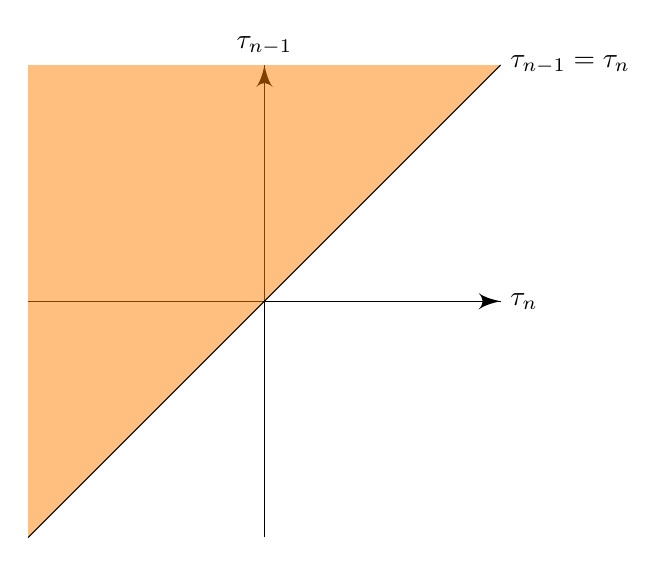
\begin{tikzpicture}
      \draw [->] (-3, 0) -- (3, 0) node [right] {$\tau_n$};
      \draw [->] (0, -3) -- (0, 3) node [above] {$\tau_{n - 1}$};

      \fill [opacity=0.5, morange] (-3, -3) -- (3, 3) -- (-3, 3) -- cycle;
      \draw (-3, -3) -- (3, 3) node [right] {$\tau_{n - 1} = \tau_n$};
    \end{tikzpicture}
  \end{center}
  So we find that
  \[
    S_T = \sum_n (+i)^n \int_{-\infty}^\infty \d \tau_1 \int_{-\infty}^{\tau_1} \d \tau_2 \cdots \int_{-\infty}^{\tau_{n - 1}} \d \tau_n \; V(\tau_n) V(\tau_{n - 1}) \cdots V(\tau_1).
  \]
  We can then see that this is equal to $S^\dagger$.

  What does this tell us? Consider states $\bket{\eta}$ and $\bket{\xi}$ with
  \begin{align*}
    \bket{\eta_T} &= \hat{T} \bket{\eta}\\
    \bket{\xi_T} &= \hat{T} \bket{\xi}
  \end{align*}
  The Dirac bra-ket notation isn't very useful when we have anti-linear operators. So we will write inner products explicitly. We have
  \begin{align*}
    (\eta_T, S\xi_T) &= (\hat{T} \eta, S\hat{T} \xi) \\
    &= (\hat{T} \eta, S_T^\dagger \hat{T} \xi) \\
    &= (\hat{T} \eta, \hat{T} S^\dagger, \xi) \\
    &= (\eta, S^\dagger \xi)^* \\
    &= (\xi, S\eta)
  \end{align*}
  where we used the fact that $\hat{T}$ is anti-unitary. So the conclusion is
  \[
    \brak{\eta_T} S\bket{\xi_T} = \brak{\xi}S\bket{\eta}.
  \]
  So if
  \[
    \hat{T} \mathcal{L}_I(x) \hat{T}^{-1} = \mathcal{L}_I(x_T),
  \]
  then the $S$-matrix elements are equal for time-reversed processes, where the initial and final states are swapped.
\end{eg}

\subsection{CPT theorem}
\begin{thm}[CPT theorem]\index{CPT theorem}
  Any Lorentz invariant Lagrangian with a Hermitian Hamiltonian should be invariant under the product of P, C and T.
\end{thm}
We will not prove this. For details, one can read Streater and Wightman, \emph{PCT, spin and statistics and all that} (1989).

All observations we make suggest that CPT is respected in nature. This means a particle propagating forwards in time cannot be distinguished from the antiparticle propagating backwards in time.

\subsection{Baryogenesis}
In the universe, we observe that there is much more matter than anti-matter. \emph{Baryogenesis}\index{baryogenesis} is the generation of this asymmetry in the universe. Sakarhov came up with three conditions that are necessary for this to happen.
\begin{enumerate}
  \item Baryon number violation (or leptogenesis, i.e.\ lepton number asymmetry), i.e.\ some process $X \to Y + B$ that generates an excess baryon.
  \item Non-equilibrium. Otherwise, the rate of $Y + B \to X$ is the same as the rate of $X \to Y + B$.
  \item C and CP violation. We need C violation, or else the rate of $X \to Y + B$ and the rate of $\bar{X} \to \bar{Y} + \bar{B}$ would be the same, and the effects cancel out each other.

    We similarly need CP violation, or else the rate of $X \to nq_L$ and the rate of $X \to n q_R$, where $q_{L, R}$ are left and right handed quarks, is equal to the rate of $\bar{x} \to n \bar{q}_L$ and $\bar{x} \to n\bar{q}_R$, and this will wash out our excess.
\end{enumerate}

\section{Spontaneous symmetry breaking}
In this chapter, we are going to look at spontaneous symmetry breaking. The general setting is as follows --- our Lagrangian $\mathcal{L}$ enjoys some symmetry. However, the potential has \emph{multiple} minima. Usually, in perturbation theory, we imagine we are sitting near an equilibrium point of the system (the ``vacuum''), and then look at what happens to small perturbations near the equilibrium.

When there are multiple minima, we have to arbitrarily pick a minimum to be our vacuum, and then do perturbation around it. In many cases, this choice of minimum is \emph{not} invariant under our symmetries. Thus, even though the theory itself is symmetric, the symmetry is lost once we pick a vacuum. It turns out interesting things happen when this happens.

\subsection{Discrete symmetry}
We begin with a toy example, namely that of a discrete symmetry. Consider a real scalar field $\phi(x)$ with a symmetric potential $V(\phi)$, so that
\[
  V(-\phi) = V(\phi).
\]
This gives a discrete $\Z/2\Z$ symmetry $\phi \leftrightarrow -\phi$.

We will consider the case of a $\phi^4$ theory, with Lagrangian
\[
  \mathcal{L} = \frac{1}{2} \partial_\mu \phi \partial^\mu \phi - \left(\frac{1}{2} m^2 \phi^2 - \frac{\lambda}{4!} \phi^4\right)
\]
for some $\lambda$.

We want the potential to $\to \infty$ as $\phi \to \infty$, so we necessarily require $\lambda > 0$. However, since the $\phi^4$ term dominates for large $\phi$, we are now free to pick the sign of $m^2$, and still get a sensible theory.

Usually, this theory has $m^2 > 0$, and thus $V(\phi)$ has a minimum at $\phi = 0$:
\begin{center}
  \begin{tikzpicture}
    \draw [->](-3, 0) -- (3, 0) node [right] {$\phi$};
    \draw [->] (0, -1.2) -- (0, 3) node [above] {$S(\phi)$};

    \draw [mblue, thick, domain=-1.414:1.414, samples=50] plot [smooth] (\x, {4 * ((\x/2)^4 + (\x/2)^2)});
  \end{tikzpicture}
\end{center}
However, we could imagine a scenario where $m^2 < 0$, where we have ``imaginary mass''. In this case, the potential looks like
\begin{center}
  \begin{tikzpicture}
    \draw [->](-3, 0) -- (3, 0) node [right] {$\phi$};
    \draw [->] (0, -1.2) -- (0, 3) node [above] {$V(\phi)$};

    \draw [mblue, thick, domain=-2.4:2.4, samples=50] plot [smooth] (\x, {4 * ((\x/2)^4 - (\x/2)^2)});

    \draw [dashed] (1.414, 0) node [above] {$v$} -- (1.414, -1);
  \end{tikzpicture}
\end{center}
To understand this potential better, we complete the square, and write it as
\[
  V(\phi) = \frac{\lambda}{4} (\phi^2 - v^2)^2 + \text{constant},
\]
where
\[
  v = \sqrt{-\frac{m^2}{\lambda}}.
\]
We see that now $\phi = 0$ becomes a local maximum, and there are two (global) minima at $\phi = \pm v$. In particular, $\phi$ has acquired a non-zero \term{vacuum expectation value} (\term{VEV}).

We shall wlog consider small excitations around $\phi = v$. Let's write
\[
  \phi(x) = v + cf(x).
\]
Then we can write the Lagrangian as
\[
  \mathcal{L} = \frac{1}{2} \partial_\mu f \partial^\mu f - \lambda \left(v^2 f^2 + + vf^3 + \frac{1}{4} f^4\right),
\]
plus some constants. Therefore $f$ is a scalar field with mass
\[
  m_f^2 = 2v^2 \lambda.
\]
This $\mathcal{L}$ is \emph{not} invariant under $f \to -f$. The symmetry of the original Lagrangian has been broken by the VEV of $\phi$.

\subsection{Continuous symmetry}
We can consider a slight generalization of the above scenario. Consider an $N$-component real scalar field $\phi = (\phi_1, \phi_2, \cdots, \phi_N)^T$, with Lagrangian
\[
  \mathcal{L} = \frac{1}{2} (\partial^\mu \phi) \cdot (\partial_\mu \phi) - V(\phi),
\]
where
\[
  V(\phi) = \frac{1}{2} m^2 \phi^2 + \frac{\lambda}{4} \phi^4.
\]
As before, we will require that $\lambda > 0$.

This is a theory that is invariant under global $\Or(N)$ transforms of $\phi$. Again, if $m^2 > 0$, then $\phi = 0$ is a global minimum, and we do not have spontaneous symmetry breaking. Thus, we consider the case $m^2 < 0$.

In this case, we can write
\[
  V(\phi) = \frac{\lambda}{4} (\phi^2 - v^2)^2 + \text{constant},
\]
where
\[
  v = -\frac{m^2}{\lambda} > 0.
\]
So \emph{any} $\phi$ with $\phi^2 = v^2$ gives a global minimum of the system, and so we have a continuum of vacua. We call this a \term{Sombrero potential} (or \term{wine bottle potential}).
\begin{center}
  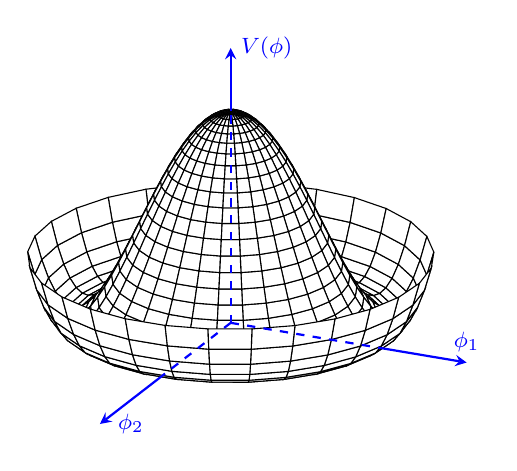
\begin{tikzpicture}
    \begin{axis}[
        hide axis,
        samples=30,
        domain=0:360,
        y domain=0:1.25,clip=false
      ]
      \addplot3 [surf, shader=flat, draw=black, fill=white, z buffer=sort] ({sin(x)*y}, {cos(x)*y}, {(y^2-1)^2});
      \draw[blue,thick,dashed] (axis cs:0,0,0) -- (axis cs:1,0,0);
      \draw[blue,thick,-stealth] (axis cs:1,0,0) -- (axis cs:1.6,0,0) node[above,font=\footnotesize]{$\phi_1$};
      \draw[blue,thick,dashed] (axis cs:0,0,0) -- (axis cs:0,-1,0);
      \draw[blue,thick,-stealth] (axis cs:0,-1,0) -- (axis cs:0,-1.9,0) node[right=1mm,font=\footnotesize]{$\phi_2$};
      \draw[blue,thick,dashed] (axis cs:0,0,0) -- (axis cs:0,0,1);
      \draw[blue,thick,-stealth] (axis cs:0,0,1) -- (axis cs:0,0,1.3) node[right,font=\footnotesize]{$V(\phi)$};
    \end{axis}
  \end{tikzpicture}
\end{center}
Without loss of generality, we may choose the vacuum to be
\[
  \phi_0 = (0, 0, \cdots, 0, v)^T.
\]
We can then consider steady small fluctuations about this:
\[
  \phi(x) = (\pi_1(x), \pi_2(x), \cdots, \pi_{N-1}(x), v + \sigma(x))^T.
\]
We now have a $\pi$ field with $N - 1$ components, plus a $1$-component $\sigma$ field.

We rewrite the Lagrangian in terms of the $\pi$ and $\sigma$ fields as
\[
  \mathcal{L} = \frac{1}{2}(\partial^\mu \pi) \cdot (\partial_\mu \pi) + \frac{1}{2}(\partial^\mu \sigma) \cdot (\partial_\mu \sigma) - V(\pi, \sigma),
\]
where
\[
  V(\pi, \sigma) = \frac{1}{2} m_\sigma^2 \sigma^s + \lambda v(\sigma^2 + \pi^2) \sigma + \frac{\lambda}{4}(\sigma^2 + \pi^2)^2.
\]
Again, we have dropped a constant term.

In this Lagrangian, we see that the $\sigma$ field has mass
\[
  m_\sigma = \sqrt{2\lambda v^2},
\]
but the $\pi$ fields are massless. We can understand this as follows --- the $\sigma$ field corresponds to the radial direction in the potential, and this is locally quadratic, and hence has a mass term. However, the $\pi$ fields correspond to the excitations in the azimuthal directions, which are flat.

\subsection{General case}
What we just saw is a completely general phenomenon. Suppose we have an $N$-dimensional field $\phi = (\phi_1, \cdots, \phi_N)$, and suppose our theory has a Lie group of symmetries $G$. We will assume that the action of $G$ preserves the potential and kinetic terms individually, and not just the Lagrangian as a whole, so that $G$ will send a vacuum to another vacuum.

Suppose there is more than one choice of vacuum. We write
\[
  \Phi_0 = \{\phi_0: V(\phi_0) = V_{\mathrm{min}}\}
\]
for the set of all vacua. Now we pick a favorite vacuum $\phi_0 \in \Phi_0$, and we want to look at the elements of $G$ that fix this vacuum. We write
\[
  H = \stab(\phi_0) = \{h \in G: h \phi_0 = \phi_0\}.
\]
This is the \term{invariant subgroup}, or \term{stabilizer subgroup} of $\phi_0$, and is the symmetry we are left with after the spontaneous symmetry breaking.

We will make some further simplifying assumptions. We will suppose $G$ acts \emph{transitively} on $\Phi_0$, i.e.\ given any two vacua $\phi_0, \phi_0'$, we can find some $g \in G$ such that
\[
  \phi_0' = g \phi_0.
\]
This ensures that any two vacua are ``the same'', so which $\phi_0$ we pick doesn't really matter. Indeed, given two such vacua and $g$ relating them, it is a straightforward computation to check that
\[
  \stab(\phi_0') = g \stab(\phi_0) g^{-1}.
\]
So any two choices of vacuum will result in conjugate, and in particular isomorphic, subgroups $H$.

It is a curious, and also unimportant, observation that given a choice of vacuum $\phi_0$, we have a canonical bijection
\[
  \begin{tikzcd}[cdmap]
    G/H \ar[r, "\sim"] & \Phi_0\\
    g \ar[r, maps to] & g \phi_0
  \end{tikzcd}.
\]
So we can identify $G/H$ and $\Phi_0$. This is known as the orbit-stabilizer theorem.

We now try to understand what happens when we try to do perturbation theory around our choice of vacuum. At $\phi = \phi_0 + \delta \phi$, we can as usual write
\[
  V(\phi_0 + \delta \phi) - V(\phi_0) = \frac{1}{2} \delta \phi_r \frac{\partial^2 V}{\partial \phi_r \partial \phi_s} \delta \phi_s + O(\delta \phi^3).
\]
This quadratic $\partial^2 V$ term is now acting as a mass. We call it the \term{mass matrix}
\[
  M_{rs}^2 = \frac{\partial^2 V}{\partial \phi_r \partial \phi_s}.
\]
Note that we are being sloppy with where our indices go, because $(M^2)^{rs}$ is ugly. It doesn't really matter much, since $\phi$ takes values in $\R^N$ (or $\C^n$), which is a Euclidean space.

In our previous example, we saw that there were certain modes that went massless. We now want to see if the same happens. To do so, we pick a basis $\{\tilde{t}^a\}$ of $\mathfrak{h}$ (the Lie algebra of $H$), and then extend it to a basis $\{t^a, \theta^a\}$ of $\mathfrak{g}$.

We consider a variation
\[
  \delta \phi = \varepsilon \theta^a \phi_0
\]
around $\phi_0$.

Note that when we write $\theta^a \phi_0$, we mean the resulting infinitesimal change of $\phi_0$ when $\theta^a$ acts on field. For a general Lie algebra element, this may be zero. However, we know that $\theta^a$ does not belong to $\mathfrak{h}$, so it does not fix $\phi_0$. Thus (assuming sensible non-degeneracy conditions) this implies that $\theta^a \phi_0$ is non-zero.

At this point, the uncareful reader might be tempted to say that since $G$ is a symmetry of $V$, we must have $V(\phi_0 + \delta \phi) = V(\phi_0)$, and thus
\[
  (\theta^a \phi)_r M_{rs}^2 (\theta^a \phi)_s = 0,
\]
and so we have found zero eigenvectors of $M_{rs}$. But this is wrong. For example, if we take
\[
  M =
  \begin{pmatrix}
    1 & 0\\
    0 & -1
  \end{pmatrix},\quad
  \theta^a \phi =
  \begin{pmatrix}
    1\\1
  \end{pmatrix},
\]
then our previous equation holds, but $\theta^a \phi$ is \emph{not} a zero eigenvector. We need to be a bit more careful.

Instead, we note that by definition of $G$-invariance, for any field value $\phi$ and a corresponding variation
\[
  \phi \mapsto \phi + \varepsilon \theta^a \phi,
\]
we must have
\[
  V(\phi + \delta \phi) = V(\phi),
\]
since this is what it means for $G$ to be a symmetry.

Expanding to first order, this says
\[
  V(\phi + \delta \phi) - V(\phi) = \varepsilon (\theta^a \phi)_r \frac{\partial V}{\partial \phi_r} = 0.
\]
Now the trick is to take a further derivative of this. We obtain
\[
  0 = \frac{\partial}{\partial \phi_s} \left((\theta^a \phi)_r \frac{\partial V}{\partial \phi_r}\right) = \left(\frac{\partial}{\partial \phi_s} (\theta^a \phi)_r\right) \frac{\partial V}{\partial \phi_r} + (\theta^a \phi)_r M_{rs}^2.
\]
Now at a vacuum $\phi = \phi_0$, the first term vanishes. So we must have
\[
  (\theta^a \phi_0)_r M_{rs}^2 = 0.
\]
By assumption, $\theta^a \phi_0 \not= 0$. So we have found a zero vector of $M_{rs}$. Recall that we had $\dim G - \dim H$ of these $\theta^a$ in total. So we have found $\dim G - \dim H$ zero eigenvectors in total.

We can do a small sanity check. What if we replaced $\theta^a$ with $t^a$? The same derivations would still follow through, and we deduce that
\[
  (t^a \phi_0)_r M_{rs}^2 = 0.
\]
But since $t^a$ is an \emph{unbroken symmetry}, we actually just have $t^a \phi_0 = 0$, and this really doesn't say anything interesting.

What about the other eigenvalues? They could be zero for some other reason, and there is no reason to believe one way or the other. However, generally, in the scenarios we meet, they are usually massive. So after spontaneous symmetry breaking, we end up with $\dim G - \dim H$ massless modes, and $N - (\dim G - \dim H)$ massive ones.

This is \term{Goldstone's theorem} in the classical case.
\begin{eg}
  In our previous $O(N)$ model, we had $G = O(N)$, and $H = O(N - 1)$. These have dimensions
  \[
    \dim G = \frac{N(N - 1)}{2},\quad \dim H = \frac{(N - 1)(N - 2)}{2}.
  \]
  Then we have
  \[
    \Phi_0 \cong S^{N - 1},
  \]
  the $(N - 1)$-dimensional sphere. So we expect to have
  \[
    \frac{N - 1}{2} (N - (N - 2)) = N - 1
  \]
  massless modes, which are the $\pi$ fields we found. We also found $N - (N - 1) = 1$ massive mode, namely the $\sigma$ field.
\end{eg}

\begin{eg}
  In the first discrete case, we had $G = \Z/2\Z$ and $H = \{e\}$. These are (rather degenerate) $0$-dimensional Lie groups. So we expect $0 - 0 = 0$ massless modes, and $1 - 0 = 1$ massive modes, which is what we found.
\end{eg}
\subsection{Goldstone's theorem}
We now consider the quantum version of Goldstone's theorem. We hope to get something similar.

Again, suppose our Lagrangian has a symmetry group $G$, which is spontaneously broken into $H \leq G$ after picking a preferred vacuum $\bket{0}$. Again, we take a Lie algebra basis $\{t_a, \theta_a\}$ of $\mathfrak{g}$, where $\{t_a\}$ is a basis for $\mathfrak{h}$. Note that we will assume that $a$ runs from $1, \cdots, \dim G$, and we use the first $\dim H$ labels to refer to the $t_a$, and the remaining to label the $\theta_a$, so that the actual basis is
\[
  \{t_1, t_2, \cdots, t_{\dim H}, \theta_{\dim H + 1}, \cdots, \theta_{\dim G}\}.
\]
For aesthetic reasons, this time we put the indices on the generators below.

Now recall, say from AQFT, that these symmetries of the Lagrangian give rise to conserved currents $j_a^\mu(x)$. These in turn give us conserved charges
\[
  Q_a = \int \d^3 x\; j^0_a (x).
\]
Moreover, under the action of the $t^a$ and $\theta^a$, the corresponding change in $\phi$ is given by
\[
  \delta \phi = -[Q^a, \phi].
\]
The fact that the $\theta^a$ break the symmetry of $\bket{0}$ tells us that, for $a > \dim H$,
\[
  \brak{0}[Q^a, \phi(0)] \bket{0} \not= 0.
\]
Note that the choice of evaluating $\phi$ at $0$ is completely arbitrary, but we have to pick somewhere, and $0$ is easy to write. Writing out the definition of $Q_a$, we know that
\[
  \int \d^3 x\; \brak{0} [j_a^0(x), \phi(0)] \bket{0} \not= 0.
\]
More generally, since the label $^0$ is arbitrary by Lorentz invariance, we are really looking at the relation
\[
  \brak{0} [j_a^\mu (x), \phi(0)] \bket{0} \not= 0,
\]
and writing it in this more Lorentz covariant way makes it easier to work with. The goal is to deduce the existence of massless states from this non-vanishing.

For convenience, we will write this expression as
\[
  X_a^\mu = \brak{0} [j_a^\mu (x), \phi(0)] \bket{0}.
\]
We treat the two terms in the commutator separately. The first term is
\[
  \brak{0} j_a^\mu (x) \phi(0) \bket{0} = \sum_n \brak{0}j_a^\mu (x) \bket{n} \brak{n}\phi(0) \bket{0}.\tag{$*$}
\]
We write $p_n$ for the momentum of $\bket{n}$. We now note the operator equation
\[
  j_a^\mu (x) = e^{i\hat{p} \cdot x} j_a^\mu (0) e^{-i\hat{p} \cdot x}.
\]
So we know
\[
  \brak{0}j_a^\mu(x) \bket{n} = \brak{0} j_a^\mu(0) \bket{n} e^{-ip_n \cdot x}.
\]
We can use this to do some Fourier transform magic. By direct verification, we can see that $(*)$ is equivalent to
\[
  i \int \frac{\d^4 k}{(2\pi)^3} \rho_a^\mu(k) e^{-ik\cdot x},
\]
where
\[
  i \rho_a^\mu (k) = (2\pi)^3 \sum_n \delta^4(k - p_n)\brak{0}j_a^\mu(0) \bket{n} \brak{n}\phi(0)\bket{0}.
\]
Similarly, we define
\[
  i \tilde{\rho}_a^\mu (k) = (2\pi)^3 \sum_n \delta^4(k - p_n) \brak{0} \phi(0) \bket{n} \brak{n} j_a^\mu (0) \bket{0}.
\]
Then we can write
\[
  X_a^\mu = i \int \frac{\d^4 k}{(2\pi)^3}\left(\rho_a^\mu (k) e^{-ik\cdot x} - \tilde{\rho}_a^\mu(k) e^{+ik\cdot x}\right).
\]
This is called the \term{K\"allen-Lehmann spectral representation}.

We now claim that $\rho_a^\mu(k)$ and $\tilde{\rho}_a^\mu(k)$ can be written in a particularly nice form. This involves a few observations (when I say $\rho_a^\mu$, I actually mean $\rho_a^\mu$ and $\tilde{\rho}_a^\mu$):
\begin{itemize}
  \item $\rho_a^\mu$ depends Lorentz covariantly in $k$. So it ``must'' be a scalar multiple of $k^\mu$.
  \item $\rho_a^\mu(k)$ must vanish when $k^0 > 0$, since $k^0 \leq 0$ is non-physical. % why?
  \item By Lorentz invariance, the magnitude of $\rho_a^\mu(k)$ can depend only on the length (squared) $k^2$ of $k$.
\end{itemize}
Under these assumptions, we can write can write $\rho_a^\mu$ and $\tilde{\rho}_a^\mu$ as
\begin{align*}
  \rho_a^\mu (k) &= k^\mu \Theta(k^0) \rho_a (k^2),\\
  \tilde{\rho}_a^\mu (k) &= k^\mu \Theta(k^0) \tilde{\rho}_a(k^2),
\end{align*}
where $\Theta$ is the \term{Heaviside theta function}
\[
  \Theta(x) =
  \begin{cases}
    1 & x > 0\\
    0 & x \leq 0
  \end{cases}.
\]
So we can write
\[
  X_a^\mu = i \int \frac{\d^4 k}{(2\pi)^3}\;k^\mu \Theta(k^0) (\rho_a(k^2)e^{-ik\cdot x} - \tilde{\rho}_a(k^2) e^{+ik\cdot x}).
\]
We now use the (nasty?) trick of hiding the $k^\mu$ by replacing it with a derivative:
\[
  X_a^\mu = - \partial^\mu \int \frac{\d^4 k}{(2\pi)^3} \Theta(k^0)\left(\rho_a(k^2) e^{-ik\cdot x} + \tilde{\rho}_a(k^2) e^{ik\cdot x}\right).
\]
Now we might find the expression inside the integral a bit familiar. Recall that the propagator is given by
\[
  D(x, \sigma) = \brak{0} \phi(x) \phi(0) \bket{0} = \int \frac{\d^4 k}{(2\pi)^3}\; \Theta(k^0) \delta(k^2 - \sigma) e^{-ik\cdot x}.
\]
where $\sigma$ is the square of the mass of the field. Using the really silly fact that
\[
  \rho_a(k^2) = \int \d \sigma\; \rho_a(\sigma) \delta(k^2 - \sigma),
\]
we find that
\[
  X_a^\mu = -\partial^\mu \int \d \sigma\; (\rho_a(\sigma) D(x, \sigma) + \tilde{\rho}_a (\sigma) D(-x, \sigma)).
\]
Now we have to recall more properties of $D$. For spacelike $x$, we have $D(x, \sigma) = D(-x, \sigma)$. Therefore, requiring $X_a^\mu$ to vanish for spacelike $x$ by causality, we see that we must have
\[
  \rho_a(\sigma) = - \tilde{\rho}_a(\sigma).
\]
Therefore we can write
\[
  X_a^\mu = -\partial^\mu \int \d \sigma\; \rho^a(\sigma) i\Delta(x, \sigma),\tag{$\dagger$}
\]
where
\[
  i \Delta(x, \sigma) = D(x, \sigma) - D(-x, \sigma) = \int \frac{\d^4 k}{(2\pi)^3} \delta(k^2 - \sigma) \varepsilon(k^0) e^{-ik\cdot x},
\]
and
\[
  \varepsilon(k^0) =
  \begin{cases}
    +1 & k^0 > 0\\
    -1 & k^0 < 0
  \end{cases}.
\]
This $\Delta$ is again a different sort of propagator.

We now use current conservation, which tells us
\[
  \partial_\mu j^\mu_a = 0.
\]
So we must have
\[
  \partial_\mu X_a^\mu =- \partial^2 \int \d \sigma\; \rho_a(\sigma) i \Delta(x, \sigma) = 0.
\]
On the other hand, by inspection, we see that $\Delta$ satisfies the Klein-Gordon equation
\[
  (\partial^2 + \sigma) \Delta = 0.
\]
So in $(\dagger)$, we can replace $-\partial^2 \Delta$ with $\sigma \Delta$. So we find that
\[
  \partial_\mu X_a^\mu = \int \d \sigma\; \sigma \rho^a (\sigma) i \Delta(x, \sigma) = 0.
\]
This is true for all $x$. In particular, it is true for timelike $x$ where $\Delta$ is non-zero. So we must have
\[
  \sigma \rho_a(\sigma) = 0.
\]
But we also know that $\rho_a(\sigma)$ cannot be identically zero, because $X_a^\mu$ is not. So the only possible explanation is that
\[
  \rho_a(\sigma) = N_a \delta(\sigma),
\]
where $N_a$ is a dimensionful non-zero constant.

Now we retrieve our definitions of $\rho_a$. Recall that they are defined by
\begin{align*}
  i \rho_a^\mu (k) &= (2\pi)^3 \sum_n \delta^4(k - p_n)\brak{0}j_a^\mu(0) \bket{n} \brak{n}\phi(0)\bket{0}\\
  \rho_a^\mu (k) &= k^\mu \Theta(k^0) \rho_a (k^2).
\end{align*}
So the fact that $\rho_a(\sigma) = N_a \delta(\sigma)$ implies that there must be some states, which we shall call $\bket{B(p)}$, of momentum $p$, such that $p^2 = 0$, and
\begin{align*}
  \brak{0}j_a^\mu(0)\bket{B(p)} &\not= 0\\
  \brak{B(p)} \phi(0) \bket{0} &\not= 0.
\end{align*}
The condition that $p^2 = 0$ tell us these particles are massless, which are those massless modes we were looking for! These are the \term{Goldstone bosons}.

We can write the values of the above as
\begin{align*}
  \brak{0} j_a^\mu (0)\bket{B(p)} &= i F_a^B p^\mu\\
  \brak{B(p)} \phi(0)\bket{0} &= Z^B,
\end{align*}
whose form we deduced by Lorentz in/covariance. By dimensional analysis, we know $F_{aB}$ is a dimension $-1$ constant, and $Z_B$ is a dimensionless constant.

From these formulas, we note that since $\phi(0)\bket{0}$ is rotationally invariant, we deduce that $\bket{B(p)}$ also is. So we deduce that these are in fact spin $0$ particles.

Finally, we end with some computations that relate these different numbers we obtained. We will leave the computational details for the reader, and just outline what we should do. Using our formula for $\rho$, we find that
\[
  \brak{0} [j_a^\mu(x), \phi(0)] \bket{0} = - \partial^\mu \int N^a \delta (\sigma) i \Delta(x, \sigma) \;\d \sigma = -iN^a \partial^\mu \Delta(x, 0).
\]
Integrating over space, we find
\[
  \brak{0}[Q_a, \phi(0)]\bket{0} = - iN_a \int \d^3 x\; \partial^0 \Delta(x, 0) = i N_a.
\]
Then we have
\[
  \brak{0} t_a \phi(0)\bket{0} = i \brak{0} [Q_a, \phi(0)]\bket{0} = i \cdot i N_a = -N_a.
\]
So this number $N_a$ sort-of measures how much the symmetry is broken, and we once again see that it is the breaking of symmetry that gives rise to a non-zero $N_a$, hence the massless bosons.

We also recall that we had
\[
  i k^\mu \Theta(k^0) N_a \delta(k^2) = \sum_B \int \frac{\d^3 p}{2|\mathbf{p}|}\; \delta^4(k - p) \brak{0} j_a^\mu(0) \bket{B(p)} \brak{B(p)} \phi(0) \bket{0}.
\]
On the RHS, we can plug in the names we gave for the matrix elements, and on the left, we can write it as an integral
\[
  \int \frac{\d^3 p}{2|\mathbf{p}|} \delta^4 (k - p) i k^\mu N_a = \int \frac{\d^3 p}{2|\mathbf{p}|} \delta^4(k - p) i p^\mu \sum_B F_a^B Z^B.
\]
So we must have
\[
  N^a = \sum_B F_a^B Z^B.
\]
We can repeat this process for each independent symmetry-breaking $\theta^a \in \mathfrak{g} \setminus \mathfrak{h}$, and obtain a Goldstone boson this way. So all together, at least superficially, we find
\[
  n = \dim G - \dim H
\]
many Goldstone bosons.

%The number of broken generators is
%\[
% n = \dim G - \dim H.
%\]
%So we see that there are $n$ of the $\rho^a$ that have non-zero contributions at $\sigma = 0$.
%
%Here $F_{aB}$ is a rank $n$ matrix, and this gives rise to $n$ Goldstone bosons $B$.

It is important to figure out the assumptions we used to derive the result. We mentioned ``Lorentz invariance'' many times in the proof, so we certainly need to assume our theory is Lorentz invariant.
%While it may not seem obvious, the proof actually requires there are more than $2$ spacetime dimensions, and in fact the result does not hold in $2$ or $1$ dimensions.
Another perhaps subtle point is that we also needed states to have a positive definite norm. It turns out in the case of gauge theory, these do not necessarily hold, and we need to work with them separately. % revisit

%Note that we assumed we have a Lorentz invariant theory, and we also assumed there were more than $2$ spacetime dimensions. We don't get spontaneous symmetry breaking in $2$ or $1$ dimensions. We also assumed that states have a positive definite norm. % something about things cancelling.


%We now consider spontaneous symmetry breaking in a fully quantum way. Again, the symmetry group $G$ of the Lagrangian is broken spontaneously to $H \leq G$. In other words, the scalar field gets a non-zero vacuum expectation value
%\[
% \brak{0} \phi(x) \bket{0} = \phi_0 \not= 0.
%\]
%The VEV is invariant under $h \in H$, and so
%\[
% \brak{0} h \phi(x) \bket{0} = \phi_0,
%\]
%but this is not invariant under a general $g \in G \setminus H$. Again suppose we have a basis
%\[
% t^a = \{\tilde{t}^i, \tilde{\theta}^{\tilde{a}}\}
%\]
%of $\mathfrak{g}$, where $\tilde{t}^i$ span $\mathfrak{h} \leq \mathfrak{g}$.
%
%Since $G$ is a symmetry of the Lagrangian, we know there are conserved currents and charges, say $j_a^\mu (x)$ and
%\[
% Q_a = \int \d^3 x\; j^0_a = \int \d^3 x\; \pi(x) t_a \phi,
%\]
%where $\pi$ is the conjugate field. Using the canonical commutation relations, we have
%\[
% \delta \phi(0) = i \alpha^a t^a \phi(0) = - [Q^a, \phi(0)] \alpha^a.
%\]
%Thus these charges induce a representation on the Lie algebra of $\phi$. % ???
%
%To investigate excitations from spontaneous symmetry breaking, consider the VEV of
%\[
% X_a^\mu = \brak{0}[j_a^\mu (x), \phi(0)]\bket{0} = \sum_n \left( \brak{0}j_a^\mu (x) \bket{n} \brak{n}\phi(0) \bket{0} - \brak{0}\phi(0) \bket{n} \brak{n}j_a^\mu(x) \bket{0}\right).
%\]
%We can then write this as
%\[
% i \int \frac{\d^4 k}{(2\pi)^3}\left(\rho_a^\mu (k) e^{-ik\cdot x} - \tilde{\rho}_a^\mu(k) e^{+ik\cdot x}\right),
%\]
%where
%\begin{align*}
% i \rho_a^\mu (k) &= (2\pi)^3 \sum_n \delta^4(k - p_n)\brak{0}j_a^\mu(0) \bket{n} \brak{n}\phi(0)\bket{0}\\
% i \tilde{\rho}_a^\mu (k) &= (2\pi)^3 \sum_n \delta^4(k - p_n) \brak{0} \phi(0) \bket{n} \brak{n} j_a^\mu (0) \bket{0}
%\end{align*}
%Note that we had $j_a^\mu(0)$ because the $e^{-ik\cdot x}$ factors generated the translations. Here $p_n$ is the $4$-momentum of $n$. % ???
%This is called the \term{K\"allen-Lehmann spectral representation}.
%
%From the Lorentz covariance of $\rho_a^\mu$ and $\tilde{\rho}_a^\mu$, they must be proportional to $k^\mu$, as that is the only $4$-vector we have that they can be proportional to. % huh?
%
%Physical states have $k^0 > 0$. Then we can write
%\[
% \rho_a^\mu (k) = k^\mu \Theta(k^0) \rho_a (k^2), % This is k squared.
%\]
%where $\Theta$ is the Heaviside function. Similarly, we have
%\[
% \tilde{\rho}_a^\mu (k) = k^\mu \Theta(k^0) \tilde{\rho}_a(k^2).
%\]
%Then we have
%\[
% X_a^\mu = - \partial^\mu \int \frac{\d^4 k}{(2\pi)^3} \Theta(k^0)\left(\rho_a(k^2) e^{-ik\cdot x} + \tilde{\rho}_a(k^2) e^{ik\cdot x}\right).
%\]
%We can try to relate this to the propagator,
%\[
% D(z - y, \sigma) = \brak{0} \phi(x) \phi(y) \bket{0}, % should be phi(z)
%\]
%where $\sigma$ is the square of the mass of the field. We can write this as
%\[
% D(z - y, \sigma) = \int \frac{\d^4 p}{(2\pi)^3} \Theta(p^0) \delta(p^4 - \sigma) e^{-ip\cdot (z - y)}. % what is p^4?
%\]
%Then we can write
%\[
% X_a^\mu = -\partial_\mu \int \d \sigma (\rho_a(\sigma) D(x, \sigma) + \tilde{\rho}_a (\sigma) D(-x, \sigma)).
%\]
%Here we used the fact that
%\[
% \rho(k^2) = \int \d \sigma\; \rho(\sigma) \delta(k^2 - \sigma).
%\]
%Now for spacelike $x$, we have $D(x, \sigma) = D(-x, \sigma)$. Therefore, requiring $X_a^\mu$ to vanish for spacelike $x$ by causality, we see that
%\[
% \rho_a(\sigma) = - \tilde{\rho}_a(\sigma).
%\]
%Therefore we can write
%\[
% X_a^\mu = -\partial^\mu \int \d \sigma\; \rho^a(\sigma) i\Delta(x, \sigma),\tag{$\dagger$}
%\]
%where
%\[
% i \Delta(x, \sigma) = D(x, \sigma) - D(-x, \sigma) = \int \frac{\d^4 k}{(2\pi)^3} \delta(k^2 - \sigma) \varepsilon(k^0) e^{-ik\cdot x},
%\]
%where
%\[
% \varepsilon(k^0) =
% \begin{cases}
% +1 & k^0 > 0\\
% -1 & k^0 < 0
% \end{cases}.
%\]
%We can think of this as some different sort of propagator. For spacelike $x$, this vanishes.
%
%We now use current conservation, so
%\[
% \partial_\mu j^\mu_a = 0.
%\]
%So we find
%\[
% \partial_\mu X_a^\mu =- \partial^2 \int \d \sigma\; \rho_a(\sigma) i \Delta(x, \sigma) = 0.
%\]
%Also, the Klein-Gordon equation gives
%\[
% (\partial^2 + \sigma) \Delta = 0.
%\]
%So we can replace $-\partial^s \Delta$ with $\sigma \Delta$. So
%\[
% \partial_\mu X_a^\mu = \int \d \sigma\; \sigma \rho^a (\sigma) i \Delta(x, \sigma) = 0.
%\]
%This is true for all $x$. In particular, it is true for timelike $x$ where $\Delta$ is non-zero. So we need
%\[
% \sigma \rho(\sigma) = 0.
%\]
%There are two possibilities:
%\begin{enumerate}
% \item $\rho(\sigma) = 0$. This means
% \[
% \brak{0} [j_a^\mu(x), \phi(0)] \bket{0} = 0.
% \]
% So $t^a$ is an unbroken symmetry, and
% \[
% \brak{0} t^a \phi\bket{0} = 0.
% \]
% \item $\rho^a(\sigma) = N^a \delta(\sigma)$, where $N^a$ is a dimensionful non-zero constant.
%\end{enumerate}
%The first case is boring, so we want to figure out what the consequences of (ii) are. Plugging this into $(\dagger)$, we get
%\[
% \brak{0} [j_a^\mu(x), \phi(0)] \bket{0} = - \partial^\mu \int N^a \delta (\sigma) i \Delta(x, \sigma) \;\d \sigma = -iN^a \partial^\mu \Delta(x, 0).
%\]
%Integrating over time, we find
%\[
% \brak{0}[Q^a, \phi(0)]\bket{0} = - iM^a \int \d^3 x\; \partial^0 \Delta(x, 0) = i N^a.
%\]
%Then we have\[
% \brak{0} t^a \phi_0\bket{0} = i \brak{0} [Q^a, \phi(0)]\bket{0} = i \cdot i N^a = -N^a.
%\]
%Now if $N^a$ and $\phi_0$ are both non-zero, then some states in $\rho_a^\mu$ and $\tilde{\rho}_a^\mu$ have non-zero matrix elements. Label these states by $B(p)$. From Lorentz covariance and dimensional analysis, we have
%\begin{align*}
% \brak{0} j_a^\mu (0)\bket{B(p)} &= i F_{aB} p^\mu\\
% \brak{B(p)} \phi(0)\bket{0} &= Z_B,
%\end{align*}
%where $F_{aB}$ is a dimension $-1$ constant, and $Z_B$ is a dimensionless constnat.
%
%We see that $B(p)$ are spin zero by rotation invariance, and massless (only contribute when $\sigma = p^2 = 0$). We have
%\[
% i \rho_a^\mu (k) = i k^\mu \Theta(k^0) N^a \sigma(k^2) = \sum_B \int \frac{\d^3 p}{2|\mathbf{p}|} \delta^4(k - p) \brak{0} j_a^\mu(0) \bket{B(p)} \brak{B(p)} \phi(0) \bket{0}.
%\]
%We write the LHS as an integral, and plug in the matrix element on the RHS. Then we see that
%\[
% \int \frac{\d^3 p}{2|\mathbf{p}|} \delta^4 (k - p) i k^\mu N^a = \int \frac{\d^3 p}{2|\mathbf{p}|} \delta^4(k - p) i p^\mu \sum_B F_{aB} Z_B.
%\]
%So we have
%\[
% N^a = \sum_B F_{aB} Z_B.
%\]
%The number of broken generators is
%\[
% n = \dim G - \dim H.
%\]
%So we see that there are $n$ of the $\rho^a$ that have non-zero contributions at $\sigma = 0$.
%
%Here $F_{aB}$ is a rank $n$ matrix, and this gives rise to $n$ Goldstone bosons $B$.
%
%Note that we assumed we have a Lorentz invariant theory, and we also assumed there were more than $2$ spacetime dimensions. We don't get spontaneous symmetry breaking in $2$ or $1$ dimensions. We also assumed that states have a positive definite norm. % something about things cancelling.

\subsection{The Higgs mechanism}
Recall that we had a few conditions for our previous theorem to hold. In the case of gauge theories, these typically don't hold. For example, in QED, imposing a Lorentz invariant gauge condition (e.g.\ the Lorentz gauge) gives us negative norm states. On the other hand, if we fix the gauge condition so that we don't have negative norm states, this breaks Lorentz invariance. What happens in this case is known as the \term{Higgs mechanism}.

Let's consider the case of scalar electrodynamics. This involves two fields:
\begin{itemize}
  \item A complex scalar field $\phi(x) \in \C$.
  \item A 4-vector field $A(x) \in \R^{1, 3}$.
\end{itemize}
As usual the components of $A(x)$ are denoted $A_\mu(x)$. From this we define the electromagnetic field tensor
\[
  F_{\mu\nu} = \partial_\mu A_\nu - \partial_\nu A_\mu,
\]
and we have a covariant derivative
\[
  \D_\mu = \partial_\mu + i q A_\mu.
\]
As usual, the Lagrangian is given by
\[
  \mathcal{L} = -\frac{1}{4} F_{\mu\nu} F^{\mu\nu} + (\D_\mu \phi)^* (\D^\mu \phi) - V(|\phi|^2)
\]
for some potential $V$.

A $\U(1)$ gauge transformation is specified by some $\alpha(x) \in \R$. Then the fields transform as
\begin{align*}
  \phi(x) &\mapsto e^{i\alpha(x)} \phi(x)\\
  A_\mu(x) &\mapsto A_\mu(x) - \frac{1}{q} \partial_\mu \alpha(x).
\end{align*}
We will consider a $\phi^4$ theory, so that the potential is
\[
  V(|\phi|^2) = \mu^2 |\phi|^2 + \lambda |\phi|^4.
\]
As usual, we require $\lambda > 0$, and if $\mu^2 > 0$, then this is boring with a unique vacuum at $\phi = 0$. In this case, $A_\mu$ is massless and $\phi$ is massive.

If instead $\mu^2 < 0$, then this is the interesting case. We have a minima at
\[
  |\phi_0|^2 = -\frac{\mu^2}{2\lambda} \equiv \frac{v^2}{2}.
\]
Without loss of generality, we expand around a real $\phi_0$, and write
\[
  \phi(x) = \frac{1}{\sqrt{2}} e^{i \theta(x)/v} (v + \eta(x)),
\]
where $\eta, \theta$ are \emph{real} fields.

Now we notice that $\theta$ isn't a ``genuine'' field (despite being real). Our theory is invariant under gauge transformations. Thus, by picking
\[
  \alpha(x) = - \frac{1}{v} \theta(x),
\]
we can get rid of the $\theta(x)$ term, and be left with
\[
  \phi(x) = \frac{1}{\sqrt{2}}(v + \eta(x)).
\]
This is called the \term{unitary gauge}. Of course, once we have made this choice, we no longer have the gauge freedom, but on the other hand everything else going on becomes much clearer.

%For small fluctuations, we approximate
%\[
% \phi(x) \approx \frac{1}{\sqrt{2}} (v + \eta + i \theta).
%\]
%We will chose $v > 0$. We substitute this into the potential to get
%\[
% V(\phi^* \phi) = \lambda \left(|\phi|^2 - \frac{v^2}{2}\right)^2 = \frac{\lambda}{4} (v^2 + \eta^2 + 2 v \eta - v^2)^2
%\]
%where we as usual dropped a constant. Putting this to the Lagrangian, we get
%\[
% \mathcal{L} = \frac{1}{2} \left(\partial_\mu \eta \partial^\mu \eta + 2 \mu^2 \eta^2\right) + \frac{1}{2} \partial_\mu \theta \partial^\mu \theta - \frac{1}{4} F^{\mu\nu} F_{\mu\nu} + qv A_\mu \partial^\mu \theta + \frac{q^2 v^2}{2} A_\mu A^\mu + \mathcal{L}_{\mathrm{int}},
%\]
%where $\mathcal{L}_{\mathrm{int}}$ involves terms with $\geq 2$ fields.
%
%It appears that that we have a mass for $\eta$ and $A_\mu$, but not $\theta$, and also a strange $A_\mu \partial^\mu \theta$ term.
%
%To see what is going on, we transform to the \term{unitary gauge}.
%\[
% A_\mu \mapsto A_\mu + \frac{1}{qv} \partial_\mu \theta(x),
%\]
%where we have chosen
%\[
% \alpha(x) = - \frac{1}{v} \theta(x).
%\]
%Then the $\phi$ field transforms as
%\[
% \phi \mapsto e^{i\theta/v} \phi = \frac{1}{2} (v + \eta).
%\]
%This corresponds to getting rid of the phase, and so we may assume $\phi$ is real.
In this gauge, the Lagrangian can be written as
\[
  \mathcal{L} = \frac{1}{2}(\partial_\mu \eta \partial^\mu \eta + 2 \mu^2 \eta^2) - \frac{1}{4} F^{\mu\nu}F_{\mu\nu} + \frac{q^2 v^2}{2} A_\mu A^\mu + \mathcal{L}_{\mathrm{int}},
\]
where $\mathcal{L}_{\mathrm{int}}$ is the interaction piece that involves more than two fields.

We can now just read off what is going on in here.
\begin{itemize}
  \item The $\eta$ field is massive with mass
    \[
      m_\mu^2 = - 2 \mu^2 = 2 \lambda v^2 > 0.
    \]
  \item The photon now gains a mass
    \[
      m_A^2 = q^2 v^2.
    \]
  \item What would be the Goldstone boson, namely the $\theta$ field, has been ``eaten'' to become the longitudinal polarization of $A_\mu$ and $A_\mu$ has gained a degree of freedom (or rather, the gauge non-degree-of-freedom became a genuine degree of freedom).
\end{itemize}
One can check that the interaction piece becomes
\[
  \mathcal{L}_{\mathrm{int}} = \frac{q^2}{2} A^\mu A^\mu \eta^2 + q m_A A_\mu A^\mu \eta - \frac{\lambda}{4} \eta^4 - m_\eta \sqrt{\frac{\lambda}{2}} \eta^3.
\]
So we have interactions that look like
\begin{center}
  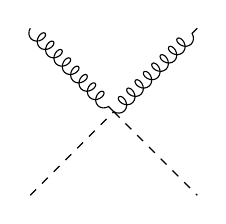
\begin{tikzpicture}
    \begin{feynman}
      \vertex (tl);
      \vertex [below right=of tl] (c);
      \vertex [above right=of c] (tr);
      \vertex [below left=of c] (bl);
      \vertex [below right=of c] (br);

      \diagram*{
        (tl) -- [gluon] (c) -- [gluon] (tr),
        (bl) -- [scalar] (c) -- [scalar] (br)
      };
    \end{feynman}
  \end{tikzpicture}
  \quad
  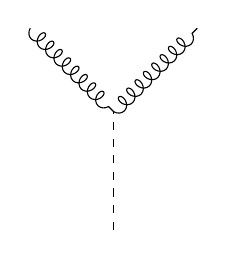
\begin{tikzpicture}
    \begin{feynman}
      \vertex (tl);
      \vertex [below right=of tl] (c);
      \vertex [above right=of c] (tr);
      \vertex [below =of c] (b);

      \diagram*{
        (tl) -- [gluon] (c) -- [gluon] (tr),
        (b) -- [scalar] (c)
      };
    \end{feynman}
  \end{tikzpicture}
  \quad
  \begin{tikzpicture}
    \begin{feynman}
      \vertex (tl);
      \vertex [below right=of tl] (c);
      \vertex [above right=of c] (tr);
      \vertex [below left=of c] (bl);
      \vertex [below right=of c] (br);

      \diagram*{
        (tl) -- [scalar] (c) -- [scalar] (tr),
        (bl) -- [scalar] (c) -- [scalar] (br)
      };
    \end{feynman}
  \end{tikzpicture}
  \quad
  \begin{tikzpicture}
    \begin{feynman}
      \vertex (tl);
      \vertex [below right=of tl] (c);
      \vertex [above right=of c] (tr);
      \vertex [below =of c] (b);

      \diagram*{
        (tl) -- [scalar] (c) -- [scalar] (tr),
        (b) -- [scalar] (c)
      };
    \end{feynman}
  \end{tikzpicture}
\end{center}
This $\eta$ field is the ``Higgs boson'' in our toy theory.

\subsection{Non-abelian gauge theories}
We'll not actually talk about spontaneous symmetry in non-abelian gauge theories. That is the story of the next chapter, where we start studying electroweak theory. Instead, we'll just briefly set up the general framework of non-abelian gauge theory.

In general, we have a gauge group $G$, which is a compact Lie group with Lie algebra $\mathfrak{g}$. We also have a representation of $G$ on $\C^n$, which we will assume is unitary, i.e.\ each element of $G$ is represented by a unitary matrix. Our field $\psi(x) \in \C^n$ takes values in this representation.

A \term{gauge transformation} is specified by giving a $g(x) \in G$ for each point $x$ in the universe, and then the field transforms as
\[
  \psi(x) \mapsto g(x) \psi(x).
\]
Alternatively, we can represent this transformation infinitesimally, by producing some $t(x) \in \mathfrak{g}$, and then the transformation is specified by
\[
  \psi(x) \mapsto \exp(i t(x)) \psi(x).
\]
Associated to our gauge theory is a \term{gauge field} $A_\mu(x) \in \mathfrak{g}$ (i.e.\ we have an element of $\mathfrak{g}$ for each $\mu$ and $x$), which transforms under an infinitesimal transformation $t(x) \in \mathfrak{g}$ as
\[
  A_\mu(x) \mapsto - \partial_\mu t(x) + [t, A_\mu].
\]
The gauge covariant derivative is again give by
\[
  \D_\mu = \partial_\mu + i g A_\mu.
\]
where all fields are, of course, implicitly evaluated at $x$. As before, we can define
\[
  F_{\mu\nu} = \partial_\mu A_\nu - \partial_\nu A_\mu - g [A_\mu, A_\nu] \in \mathfrak{g},
\]
Alternatively, we can write this as
\[
  [\D_\mu, \D_\nu] = ig F_{\mu\nu}.
\]
We will later on work in coordinates. We can pick a basis of $\mathfrak{g}$, say $t^1, \cdots, t^n$. Then we can write an arbitrary element of $\mathfrak{g}$ as $\theta^a(x) t^a$. Then in this basis, we write the components of the gauge field as $A_\mu^a$, and similarly the field strength is denoted $F_{\mu\nu}^a$. We can define the \term{structure constants} \term{$f^{abc}$} by
\[
  [t^a, t^b] = f^{abc}t^c.
\]
Using this notation, the gauge part of the Lagrangian $\mathcal{L}$ is
\[
  \mathcal{L}_g = -\frac{1}{4} F_{\mu\nu}^a F^{a\mu\nu} = - \frac{1}{2} \Tr (F_{\mu\nu} F^{\mu\nu}).
\]
We now move on to look at some actual theories.

\section{Electroweak theory}
We can now start discussing the standard model. In this chapter, we will account for everything in the theory apart from the strong force. In particular, we will talk about the gauge (electroweak) and Higgs part of the theory, as well as the matter content.

The description of the theory will be entirely in the classical world. It is only when we do computations that we quantize the theory and compute $S$-matrices.

\subsection{Electroweak gauge theory}
We start by understanding the gauge and Higgs part of the theory. As mentioned, the gauge group is
\[
  G = \SU(2)_L \times \U(1)_Y.
\]
We will see that this is broken by the Higgs mechanism.

It is convenient to pick a basis for $\su(2)$, which we will denote by
\[
  \tau^a = \frac{\sigma^a}{2}.
\]
Note that these are not genuinely elements of $\su(2)$. We need to multiply these by $i$ to actually get members of $\su(2)$ (thus, they form a complex basis for the complexification of $\su(2)$). As we will later see, these act on fields as $e^{i \tau^a}$ instead of $e^{\tau^a}$. Under this basis, the structure constants are $f^{abc} = \varepsilon^{abc}$.

We start by describing how our gauge group acts on the Higgs field.
\begin{defi}[Higgs field]\index{Higgs field}
  The \emph{Higgs field} $\phi$ is a complex scalar field with two components, $\phi(x) \in \C^2$. The $\SU(2)$ action is given by the fundamental representation on $\C^2$, and the hypercharge is $Y = \frac{1}{2}$.

  Explicitly, an (infinitesimal) gauge transformation can be represented by elements $\alpha^a(x), \beta(x) \in \R$, corresponding to the elements $\alpha^a(x) \tau^a \in \su(2)$ and $\beta(x) \in \uu (1) \cong \R$. Then the Higgs field transform as
  \[
    \phi(x) \mapsto e^{i \alpha^a(x) \tau^a} e^{i \frac{1}{2} \beta(x)} \phi(x),
  \]
  where the $\frac{1}{2}$ factor of $\beta(x)$ comes from the hypercharge being $\frac{1}{2}$.
\end{defi}
Note that when we say $\phi$ is a scalar field, we mean it transforms trivially via Lorentz transformations. It still takes values in the vector space $\C^2$.

The gauge fields corresponding to $\SU(2)$ and $\U(1)$ are denoted $W_\mu^a$ and $B_\mu$, where again $a$ runs through $a = 1, 2, 3$. The covariant derivative associated to these gauge fields is
\[
  \D_\mu = \partial_\mu + i g W_\mu^a \tau^a + \frac{1}{2} i g' B_\mu
\]
for some coupling constants $g$ and $g'$.

The part of the Lagrangian relating the gauge and Higgs field is
\[
  \mathcal{L}_{\mathrm{gauge}, \phi} = -\frac{1}{2} \Tr (F^W_{\mu\nu} F^{W,\mu\nu}) - \frac{1}{4} F_{\mu\nu}^B F^{B, \mu\nu} + (\D_\mu \phi)^\dagger (\D^\mu \phi) - \mu^2 |\phi|^2 - \lambda |\phi|^4,
\]
where the field strengths of $W$ and $B$ respectively are given by
\begin{align*}
  F_{\mu\nu}^{W, a} &= \partial_\mu W_\nu^a - \partial_\nu W_\mu^a - g \varepsilon^{abc} W_\mu^b W_\nu^c\\
  F_{\mu\nu}^B &= \partial_\mu B_\nu - \partial_\nu V_\mu.
\end{align*}
In the case $\mu^2 < 0$, the Higgs field acquires a VEV, and we wlog shall choose the vacuum to be
\[
  \phi_0 = \frac{1}{\sqrt{2}}
  \begin{pmatrix}
    0\\ v
  \end{pmatrix},
\]
where
\[
  \mu^2 = - \lambda v^2 < 0.
\]
As in the case of $\U(1)$ symmetry breaking, the gauge term gives us new things with mass. After spending hours working out the computations, we find that $(\D_\mu \phi)^\dagger (\D^\mu \phi)$ contains mass terms
\[
  \frac{1}{2} \frac{v^2}{4} \left(g^2 (W^1)^2 + g^2 (W^2)^2 + (-gW^3 + g' B)^2\right).
\]
This suggests we define the following new fields:
\begin{align*}
  W_\mu^{\pm} &= \frac{1}{\sqrt{2}} (W_\mu^1 \mp i W_\mu^2)\\
  \begin{pmatrix}
    Z_\mu^0\\
    A_\mu
  \end{pmatrix} &=
  \begin{pmatrix}
    \cos \theta_W & - \sin \theta_W\\
    \sin \theta_W & \cos \theta_W
  \end{pmatrix}
  \begin{pmatrix}
    W_\mu^3\\
    B_\mu
  \end{pmatrix},
\end{align*}
where we pick $\theta_W$ such that
\[
  \cos \theta_W = \frac{g}{\sqrt{g^2 + g'^2}},\quad \sin \theta_W = \frac{g'}{\sqrt{g^2 + g'^2}}.
\]
This $\theta_W$ is called the \term{Weinberg angle}. Then the mass term above becomes
\[
  \frac{1}{2} \left(\frac{v^2g^2}{4} ((W^+)^2 + (W^-)^2) + \frac{v^2(g^2 + g'^2)}{4} Z^2\right).
\]
Thus, our particles have masses
\begin{align*}
  m_W &= \frac{vg}{2}\\
  m_Z &= \frac{v}{2} \sqrt{g^2 + g'^2}\\
  m_\gamma &= 0,
\end{align*}
where $\gamma$ is the $A_\mu$ particle, which is the photon. Thus, our original $\SU(2) \times \U(1)_Y$ breaks down to a $\U(1)_{EM}$ symmetry. In terms of the Weinberg angle,
\[
  m_W = m_Z \cos \theta_W.
\]
Thus, through the Higgs mechanism, we find that the $W^{\pm}$ and $Z$ bosons gained mass, but the photon does not. This agrees with what we find experimentally. In practice, we find that the masses are
\begin{align*}
  m_W &\approx \SI{80}{\giga\electronvolt}\\
  m_Z &\approx \SI{91}{\giga\electronvolt}\\
  m_\gamma &< \SI{e-18}{\giga\electronvolt}.
\end{align*}
Also, the Higgs boson gets mass, as what we saw previously. It is given by
\[
  m_H = \sqrt{-2 \mu^2} = \sqrt{2 \lambda v^2}.
\]
Note that the Higgs mass depends on the constant $\lambda$, which we haven't seen anywhere else so far. So we can't tell $m_H$ from what we know about $W$ and $Z$. Thus, until the Higgs was discovered recently, we didn't know about the mass of the Higgs boson. We now know that
\[
  m_H \approx \SI{125}{\giga\electronvolt}.
\]
Note that we didn't write out all terms in the Lagrangian, but as we did before, we are going to get $W^{\pm}$, $Z$-Higgs and Higgs-Higgs interactions.

One might find it a bit pointless to define the $W^+$ and $W^-$ fields as we did, as the kinetic terms looked just as good with $W^1$ and $W^2$. The advantage of this new definition is that $W_\mu^+$ is now the complex conjugate $W_\mu^-$, so we can instead view the $W$ bosons as given by a single complex scalar field, and when we quantize, $W_\mu^+$ will be the anti-particle of $W_\mu^-$.

\subsection{Coupling to leptons}
We now look at how gauge bosons couple to matter. In general, for a particle with hypercharge $Y$, the covariant derivative is
\[
  \D_\mu = \partial_\mu + i g W_\mu^a \tau^a + i g' Y B_\mu
\]
In terms of the $W^{\pm}$ and $Z$ bosons, we can write this as
\begin{multline*}
  \D_\mu = \partial_\mu + \frac{ig}{\sqrt{2}} (W_\mu^+ \tau^+ + W_\mu^- \tau^-) + \frac{ig Z_\mu}{\cos \theta_W} (\cos^2 \theta_W \tau^3 - \sin^2 \theta_W Y) \\
  + ig \sin \theta_W A_\mu (\tau^3 + Y),
\end{multline*}
where
\[
  \tau^{\pm} = \tau^1 \pm i \tau^2.
\]
By analogy, we interpret the final term $ig \sin \theta_W A_\mu (\tau^3 + Y)$ is the usual coupling with the photon. So we can identify the (magnitude of the) electron charge as
\[
  e = g \sin \theta_W,
\]
while the $\U(1)_{EM}$ charge matrix is
\[
  Q = \U(1)_{EM} = \tau^3 + Y.
\]
If we want to replace all occurrences of the hypercharge $Y$ with $Q$, then we need to note that
\[
  \cos^2 \theta_W \tau^3 - \sin^2 \theta_W Y = \tau^3 - \sin^2 \theta_W Q.
\]
We now introduce the electron field. The electron field is given by a spinor field $e(x)$. We will decompose it as left and right components
\[
  e(x) = e_L(x) + e_R(x).
\]
There is also a neutrino field $\nu_{e_L}(x)$. We will assume that neutrinos are massless, and there are only left-handed neutrinos. We know this is not entirely true, because of neutrinos oscillation, but the mass is very tiny, and this is a very good approximation.

To come up with an actual electroweak theory, we need to specify a representation of $\SU(2) \times \U(1)$. It is convenient to group our particles by handedness:
\[
  R(x) = e_R(x),\quad L(x) =
  \begin{pmatrix}
    \nu_{e_L}(x)\\
    e_L(x)
  \end{pmatrix}.
\]
Here $R(x)$ is a single spinor, while $L(x)$ consists of a \emph{pair}, or ($\SU(2)$) \term{doublet}\index{$\SU(2)$ doublet} of spinors.

We first look at $R(x)$. Experimentally, we find that $W^{\pm}$ only couples to left-handed leptons. So $R(x)$ will have the \emph{trivial representation} of $\SU(2)$. We also know that electrons have charge $Q = -1$. Since $\tau^3$ acts trivially on $R$, we must have
\[
  Q = Y = -1
\]
for the right-handed leptons.

The left-handed particles are more complicated. We will assert that $L$ has the ``fundamental'' representation of $\SU(2)$, by which we mean given a matrix
\[
  g = \begin{pmatrix}
    a & b\\
    -\bar{b} & \bar{a}
  \end{pmatrix}\in \SU(2),
\]
it acts on $L$ as
\[
  g L =
  \begin{pmatrix}
    a & b\\
    - \bar{b} & \bar{a}
  \end{pmatrix}
  \begin{pmatrix}
    \nu_{e_L}\\
    e_L
  \end{pmatrix} =
  \begin{pmatrix}
    a \nu_{e_L} + b e_L\\
    -\bar{b} \nu_{e_L} + \bar{a} e_L
  \end{pmatrix}.
\]
We know the electron has charge $-1$ and the neutrino has charge $0$. So we need
\[
  Q =
  \begin{pmatrix}
    0 & 0 \\
    0 & -1
  \end{pmatrix}.
\]
Since $Q = \tau^3 + Y$, we must have $Y = -\frac{1}{2}$.

Using this notation, the gauge part of the lepton Lagrangian can be written concisely as
\[
  \mathcal{L}_{\mathrm{lepton}}^{EW} = \bar L i \slashed D L + \bar R i \slashed D R.
\]
Note that $\bar{L}$ means we take the transpose of the matrix $L$, viewed as a matrix with two components, and then take the conjugate of each spinor individually, so that
\[
  \bar{L} =
  \begin{pmatrix}
    \bar{\nu}_{e_L}(x) & \bar{e}_L(x)
  \end{pmatrix}.
\]
How about the mass? Recall that it makes sense to deal with left and right-handed fermions separately only if the fermion is massless. A mass term
\[
  m_e (\bar{e}_Le_R + \bar{e}_R e_L)
\]
would be very bad, because our $\SU(2)$ action mixes $e_L$ with $\nu_{e_L}$.

But we do know that the electron has mass. The answer is that the mass is again granted by the spontaneous symmetry breaking of the Higgs boson. Working in unitary gauge, we can write the Higgs boson as
\[
  \phi(x) = \frac{1}{\sqrt{2}}
  \begin{pmatrix}
    0\\
    v + h(x)
  \end{pmatrix},
\]
with $v, h(x) \in \R$.

The lepton-Higgs interactions is given by
\[
  \mathcal{L}_{\mathrm{lept}, \phi} = - \sqrt{2} \lambda_e (\bar L \phi R + \bar R \phi^\dagger L),
\]
where $\lambda_e$ is the \term{Yukawa coupling}. It is helpful to make it more explicit what we mean by this expression. We have
\[
  \bar{L} \phi R =
  \begin{pmatrix}
    \bar{\nu}_{e_L}(x) & \bar{e}_L(x)
  \end{pmatrix}
  \left(
  \frac{1}{\sqrt{2}}
  \begin{pmatrix}
    0\\
    v + h(x)
  \end{pmatrix}
  \right)
  e_R(x) = \frac{1}{\sqrt{2}} (v + h(x)) \bar{e}_L(x) e_R(x).
\]
Similarly, we can write out the second term and obtain
\begin{align*}
  \mathcal{L}_{\mathrm{lept}, \phi} &= - \lambda_e (v + h) (\bar{e}_L e_R + \bar{e}_R e_L)\\
  &= - m_e \bar{e} e - \lambda_e h \bar{e} e,
\end{align*}
where
\[
  m_e = \lambda_e v.
\]
We see that while the interaction term is a priori gauge invariant, once we have spontaneously broken the symmetry, we have magically obtained a mass term $m_e$. The second term in the Lagrangian is the Higgs-fermion coupling. We see that this is proportional to $m_e$. So massive things couple more strongly.

We now return to the fermion-gauge boson interactions. We can write it as
\[
  \mathcal{L}_{\mathrm{lept}}^{EM, \mathrm{int}} = \frac{g}{2\sqrt{2}} (J^\mu W_\mu^+ + J^{\mu\dagger} W_\mu^-) + e J_{EM}^\mu A_\mu + \frac{g}{2 \cos \theta_W} J_n^\mu Z_\mu.
\]
where
\begin{align*}
  J^\mu_{EM} &= - \bar{e} \gamma^\mu e\\
  J^\mu &= \bar{\nu}_{e_L}\gamma^\mu (1 - \gamma^5) e\\
  J^\mu_n &= \frac{1}{2} \left(\bar{\nu}_{e_L} \gamma^\mu (1 - \gamma^5) \nu_{e_L} - \bar{e} \gamma^\mu (1 - \gamma^5 - 4 \sin^2 \theta_w)e\right)
\end{align*}
Note that $J^\mu_{EM}$ has a negative sign because the electron has negative charge. These currents are known as the \term{EM current}, \term{charge weak current} and \term{neutral weak current} respectively.

There is one thing we haven't mentioned so far. We only talked about electrons and neutrinos, but the standard model has three generations of leptons. There are the \term{muon} (\term{$\mu$}) and \term{tau} (\term{$\tau$}), and corresponding left-handed neutrinos. With these in mind, we introduce
\[
  L^1 =
  \begin{pmatrix}
    \nu_{e_L}\\
    e_L
  \end{pmatrix},\quad
  L^2 =
  \begin{pmatrix}
    \nu_{\mu_L}\\
    \mu_L
  \end{pmatrix},\quad
  L^3 =
  \begin{pmatrix}
    \nu_{\tau_L}\\
    \tau_L
  \end{pmatrix}.
\]
\[
  R^1 = e_R,\quad R^2 = \mu_R,\quad R^3 = \tau_R.
\]
These couple and interact in exactly the same way as the electrons, but have heavier mass. It is straightforward to add these into the $\mathcal{L}_{\mathrm{lept}}^{EW, \mathrm{int}}$ term. What is more interesting is the Higgs interaction, which is given by
\[
  \mathcal{L}_{\mathrm{lept}, \phi} = - \sqrt{2} \Big(\lambda^{ij} \bar{L}^i \phi R^j + (\lambda^\dagger)^{ij} \bar{R}^i \phi^\dagger L^j\Big),
\]
where $i$ and $j$ run over the different generations. What's new now is that we have the matrices $\lambda \in M_3(\C)$. These are \emph{not} predicted by the standard model.

This $\lambda$ is just a general matrix, and there is no reason to expect it to be diagonal. However, in some sense, it is always diagonalizable. The key insight is that we contract the two indices $\lambda$ with two \emph{different} kinds of things. It is a general linear algebra fact that for any matrix $\lambda$ at all, we can find some unitary matrices $U$ and $S$ such that
\[
  \lambda = U \Lambda S^\dagger,
\]
where $\Lambda$ is a diagonal matrix with real entries. We can then transform our fields by
\begin{align*}
  L^i &\mapsto U^{ij} L^j\\
  R^i &\mapsto S^{ij} R^j,
\end{align*}
and this diagonalizes $\mathcal{L}_{\mathrm{lept}, \phi}$.

It is also clear that this leaves $\mathcal{L}_{\mathrm{lept}}^{EW}$ invariant, especially if we look at the expression before symmetry breaking. So the mass eigenstates are the same as the ``\term{weak eigenstates}''. This tells us that after diagonalizing, there is no mixing within the different generations.

This is important. It is \emph{not} possible for quarks (or if we have neutrino mass), and mixing \emph{does} occur in these cases.

\subsection{Quarks}
We now move on to study quarks. There are 6 flavours of quarks, coming in three generations:
\begin{center}
  \begin{tabular}{cccc}
    \toprule
    Charge & First generation & Second generation & Third generation\\
    \midrule
    $+\frac{2}{3}$ & Up ($u$) & Charm ($c$) & Top ($t$)\\
    $-\frac{1}{3}$ & Down ($d$) & Strange ($s$) & Bottom ($b$)\\
    \bottomrule
  \end{tabular}
\end{center}
each of which is a spinor.

The right handed fields have trivial $\SU(2)$ representations, and are thus $\SU(2)$ singlets. We write them as
\[
  u_R = \begin{pmatrix} u_R & c_R & t_R\end{pmatrix}
\]
which have $Y = Q = +\frac{2}{3}$, and
\[
  d_R = \begin{pmatrix} d_R & s_R & b_R\end{pmatrix}
\]
which have $Y = Q = -\frac{1}{3}$.

The left-handed fields are in $\SU(2)$ doublets
\[
  Q_L^i =
  \begin{pmatrix}
    u_L^i\\
    d_L^i
  \end{pmatrix} =
  \begin{pmatrix}
    \begin{pmatrix}
      u\\d
    \end{pmatrix}_L &
    \begin{pmatrix}
      c\\
      s
    \end{pmatrix}_L &
    \begin{pmatrix}
      t\\
      b
    \end{pmatrix}_L
  \end{pmatrix}
\]
and these all have $Y = \frac{1}{6}$. Here $i = 1, 2, 3$ labels generations.

The electroweak part of the Lagrangian is again straightforward, given by
\[
  \mathcal{L}_{\mathrm{quark}}^{EW} = \bar{Q}_L i \slashed \D Q_L + \bar{u}_R i \slashed\D u_R + \bar{d}_R i \slashed{\D} d_R.
\]
It takes a bit more work to couple these things with $\phi$. We want to do so in a gauge invariant way. To match up the $\SU(2)$ part, we need a term that looks like
\[
  \bar{Q}_L^i \phi,
\]
as both $Q_L$ and $\phi$ have the fundamental representation. Now to have an invariant $\U(1)$ theory, the hypercharges have to add to zero, as under a $\U(1)$ gauge transformation $\beta(x)$, the term transforms as $e^{i\sum Y_i \beta(x) }$. We see that the term
\[
  \bar{Q}_L^i \phi d_R^i
\]
works well. However, coupling $\bar{Q}_L^i$ with $u_R$ is more problematic. $\bar{Q}_L^i$ has hypercharge $-\frac{1}{6}$ and $u_R$ has hypercharge $+\frac{2}{3}$. So we need another term of hypercharge $-\frac{1}{2}$. To do so, we introduce the \term{charge-conjugated $\phi$}\index{$\phi^c$}, defined by
\[
  (\phi^c)^\alpha = \varepsilon^{\alpha\beta} \phi^{* \beta}.
\]
One can check that this transforms with the fundamental $\SU(2)$ representation, and has $Y = -\frac{1}{2}$. Inserting generic coupling coefficients $\lambda_{u, d}^{ij}$, we write the Lagrangian as
\[
  \mathcal{L}_{\mathrm{quark}, \phi} = - \sqrt{2} (\lambda_d^{ij} \bar{Q}_L^i \phi d_R^i + \lambda_u^{ij} \bar{Q}_L^i \phi^c u_R^j + \mathrm{h.c.}).
\]
Here $\text{h.c.}$ means ``hermitian conjugate''.

Let's try to diagonalize this in the same way we diagonalized leptons. We again work in unitary gauge, so that
\[
  \phi(x) = \frac{1}{\sqrt{2}}
  \begin{pmatrix}
    0\\
    v + h(x)
  \end{pmatrix},
\]
Then the above Lagrangian can be written as
\[
  \mathcal{L}_{\mathrm{quark}, \phi} = - (\lambda_d^{ij} \bar{d}_L^i (v + h) d_R^i + \lambda_u^{ij} \bar{u}_L^i (v + h) u_R^j + \mathrm{h.c.}).
\]
We now write
\begin{align*}
  \lambda_u &= U_u \Lambda_u S_u^\dagger\\
  \lambda_d &= U_d \Lambda_d S_d^\dagger,
\end{align*}
where $\Lambda_{u, d}$ are diagonal and $S_{u, d}, U_{u, d}$ are unitary. We can then transform the field in a similar way:
\[
  u_L \mapsto U_u u_L,\quad d_L \mapsto U_d d_L,\quad u_R \mapsto S_u u_R,\quad d_R \mapsto S_d d_R.
\]
and then it is a routine check that this diagonalizes $\mathcal{L}_{\mathrm{quark}, \phi}$. In particular, the mass term looks like
\[
  -\sum_i (m_d^i \bar{d}_L^i d_R^i + m_d^i \bar{u}_L^i u_R^i + \text{h.c.}),
\]
where
\[
  m_q^i = v \Lambda_q^{ii}.
\]
% Let's stop and think about symmetries. In this basis, the $\mathcal{L}_{\mathrm{quark}, \phi}$ bit is invariant under P, C and T. Similarly, $\mathcal{L}_{\mathrm{gauge}, \phi}$ is also invariant under P, C and T.
How does this affect our electroweak interactions? The $\bar{u}_R i \slashed \D u_R$ and $\bar{d}_R i \slashed \D d_R$ are staying fine, but the different components of $\bar{Q}_L$ ``differently''. In particular, the $W_\mu^{\pm}$ piece given by $\bar{Q}_L i \slashed \D Q_L$ is not invariant. That piece, can be explicitly written out as
\[
  \frac{g}{2\sqrt{2}} J^{\pm \mu} W_{\mu}^{\pm},
\]
where
\[
  J^{\mu+} = \bar{u}_L^i \gamma^\mu d_L^i.
\]
Under the basis transformation, this becomes
\[
  \bar{u}_L^i \gamma^\mu (U_u^\dagger U_d)^{ij} d_L^j.
\]
This is not going to be diagonal in general. This leads to \emph{inter-generational} quark couplings. In other words, we have discovered that the mass eigenstates are (in general) not equal to the weak eigenstates.

The mixing is dictated by the \term{Cabibbo--Kabyashi--Maskawa matrix} (\term{CKM matrix})
\[
  V_{CKM} = U^\dagger_u U_d.
\]
Explicitly, we can write
\[
  V_{CKM} =
  \begin{pmatrix}
    V_{ud} & V_{us} & V_{ub}\\
    V_{cd} & V_{cs} & V_{cb}\\
    V_{td} & V_{ts} & V_{tb}
  \end{pmatrix},
\]
where the subscript indicate which two things it mixes. So far, these matrices are not predicted by any theory, and is manually plugged into the model.

However, the entries aren't completely arbitrary. Being the product of two unitary matrices, we know $V_{CKM}$ is a unitary matrix. Moreover, the entries are only uniquely defined up to some choice of phases, and this further cuts down the number of degrees of freedom.

If we only had two generations, then we get what is known as \term{Cabibbo mixing}. A general $2 \times 2$ unitary matrix has $4$ real parameters --- one angle and three phases. However, redefining each of the 4 quark fields with a global $\U(1)$ transformation, we can remove three relative phases (if we change all of them by the same phase, then nothing happens). We can then write this matrix as
\[
  V =
  \begin{pmatrix}
    \cos \theta_c & \sin \theta_c\\
    - \sin \theta_c & \cos \theta_c
  \end{pmatrix},
\]
where $\theta_c$ is the \term{Cabibbo angle}. Experimentally, we have $\sin \theta_c \approx 0.22$. It turns out the reality of this implies that CP is conserved, which is left as an exercise on the example sheet.

In this case, we explicitly have
\[
  J^{\mu\dagger} = \cos \theta_c \bar{u}_L \gamma^\mu d_L + \sin \theta_c \bar{u}_l \gamma^\mu s_L - \sin \theta_c \bar{c}_L \gamma^\mu d_L + \cos \theta_c \bar{c}_L \gamma^\mu s_L.
\]
If the angle is $0$, then we have no mixing between the generations.

With three generations, there are nine parameters. We can think of this as $3$ (Euler) angles and $6$ phases. As before, we can re-define some of the quark fields to get rid of five relative phases. We can then write $V_{CKM}$ in terms of three angles and $1$ phase. In general, this $V_{CKM}$ is not real, and this gives us CP violation. Of course, if it happens that this phase is real, then we do not have CP violation. Unfortunately, experimentally, we figured this is not the case. By the CPT theorem, we thus deduce that T violation happens as well.

\subsection{Neutrino oscillation and mass}
Since around $2000$, we know that the mass eigenstates and weak eigenstates for neutrinos are not equivalent, as neutrinos were found to change from one flavour to another. This implies there is some mixing between different generations of leptons. The analogous mixing matrix is the \term{Pontecorov--Maki--Nakagawa--Sakata matrix}, written $U_{PMNS}$\index{$U_{PMNS}$}.

As of today, we do not really understand what neutrinos actually are, as neutrinos don't interact much, and we don't have enough experimental data. If neutrinos are Dirac fermions, then they behave just like quarks, and we expect CP violation.

However, there is another possibility. Since neutrinos do not have a charge, it is possible that they are their own anti-particles. In other words, they are \term{Majorana fermions}. It turns out this implies that we cannot get rid of that many phases, and we are left with 3 angles and 3 phases. Again, we get CP violation in general.

We consider these cases briefly in turn.

\subsubsection*{Dirac fermions}
If they are Dirac fermions, then we must also get some right-handed neutrinos, which we write as
\[
  N^i = \nu_R^i = (\nu_{eR}, \nu_{\mu R}, \nu_{\tau R}).
\]
Then we modify the Dirac Lagrangian to say
\[
  \mathcal{L}_{\mathrm{lept}, \phi} = -\sqrt{2} (\lambda^{ij} \bar{L}^i \phi R^j + \lambda_\nu^{ij} \bar{L}^i \phi^c N^j + \mathrm{h.c.}).
\]
This is exactly like for quarks. As in quarks, we obtain a mass term.
\[
  - \sum_i m_\nu^i (\bar{\nu}_R^i \nu_L^i + \bar{\nu}_L^i \nu_R^i).
\]
\subsubsection*{Majorana neutrinos}
If neutrinos are their own anti-particles, then, in the language we had at the beginning of the course, we have
\[
  d^s(p) = b^s(p).
\]
%We take the intrinsic c-parity to be $1$, wlog.
Then $\nu(x) = \nu_L(x) + \nu_R(x)$ must satisfy
\[
  \nu^c(x) = C \bar{\nu}_L^T = \nu(x).
\]
Then we see that we must have
\[
  \nu_R(x) = \nu_L^c(x),
\]
and vice versa. So the right-handed neutrino field is not independent of the left-handed field. In this case, the mass term would look like
\[
  -\frac{1}{2} \sum_i m_\nu^i (\bar{\nu}_L^{ic} \nu_L^i + \bar{\nu}_L^i \nu_L^{ic}).
\]
As in the case of leptons, postulating a mass term directly like this breaks gauge invariance. Again, we solve this problem by coupling with the Higgs field. It takes some work to find a working gauge coupling, and it turns out it the simplest thing that works is
\[
  \mathcal{L}_{L, \phi} = -\frac{Y^{ij}}{M} (L^{iT} \phi^c)C (\phi^{cT} L^j) + \mathrm{h.c.}.
\]
This is weird, because it is a dimension $5$ operator. This dimension 5 operator is \emph{non-renormalizable}. This is actually okay, as along as we think of the standard model as an effective field theory, describing physics at some low energy scale.

\subsection{Summary of electroweak theory}
We can do a quick summary of the electroweak theory. We start with the picture before spontaneous symmetry breaking.

The gauge group of this theory is $\SU(2)_L \times \U(1)_Y$, with gauge fields $W_\mu \in \su(2)$ and $B_\mu \in \uu(1)$. The coupling of $\U(1)$ with the particles is specified by a \emph{hypercharge} $Y$, and the $\SU(2)$ couplings will always be trivial or fundamental. The covariant derivative is given by
\[
  \D_\mu = \partial_\mu + i g W_\mu^a \tau^a + \frac{1}{2} g' Y B_\mu,
\]
where $\tau^a$ are the canonical generators of $\su(2)$. The field strengths are given by
\begin{align*}
  F_{\mu\nu}^{W, a} &= \partial_\mu W_\nu^a - \partial_\nu W_\mu^a - g \varepsilon^{abc} W_\mu^b W_\nu^c\\
  F_{\mu\nu}^B &= \partial_\mu B_\nu - \partial_\nu V_\mu.
\end{align*}
The theory contains the scalar \emph{Higgs field} $\phi \in \C^2$, which has hypercharge $Y = \frac{1}{2}$ and the fundamental $\SU(2)$ representation. We also have three generations of matter, given by
\begin{center}
  \begin{tabular}{ccccccc}
    \toprule
    Type & G1 & G2 & G2 & $Q$ & $Y_L$ & $Y_R$\\
    \midrule
    Positive quarks & $u$ & $c$ & $t$ & $+\frac{2}{3}$ & $+\frac{1}{6}$ & $+\frac{2}{3}$ \\
    Negative quarks & $d$ & $s$ & $b$ & $-\frac{1}{3}$ & $+\frac{1}{6}$ & $-\frac{1}{3}$\\
    \midrule
    Leptons ($e, \mu, \tau$) & $e$ & $\mu$ & $\tau$ & $-1$ & $-\frac{1}{2}$ & $-1$\\
    Leptons (neutrinos) & $\nu_e$ & $\nu_\mu$ & $\nu_\tau$ & $0$ & $-\frac{1}{2}$ & ???\\
    \bottomrule
  \end{tabular}
\end{center}
Here G1, G2, G3 are the three generations, $Q$ is the charge, $Y_L$ is the hypercharge of the left-handed version, and $Y_R$ is the hypercharge of the right-handed version. Each of these matter fields is a spinor field.

From now on, we describe the theory in the case of a massless neutrino, because we don't really know what the neutrinos are. We group the matter fields as
\[
  \begin{array}{ccccccc}
    L &=& \left(\vphantom{\begin{pmatrix}
      \nu_{e_L}\\
      e_L
    \end{pmatrix}}\right.&\begin{pmatrix}
      \nu_{e_L}\\
      e_L
    \end{pmatrix} &
    \begin{pmatrix}
      \nu_{\mu_L}\\
      \mu_L
    \end{pmatrix} &
    \begin{pmatrix}
      \nu_{\tau_L}\\
      \tau_L
    \end{pmatrix}&\left.\vphantom{\begin{pmatrix}
      \nu_{e_L}\\
      e_L
    \end{pmatrix}}\right)\\
    R &= &(& e_R & \mu_R & \tau_R &)\\
    u_R &=&(& u_R & c_R & t_R&)\\
    d_R &=&(& d_R & s_R & b_R&)\\
    Q_L &= &\left(\vphantom{\begin{pmatrix}
      \nu_{e_L}\\
      e_L
    \end{pmatrix}}\right.&
    \begin{pmatrix}
      u_L\\d_L
    \end{pmatrix} &
    \begin{pmatrix}
      c_L\\ s_L
    \end{pmatrix} &
    \begin{pmatrix}
      t_L\\ b_L
    \end{pmatrix}&\left.\vphantom{\begin{pmatrix}
      \nu_{e_L}\\
      e_L
    \end{pmatrix}}\right)
  \end{array}
\]
The Lagrangian has several components:
\begin{itemize}
  \item The kinetic term of the gauge field is given by
    \[
      \mathcal{L}_{\mathrm{gauge}} = -\frac{1}{2} \Tr (F^W_{\mu\nu} F^{W,\mu\nu}) - \frac{1}{4} F_{\mu\nu}^B F^{B, \mu\nu},
    \]
  \item The Higgs field couples with the gauge fields by
    \[
      \mathcal{L}_{\mathrm{gauge}, \phi} = (\D_\mu \phi)^\dagger (\D^\mu \phi) - \mu^2 |\phi|^2 - \lambda |\phi|^4,
    \]
    After spontaneous symmetry breaking, this gives rise to massive $W^{\pm}, Z$ and Higgs bosons. This also gives us $W^{\pm}, Z$-Higgs interactions, as well as gives us Higgs-Higgs interactions.
  \item The leptons interact with the Higgs field by
    \[
      \mathcal{L}_{\mathrm{lept}, \phi} =- \sqrt{2} (\lambda^{ij} \bar L^i \phi R^j + \mathrm{h.c.}).
    \]
    This gives us lepton masses and lepton-Higgs interactions. Of course, this piece has to be modified after we figure out what neutrinos actually are.
  \item The gauge coupling of the leptons induce
    \[
      \mathcal{L}_{\mathrm{lept}}^{EW} = \bar L i \slashed \D L + \bar R i \slashed \D R,
    \]
    with an implicit sum over all generations. This gives us lepton interactions with $W^{\pm}, Z, \gamma$. Once we introduce neutrino masses, this is described by the PMNS matrix, and gives us neutrino oscillations and (possibly) CP violation.
  \item Higgs-quark interactions are given by
    \[
      \mathcal{L}_{\mathrm{quark}, \phi} = - \sqrt{2} (\lambda_d^{ij} \bar{Q}_L^i \phi d_R^i + \lambda_u^{ij} \bar{Q}_L^i \phi^c u_R^j + \mathrm{h.c.}).
    \]
    which gives rise to quark masses.
  \item Finally, the gauge coupling of the quarks is given by
    \[
      \mathcal{L}_{\mathrm{quark}}^{EW} = \bar{Q}_L i \slashed \D Q_L + \bar{u}_R i \slashed\D u_R + \bar{d}_R i \slashed{\D} d_R,
    \]
    which gives us quark interactions with $W^{\pm}, Z, \gamma$. The interactions are described by the CKM matrix. This gives us quark flavour and CP violation.
\end{itemize}

We now have all of the standard model that involves the electroweak part and the matter. Apart from QCD, which we will describe quite a bit later, we've got everything in the standard model.

\section{Weak decays}
We have mostly been describing (the electroweak part of) the standard model rather theoretically. Can we actually use it to make predictions? This is what we will do in this chapter. We will work out decay rates for certain processes, and see how they compare with experiments. One particular point of interest in our computations is to figure out how CP violation manifest itself in decay rates.

\subsection{Effective Lagrangians}
We'll only consider processes where energies and momentum are much less than $m_W, m_Z$. In this case, we can use an effective field theory. We will discuss more formally what effective field theories are, but we first see how it works in practice.

In our case, what we'll get is the \term{Fermi weak Lagrangian}. This Lagrangian in fact predates the Standard Model, and it was only later on that we discovered the Fermi weak Lagrangian is an effective Lagrangian of what we now know of as electroweak theory.

Recall that the weak interaction part of the Lagrangian is
\[
  \mathcal{L}_W = -\frac{g}{2\sqrt{2}}(J^\mu W^+_\mu + J^{\mu\dagger}W_\mu^-) - \frac{g}{2 \cos \theta_W} J_n^\mu Z_\mu.
\]
Our general goal is to compute the \term{$S$-matrix}
\[
  S = \mathcal{T} \exp\left(i \int \d^4 x\; \mathcal{L}_W(x)\right).
\]
As before, $\mathcal{T}$ denotes time-ordering. The strategy is to Taylor expand this in $g$.

Ultimately, we will be interested in computing
\[
  \brak{f} S\bket{i}
\]
for some initial and final states $\bket{i}$ and $\bket{f}$. Since we are at the low energy regime, we will only attempt to compute these quantities when $\bket{i}$ and $\bket{f}$ do not contain $W^{\pm}$ or $Z$ bosons. This allows us to drop terms in the Taylor expansion having free $W^{\pm}$ or $Z$ components.

We can explicitly Taylor expand this, keeping the previous sentence in mind. How can we possibly get rid of the $W^{\pm}$ and $Z$ terms in the Taylor expansion? If we think about Wick's theorem, we know that when we take the time-ordered product of several operators, we sum over all possible contractions of the fields, and contraction practically means we replace two operators by the Feynman propagator of that field.

Thus, if we want to end up with no $W^{\pm}$ or $Z$ term, we need to contract all the $W^{\pm}$ and $Z$ fields together. This in particular requires an even number of $W^{\pm}$ and $Z$ terms. So we know that there is no $O(g)$ term left, and the first non-trivial term is $O(g^2)$. We write the propagators as
\begin{align*}
  D_{\mu\nu}^W (x - x') &= \bra \mathcal{T} W_\mu^-(x) W_\nu^+(w')\ket\\
  D_{\mu\nu}^Z (x - x') &= \bra \mathcal{T} Z_\mu(x) Z_\nu(x') \ket.
\end{align*}
Thus, the first interesting term is $g^2$ one. For initial and final states $\bket{i}$ and $\bket{f}$, we have
\begin{multline*}
  \brak{f}S\bket{i} = \brak{f} \mathcal{T} \left\{ 1 - \frac{g^2}{8} \int \d^4 x\; \d^4 x'\left[J^{\mu\dagger}(x) D_{\mu\nu}^W (x - x') J^\nu(x') \vphantom{\frac{1}{\cos^2 \theta_W}}\right.\right. \\
  \left.\left.+ \frac{1}{\cos^2 \theta_W} J_n^{\mu\dagger} D_{\mu\nu}^Z (x - x') J_n^\nu(x')\right] + O(g^4)\right\}\bket{i}
\end{multline*}
As always, we work in momentum space. We define the Fourier transformed propagator $\tilde{D}_{\mu\nu}^{Z, W}(p)$ by
\[
  D_{\mu\nu}^{Z, W} (x - y) = \int \frac{\d^4 p}{(2\pi)^4} e^{-ip\cdot (x - y)} \tilde{D}_{\mu\nu}^{Z, W}(p),
\]
and we will later compute to find that $\tilde{D}_{\mu\nu}$ is
\[
  \tilde{D}_{\mu\nu}^{Z, W} (p) = \frac{i}{p^2 - m_{Z, W}^2 + i \varepsilon}\left(-g_{\mu\nu} + \frac{p_\mu p_\nu}{m^2_{Z, W}}\right).
\]
Here $g_{\mu\nu}$ is the metric of the Minkowski space. We will put aside the computation of the propagator for the moment, and discuss consequences.

At low energies, e.g.\ the case of quarks and leptons (except for the top quark), the momentum scales involved are much less than $m^2_{Z, W}$. In this case, we can approximate the propagators by ignoring all the terms involving $p$. So we have
\[
  \tilde{D}^{Z, W}_{\mu\nu}(p) \approx \frac{i g_{\mu\nu}}{m_{Z, W}^2}.
\]
Plugging this into the Fourier transform, we have
\[
  D_{\mu\nu}^{Z, W}(x - y) \approx \frac{ig_{\mu\nu}}{m^2_{Z, W}} \delta^4(x - y).
\]
What we see is that we can describe this interaction by a contact interaction, i.e.\ a four-fermion interaction. Note that if we did not make the approximation $p \approx 0$, then our propagator will not have the $\delta^{(4)}(x - y)$, hence the effective action is \emph{non-local}.

Thus, the second term in the $S$-matrix expansion becomes
\[
  -\int \d^4 x\; \frac{ig^2}{8 m_W^2} \left(J^{\mu \dagger}(x) J_\mu(x) + \frac{m_W^2}{m_Z^2 \cos^2 \theta_W} J_n^{\mu\dagger} (x) J_{n\mu} (x)\right).
\]
We want to define the \term{effective Lagrangian} \term{$\mathcal{L}_W^{\mathrm{eff}}$} to be the Lagrangian not involving $W^{\pm}$, $Z$ such that for ``low energy states'', we have
\begin{align*}
  \brak{f}S\bket{i} &= \brak{f} \mathcal{T} \exp\left(i \int \d^4 x\; \mathcal{L}_W^{\mathrm{eff}}\right)\bket{i}\\
  &= \brak{f} \mathcal{T} \left[1 + i \int \d^4 x\; \mathcal{L}_W^{\mathrm{eff}} + \cdots\right] \bket{i}
\end{align*}
Based on our previous computations, we find that up to tree level, we can write
\[
  i \mathcal{L}_W^{\mathrm{eff}} (x) \equiv - \frac{i G_F}{\sqrt{2}} \left[J^{\mu \dagger} J_\mu(x) + \rho J_n^{\mu\dagger} J_{n\mu} (x)\right],
\]
where, again up to tree level,
\[
  \frac{G_F}{\sqrt{2}} = \frac{g^2}{8 m_W^2},\quad \rho = \frac{m_W^2}{m_Z^2 \cos^2 \theta_W},
\]
Recall that when we first studied electroweak theory, we found a relation $m_W= m_Z \cos \theta_W$. So, up to tree level, we have $\rho = 1$. When we look at higher levels, we get quantum corrections, and we can write
\[
  \rho = 1 + \Delta \rho.
\]
This value is sensitive to physics ``beyond the Standard Model'', as the other stuff can contribute to the loops. Experimentally, we find
\[
  \Delta \rho \approx 0.008.
\]
We can now do our usual computations, but with the effective Lagrangian rather than the usual Lagrangian. This is the \term{Fermi theory} of weak interaction. This predates the idea of the standard model and the weak interaction. The $\frac{1}{m_W^2}$ in $G_F$ in some sense indicates that Fermi theory breaks down at energy scales near $m_W$, as we would expect.

It is interesting to note that the mass dimension of $G_F$ is $-2$. This is to compensate for the dimension $6$ operator $J^{\mu\dagger}J_\mu$. This means our theory is non-renormalizable. This is, of course, not a problem, because we do not think this is a theory that should be valid up to arbitrarily high energy scales. To derive this Lagrangian, we've assumed our energy scales are $\ll m_W, m_Z$.

\subsubsection*{Computation of propagators}
We previously just wrote down the values of the $W^{\pm}$ and $Z$-propagators. We will now explicitly do the computations of the $Z$ propagator. The computation for $W^{\pm}$ is similar. We will gloss over subtleties involving non-abelian gauge theory here, ignoring problems involving ghosts etc. We'll work in the so-called \term{$R_\varepsilon$-gauge}.

In this case, we explicitly write the free $Z$-Lagrangian as
\[
  \mathcal{L}^{\mathrm{Free}}_Z = - \frac{1}{4}(\partial_\mu Z_\nu - \partial_\nu Z_\mu) (\partial^\mu Z^\nu - \partial^\nu Z^\mu) + \frac{1}{2} m_Z^2 Z_\mu Z^\mu.
\]
To find the propagator, we introduce an external current $j^\mu$ coupled to $Z_\mu$. So the new Lagrangian is
\[
  \mathcal{L} = \mathcal{L}_Z^{\mathrm{free}} + j^\mu (x) Z_\mu(x).
\]
Through some routine computations, we see that the Euler--Lagrange equations give us
\[
  \partial^2 Z_\rho - \partial_\rho \partial \cdot Z + m_Z^2 Z_\rho = -j_\rho.\tag{$*$}
\]
We need to solve this. We take the $\partial_\rho$ of this, which gives
\[
  \partial^2 \partial\cdot Z - \partial^2 \partial \cdot Z + m_Z^2 \partial \cdot Z =- \partial \cdot j.
\]
So we obtain
\[
  m_Z^2 \partial \cdot Z = - \partial \cdot j.
\]
Putting this back into $(*)$ and rearranging, we get
\[
  (\partial^2 + m_Z^2) Z_\mu = - \left(g_{\mu\nu} + \frac{\partial_\mu\partial_\nu}{m_Z^2}\right)j^\nu.
\]
We can write the solution as an integral over this current. We write the solution as % how are propagators related to greens functions?
\[
  Z_\mu(x) = i \int \d^4 y\; D_{\mu\nu}^Z(x - y)j^\nu(y),\tag{$\dagger$}
\]
and further write
\[
  D_{\mu\nu}^2 (x - y) = \int \frac{\d^4 p}{(2\pi)^4} e^{-ip\cdot (x - y)} \tilde{D}_{\mu\nu}^2(p).
\]
Then by applying $(\partial^2 + m_Z^2)$ to $(\dagger)$, we find that we must have
\[
  \tilde{D}_{\mu\nu}^2(p) = \frac{-i}{p^2 - m_Z^2 + i \omega}\left(g_{\mu\nu} - \frac{p_\mu p_\nu}{m_Z^2}\right).
\]
\subsection{Decay rates and cross sections}
We now have an effective Lagrangian. What can we do with it? In this section, we will consider two kinds of experiments:
\begin{itemize}
  \item We leave a particle alone, and see how frequently it decays, and into what.
  \item We crash a lot of particles into each other, and count the number of scattering events produced.
\end{itemize}
The relevant quantities are \emph{decay rates} and \emph{cross sections} respectively. We will look at both of these in turn, but we will mostly be interested in computing decay rates only.

\subsubsection*{Decay rate}
\begin{defi}[Decay rate]\index{decay rate}
  Let $X$ be a particle. The decay rate \term{$\Gamma_X$} is rate of decay of $X$ in its rest frame. In other words, if we have a sample of $X$, then this is the number of decays of $X$ per unit time divided by the number of $X$ present.

  The \term{lifetime} of $X$ is
  \[
    \tau \equiv \frac{1}{\Gamma_X}.
  \]
  We can write
  \[
    \Gamma_X = \sum_{f_i} \Gamma_{X \to f_i},
  \]
  where \term{$\Gamma_{X \to f_i}$} is the partial decay rate to the final state $f_i$.
\end{defi}
Note that the $\sum_{f_i}$ is usually a complicated mixture of genuine sums and integrals.

Often, we are only interested in how frequently it decays into, a particular particle, instead of just the total decay ray. Thus, for each final state $\bket{f_i}$, we want to compute $\Gamma_{X \to f_i}$, and then sum over all final states we are interested in.

As before, we can compute the $S$-matrix elements, defined by
\[
  \brak{f} S\bket{i}.
\]
We will take $i = X$. As before, recall that there is a term $1$ of $S$ that corresponds to nothing happening, and we are not interested in that. If $\bket{f} \not= \bket{i}$, then this term does not contribute.

It turns out the interesting quantity to extract out of the $S$-matrix is given by the \emph{invariant amplitude}:
\begin{defi}[Invariant amplitude]\index{invariant amplitude}
  We define the \emph{invariant amplitude} $M$ by
  \[
    \brak{f}S - 1 \bket{i} = (2\pi)^4 \delta^{(4)}(p_f - p_i) i M_{fi}.
  \]
\end{defi}
When actually computing this, we make use of the following convenient fact:
\begin{prop}
  Up to tree order, and a phase, we have
  \[
    M_{fi} = \brak{f} \mathcal{L}(0)\bket{i},
  \]
  where $\mathcal{L}$ is the Lagrangian. We usually omit the $(0)$.
\end{prop}

\begin{proof}[Proof sketch]
  Up to tree order, we have
  \[
    \brak{f} S - 1\bket{i} = i\int \d^4 x\;\brak{f} \mathcal{L}(x)\bket{i}
  \]
  We write $\mathcal{L}$ in momentum space. Then the only $x$-dependence in the $\brak{f} \mathcal{L}(x) \bket{i}$ factor is a factor of $e^{i (p_f - p_i) \cdot x}$. Integrating over $x$ introduces a factor of $(2\pi)^4 \delta^{(4)}(p_f - p_i)$. Thus, we must have had, up to tree order,
  \[
    \brak{f} \mathcal{L}(x) \bket{i} = M_{fi} e^{i(p_f - p_i)\cdot x}.
  \]
  So evaluating this at $x = 0$ gives the desired result.
\end{proof}
How does this quantity enter the picture? If we were to do this naively, we would expect the probability of a transition $i \to f$ is
\[
  P(i \to f) = \frac{|\brak{f}S - 1 \bket{i}|^2}{\braket{f}{f}\braket{i}{i}}.
\]
It is not hard to see that we will very soon have a lot of $\delta$ functions appearing in this expression, and these are in general bad. As we saw in QFT, these $\delta$ functions came from the fact that the universe is infinite. So what we do is that we work with a finite spacetime, and then later take appropriate limits.

We suppose the universe has volume $V$, and we also work over a finite temporal extent $T$. Then we replace
\[
  (2\pi)^4 \delta^{(4)}(0) \mapsto VT,\quad (2\pi)^3 \delta^{(3)}(0) \mapsto V.
\]
Recall that with infinite volume, we found the normalization of our states to be
\[
  \braket{i}{i} = (2\pi)^3 2 p_i^0 \delta^{(3)}(0).
\]
In finite volume, we can replace this with
\[
  \braket{i}{i} = 2p_i^0 V.
\]
Similarly, we have
\[
  \braket{f}{f} = \prod_r (2 p_r^0 V),
\]
where $r$ runs through all final state labels. In the $S$-matrix, we have
\[
  |\brak{f}S - 1 \bket{i}| = \Big((2\pi)^4 \delta^{(4)}(p_f - p_i)\Big)^2 |M_{fi}|^2.
\]
We don't really have a $\delta(0)$ here, but we note that for any $x$, we have
\[
  (\delta(x))^2 = \delta(x) \delta(0).
\]
The trick here is to replace only one of the $\delta(0)$ with $VT$, and leave the other one alone. Of course, we don't really have a $\delta(p_f - p_i)$ function in finite volume, but when we later take the limit, it will become a $\delta$ function again.

Noting that $p_i^0 = m_i$ since we are in the rest frame, we find
\[
  P(i \to f) = \frac{1}{2 m_i V}|M_{fi}|^2 (2\pi)^4 \delta^{(4)}\left(p_i - \sum_r p_r\right) VT \prod_r \left(\frac{1}{2 p_r^0 V}\right).
\]
We see that two of our $V$'s cancel, but there are a lot left.

The next thing to realize is that it is absurd to ask what is the probability of decaying into \emph{exactly} $f$. Instead, we have a range of final states. We will abuse notation and use $f$ to denote both the set of all final states we are interested in, and members of this set. We claim that the right expression is
\[
  \Gamma_{i \to f} = \frac{1}{T} \int P(i \to f) \prod_r \left(\frac{V}{(2\pi)^3}\d^3 p_r\right).
\]
The obvious question to ask is why we are integrating against $\frac{V}{(2\pi)^3} \d^3 p_r$, and not, say, simply $\d^3 p_r$. The answer is that both options are not quite right. Since we have finite volume, as we are familiar from introductory QM, the momentum eigenstates should be discretized. Thus, what we really want to do is to do an honest sum over all possible values of $p_r$.

But of course, we don't like sums, and since we are going to take the limit $V \to \infty$ anyway, we replace the sum with an integral, and take into account of the density of the momentum eigenstates, which is exactly $\frac{V}{(2\pi)^3}$.

We now introduce a measure
\[
  \d \rho_f = (2\pi)^4 \delta^{(4)}\left(p_i - \sum_r p_r\right) \prod_r \frac{\d^3 p_r}{(2\pi)^3 2 p_r^0},
\]
and then we can concisely write
\[
  \Gamma_{i \to f} = \frac{1}{2 m_i} \int |M_{fi}|^2 \;\d \rho_f.
\]
Note that when we actually do computations, we need to manually pick what range of momenta we want to integrate over.

%It is interesting to note that here we had a perfect canceling of the factors of $V$ everywhere, so that our answer stays bounded as we take the limit $V \to \infty$. Our computations assumed nothing about the number of final states, but what if we had more than one thing in the initial state? If our initial state had two particles instead, then the same computations will show that we get a ``decay rate'' proportional to $\frac{1}{V}$ instead, which $\to 0$ as we take the limit $V \to \infty$.
%
%This is actually not too surprising. Having two things in the initial state means we are looking at the probabilities of these two things interacting to form something new. But as we take the limit as the universe expands to an infinite size, since our particles are spread all over the universe, the probability of interactions tends to $0$.

\subsubsection*{Cross sections}
We now quickly look at another way we can do experiments. We imagine we set two beams running towards each other with velocities $\mathbf{v}_a$ and $\mathbf{v}_b$ respectively. We let the particle densities be $\rho_a$ and $\rho_b$.

The idea is to count the number of scattering events, $n$. We will compute this relative to the \term{incident flux}
\[
  F = |\mathbf{v}_a - \mathbf{v}_b| \rho_a,
\]
which is the number of incoming particles per unit area per unit time.
\begin{defi}[Cross section]\index{cross section}
  The \emph{cross section}\index{$\sigma$} is defined by
  \[
    n = F \sigma.
  \]
\end{defi}
Given these, the total number of scattering events is
\[
  N = n \rho_b V = F \sigma \rho_b V = |\mathbf{v}_a - \mathbf{v}_b| \rho_a \rho_b V \sigma.
\]
This is now a more symmetric-looking expression.

Note that in this case, we genuinely have a finite volume, because we have to pack all our particles together in order to make them collide. Since we are boring, we suppose we actually only have one particle of each type. Then we have
\[
  \rho_a = \rho_b = \frac{1}{V}.
\]
In this case, we have
\[
  \sigma = \frac{V}{|\mathbf{v}_a - \mathbf{v}_b|} N.
\]
We can do computations similar to what we did last time. This time there are a few differences. Last time, the initial state only had one particle, but now we have two. Thus, if we go back and look at our computations, we see that we will gain an extra factor of $\frac{1}{V}$ in the frequency of interactions. Also, since we are no longer in rest frame, we replace the masses of the particles with the energies. Then the number of interactions is
\[
  N = \int \frac{1}{(2E_a) (2 E_b) V} |M_{fi}|^2 \d \rho_f.
\]
We are often interested in knowing the number of interactions sending us to each particular momentum (range) individually, instead of just knowing about how many particles we get. For example, we might be interested in which directions the final particles are moving in. So we are interested in
\[
  \d \sigma = \frac{V}{|\mathbf{v}_a - \mathbf{v}_b|}\; \d N = \frac{1}{|\mathbf{v}_a - \mathbf{v}_b| 4E_a E_b} |M_{fi}|^2 \d \rho_f.
\]
Experimentalists will find it useful to know that cross sections are usually measured in units called ``\term{barns}''. This is defined by
\[
  1\text{ barn} = \SI{e-28}{\meter\squared}.
\]
\subsection{Muon decay}
We now look at our first decay process, the muon decay:
\[
  \mu^- \to e \bar{\nu}_e \nu_\mu.
\]
This is in fact the only decay channel of the muon.
\begin{center}
  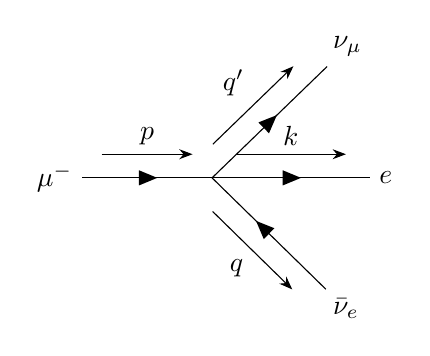
\begin{tikzpicture}
    \begin{feynman}
      \vertex (l) {$\mu^-$};
      \vertex [right=2cm of l] (c);
      \vertex [above right=2cm of c] (tr) {$\nu_\mu$};
      \vertex [right=2cm of c] (r) {$e$};
      \vertex [below right=2cm of c] (br) {$\bar{\nu}_e$};
      \diagram*{
        (l) -- [fermion, momentum=$p$] (c) -- [fermion, momentum=$k$] (r),
        (c) -- [anti fermion, momentum'=$q$] (br),
        (c) -- [fermion, momentum=$q'$] (tr),
      };
    \end{feynman}
  \end{tikzpicture}
\end{center}
We will make the simplifying assumption that neutrinos are massless.

The relevant bit of $\mathcal{L}_W^{\mathrm{eff}}$ is
\[
  - \frac{G_F}{\sqrt{2}} J^{\alpha\dagger}J_\alpha,
\]
where the weak current is
\[
  J^\alpha = \bar{\nu}_e \gamma^\alpha (1 - \gamma^5) e + \bar{\nu}_\mu \gamma^\alpha(1 - \gamma^5)\mu + \bar{\nu}_\tau \gamma^\alpha(1 - \gamma^5) \tau.
\]
We see it is the interaction of the first two terms that will render this decay possible.

To make sure our weak field approximation is valid, we need to make sure we live in sufficiently low energy scales. The most massive particle involved is
\[
  m_\mu = \SI{105.6583715(35)}{\mega\electronvolt}.
\]
On the other hand, the mass of the weak boson is
\[
  m_W = \SI{80.385(15)}{\giga\electronvolt},
\]
which is much bigger. So the weak field approximation should be valid.

We can now compute
\[
  M = \brak{e^-(k) \bar{\nu}_e (q) \nu_\mu(q')} \mathcal{L}_W^{\mathrm{eff}} \bket{\mu^-(p)}.
\]
Note that we left out all the spin indices to avoid overwhelming notation. We see that the first term in $J^\alpha$ is relevant to the electron bit, while the second is relevant to the muon bit. We can then write this as
\begin{align*}
  M &= -\frac{G_F}{\sqrt{2}} \brak{e^-(k) \bar{\nu}_e(q)} \bar{e} \gamma^\alpha (1 - \gamma^5) \nu_e \bket{0} \brak{\nu_\mu(q')} \bar{\nu}_\mu \gamma_\alpha(1 - \gamma^5) \mu \bket{\mu^-(p)}\\
  &= - \frac{G_F}{\sqrt{2}} \bar{u}_e(k) \gamma^\alpha (1 - \gamma^5)v_{\nu_e}(q) \bar{u}_{\nu_\mu} (q') \gamma_\alpha (1 - \gamma^5) u_p(p).
\end{align*}
Before we plunge through more computations, we look at what we are interested in and what we are not.

At this point, we are not interested in the final state spins. Therefore, we want to sum over the final state spins. We also don't know the initial spin of $\mu^-$. So we average over the initial states. For reasons that will become clear later, we will write the desired amplitude as
\begin{align*}
  \frac{1}{2} \sum_{\mathrm{spins}} |M|^2 &= \frac{1}{2} \sum_{\mathrm{spins}} MM^*\\
  &= \frac{1}{2} \frac{G_F^2}{2} \sum_{\mathrm{spins}} \left(\bar{u}_e(k) \gamma^\alpha (1 - \gamma^5) v_{\nu_e}(q)\bar{u}_{\nu_\mu} (q') \gamma_\alpha (1 - \gamma^5) u_\mu(p)\right)\\
  &\hphantom{\frac{1}{2} \frac{G_F^2}{2}\sum_{\mathrm{spins}}}\times \left(\bar{u}_\mu (p) \gamma_\beta(1 - \gamma^5) u_{\nu_\mu}(q') \bar{v}_{\nu_e}(q) \gamma^\beta (1 - \gamma^5) u_e(k)\right)\\
  &= \frac{1}{2} \frac{G_F^2}{2} \sum_{\mathrm{spins}} \left(\bar{u}_e(k) \gamma^\alpha (1 - \gamma^5) v_{\nu_e}(q) \bar{v}_{\nu_e}(q) \gamma^\beta (1 - \gamma^5) u_e(k)\right)\\
  &\hphantom{\frac{1}{2} \frac{G_F^2}{2}\sum_{\mathrm{spins}}}\times \left(\bar{u}_{\nu_\mu} (q') \gamma_\alpha (1 - \gamma^5) u_\mu(p) \bar{u}_\mu (p) \gamma_\beta(1 - \gamma^5) u_{\nu_\mu}(q')\right).
\end{align*}
We write this as
\[
  \frac{G_F^2}{4} S_1^{\alpha\beta}S_{2\alpha\beta},
\]
where
\begin{align*}
  S_1^{\alpha\beta} &= \sum_{\mathrm{spins}} \bar{u}_e(k) \gamma^\alpha (1 - \gamma^5) v_{\nu_e}(q) \bar{v}_{\nu_e}(q) \gamma^\beta (1 - \gamma^5) u_e(k)\\
  S_{2\alpha\beta} &= \sum_{\mathrm{spins}}\bar{u}_{\nu_\mu} (q') \gamma_\alpha (1 - \gamma^5) u_\mu(p) \bar{u}_\mu (p) \gamma_\beta(1 - \gamma^5) u_{\nu_\mu}(q').
\end{align*}
To actually compute this, we recall the spinor identities
\begin{align*}
  \sum_{\mathrm{spins}} u(p) \bar{u}(p) &= \slashed{p} + m,\\
  \sum_{\mathrm{spins}} v(p) \bar{v}(p) &= \slashed{p} - m
\end{align*}
In our expression for, say, $S_1$, the $v_{\nu_e} \bar{v}_{\nu_e}$ is already in the right form to apply these identities, but $\bar{u}_e$ and $u_e$ are not. Here we do a slightly sneaky thing. We notice that for each fixed $\alpha, \beta$, the quantity $S^{\alpha\beta}_1$ is a scalar. So we trivially have $S_1^{\alpha\beta} = \Tr(S_1^{\alpha \beta})$. We now use the cyclicity of trace, which says $\Tr (AB) = \Tr (BA)$. This applies even if $A$ and $B$ are not square, by the same proof. Then noting further that the trace is linear, we get
\begin{align*}
  S_1^{\alpha\beta} &= \Tr(S_1^{\alpha\beta}) \\
  &= \sum_{\mathrm{spins}} \Tr \Big[\bar{u}_e(k) \gamma^\alpha (1 - \gamma^5) v_{\nu_e}(q) \bar{v}_{\nu_e}(q) \gamma^\beta (1 - \gamma^5)\Big]\\
  &= \sum_{\mathrm{spins}} \Tr \Big[u_e(k)\bar{u}_e(k) \gamma^\alpha (1 - \gamma^5) v_{\nu_e}(q) \bar{v}_{\nu_e}(q) \gamma^\beta (1 - \gamma^5)\Big]\\
  &= \Tr \Big[(\slashed{k} + m_e) \gamma^\alpha (1 - \gamma^5) \slashed{q} \gamma^\beta(1 - \gamma^5)\Big]\\
  \intertext{Similarly, we find}
  S_{2\alpha\beta} &= \Tr \Big[\slashed{q}' \gamma_\alpha(1 - \gamma^5) (\slashed{p} + m_\mu) \gamma_\beta(1 - \gamma^5)\Big].
\end{align*}
To evaluate these traces, we use trace identities
\begin{align*}
  \Tr(\gamma^{\mu_1} \cdots \gamma^{\mu_n}) &= 0\text{ if $n$ is odd}\\
  \Tr(\gamma^\mu \gamma^\nu \gamma^\rho \gamma^\sigma) &= 4 (g^{\mu\nu} g^{\rho\sigma} - g^{\mu\rho} \gamma^{\nu\sigma} + g^{\mu\sigma} g^{\nu\rho})\\
  \Tr(\gamma^5 \gamma^\mu \gamma^\nu \gamma^\rho \gamma^\sigma) &= 4i \varepsilon^{\mu\nu\rho\sigma}.
\end{align*}
This gives the rather scary expressions
\begin{align*}
  S_1^{\alpha\beta} &= 8\Big(k^\alpha q^\beta + k^\beta q^\alpha - (k\cdot q) g^{\alpha\beta} - i \varepsilon^{\alpha\beta\mu\rho} k_\mu q_\rho\Big)\\
  S_{2\alpha\beta} &= 8\Big(q'_\alpha p_\beta + q'_\beta p_\alpha - (q' \cdot p) g_{\alpha\beta} - i \varepsilon_{\alpha\beta\mu\rho} q'^\mu p^\rho\Big),
\end{align*}
but once we actually contract these two objects, we get the really pleasant result
\[
  \frac{1}{2} \sum |M|^2 = 64 G_F^2 (p \cdot q)(k \cdot q').
\]
It is instructive to study this expression in particular cases. Consider the case where $e^-$ and $\nu_\mu$ go out along the $+z$ direction, and $\bar{\nu}_e$ along $-z$. Then we have
\[
  k \cdot q' = \sqrt{m_e^2 + k_z^2} q_z' - k_z q'_z.
\]
As $m_e \to 0$, we have $\to 0$.

This is indeed something we should expect even without doing computations. We know weak interaction couples to left-handed particles and right-handed anti-particles. \emph{If} $m_e = 0$, then we saw that helicity are chirality the same. Thus, the spin of $\bar{\nu}_e$ must be opposite to that of $\nu_\mu$ and $e^-$:
\begin{center}
  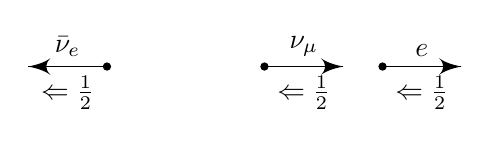
\begin{tikzpicture}
    \node [circ] {};
    \draw [->] (0, 0) -- (-1, 0) node [pos=0.5, above] {$\bar{\nu}_e$} node [pos=0.5, below] {$\Leftarrow \frac{1}{2}$};

    \node [circ] at (2, 0) {};
    \draw [->] (2, 0) -- (3, 0) node [pos=0.5, above] {$\nu_\mu$} node [pos=0.5, below] {$\Leftarrow \frac{1}{2}$};

    \node [circ] at (3.5, 0) {};
    \draw [->] (3.5, 0) -- (4.5, 0) node [pos=0.5, above] {$e$} node [pos=0.5, below] {$\Leftarrow \frac{1}{2}$};
  \end{tikzpicture}
\end{center}
So they all point in the same direction, and the total spin would be $\frac{3}{2}$. But the initial total angular momentum is just the spin $\frac{1}{2}$. So this violates conservation of angular momentum.

But if $m_e \not= 0$, then the left-handed and right-handed components of the electron are coupled, and helicity and chirality do not coincide. So it is possible that we obtain a right-handed electron instead, and this gives conserved angular momentum. We call this \term{helicity suppression}, and we will see many more examples of this later on.

It is important to note that here we are only analyzing decays where the final momenta point in these particular directions. If $m_e = 0$, we can still have decays in other directions.

There is another interesting thing we can consider. In this same set up, if $m_e \not= 0$, but neutrinos are massless, then we can only possibly decay to left-handed neutrinos. So the only possible assignment of spins is this:
\begin{center}
  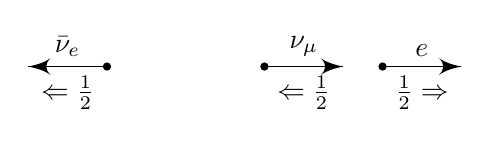
\begin{tikzpicture}
    \node [circ] {};
    \draw [->] (0, 0) -- (-1, 0) node [pos=0.5, above] {$\bar{\nu}_e$} node [pos=0.5, below] {$\Leftarrow \frac{1}{2}$};

    \node [circ] at (2, 0) {};
    \draw [->] (2, 0) -- (3, 0) node [pos=0.5, above] {$\nu_\mu$} node [pos=0.5, below] {$\Leftarrow \frac{1}{2}$};

    \node [circ] at (3.5, 0) {};
    \draw [->] (3.5, 0) -- (4.5, 0) node [pos=0.5, above] {$e$} node [pos=0.5, below] {$\frac{1}{2} \Rightarrow$};
  \end{tikzpicture}
\end{center}
Under parity transform, the momenta reverse, but spins don't. If we transform under parity, we would expect to see the same behaviour.
\begin{center}
  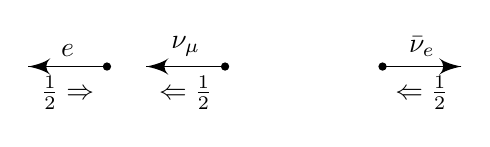
\begin{tikzpicture}[xscale=-1]
    \node [circ] {};
    \draw [->] (0, 0) -- (-1, 0) node [pos=0.5, above] {$\bar{\nu}_e$} node [pos=0.5, below] {$\Leftarrow \frac{1}{2}$};

    \node [circ] at (2, 0) {};
    \draw [->] (2, 0) -- (3, 0) node [pos=0.5, above] {$\nu_\mu$} node [pos=0.5, below] {$\Leftarrow \frac{1}{2}$};

    \node [circ] at (3.5, 0) {};
    \draw [->] (3.5, 0) -- (4.5, 0) node [pos=0.5, above] {$e$} node [pos=0.5, below] {$\frac{1}{2} \Rightarrow$};
  \end{tikzpicture}
\end{center}
But (at least in the limit of massless neutrinos) this isn't allowed, because weak interactions don't couple to right-handed neutrinos. So we know that weak decays violate P.

We now now return to finish up our computations. The decay rate is given by
\begin{multline*}
  \Gamma = \frac{1}{2 m_\mu} \int \frac{\d^3 k}{(2\pi)^3 2k^0} \int \frac{\d^3 q}{(2\pi)^3 2q^0} \int \frac{\d^3 q'}{(2\pi)^3 q'^0} \\
  \times (2\pi)^4 \delta^{(4)}(p - k - q - q') \frac{1}{2} \sum |M|^2.
\end{multline*}
Using our expression for $|M|$, we find
\[
  \Gamma = \frac{G_F^2}{8 \pi^5 m_\mu} \int \frac{\d^3 k\; \d^3 q\; \d^3 q'}{k^0 q^0 q'^0} \delta^{(4)} (p - k - q - q') (p \cdot q) (k \cdot q').
\]
To evaluate this integral, there is a useful trick.

For convenience, we write $Q = p - k$, and we consider
\[
  I_{\mu\nu}(Q) = \int \frac{\d^3 q}{q^0} \frac{\d^3 q'}{q'^0} \delta^{(4)}(Q - q - q') q_\mu q'_\nu.
\]
By Lorentz symmetry arguments, this must be of the form
\[
  I_{\mu\nu} (Q) = a(Q^2) Q_\mu Q_\nu + b(Q^2) g_{\mu\nu} Q^2,
\]
where $a, b: \R \to \R$ are some scalar functions.

Now consider
\[
  g^{\mu\nu} I_{\mu\nu} = \int \frac{\d^3 q}{q^0} \frac{\d^3 q'}{q'^0} \delta^{(4)}(Q - q - q') q \cdot q' = (a + 4b) Q^2 .
\]
But we also know that
\[
  (q + q')^2 = q^2 + q'^2 + 2 q \cdot q' = 2 q \cdot q'
\]
because neutrinos are massless. On the other hand, by momentum conservation, we know
\[
  q + q' = Q.
\]
So we know
\[
  q \cdot q' = \frac{1}{2} Q^2.
\]
So we find that
\[
  a + 4b = \frac{I}{2},\tag{$1$}
\]
where
\[
  I = \int \frac{\d^3 q}{q^0} \int \frac{\d^3 q'}{q'^0} \delta^{(4)} (Q - q - q').
\]
We can consider something else. We have
\begin{multline*}
  Q^\mu Q^\nu I_{\mu\nu} = a(Q^2) Q^4 + b(Q^2) Q^4 \\
  = \int \frac{\d^3 q}{q^0} \int \frac{\d^3 q'}{q'^0} \delta^{(4)} (Q - q - q') (q\cdot Q) (q' \cdot Q).
\end{multline*}
Using the masslessness of neutrinos and momentum conservation again, we find that
\[
  (q \cdot Q) (q' \cdot Q) = (q \cdot q') (q \cdot q').
\]
So we find
\[
  a + b = \frac{I}{4}\tag{$2$}.
\]
It remains to evaluate $I$, and to do so, we can just evaluate it in the frame where $Q = (\sigma, 0)$ for some $\sigma$. Now note that since $q^2 = q'^2 = 0$, we must have
\[
  q^0 = |\mathbf{q}|.
\]
So we have
\begin{align*}
  I &= \int \frac{\d^3 q}{|\mathbf{q}|} \int \frac{\d^3 q'}{|\mathbf{q}'|} \delta(\sigma - |\mathbf{q}| - |\mathbf{q}'|) \prod_{i = 1}^3 \delta(q_i - q_i')\\
  &= \int \frac{\d^3 q}{|\mathbf{q}|^2} \delta(\sigma - 2|\mathbf{q}|)\\
  &= 4\pi \int_0^\infty \d |\mathbf{q}|\; \delta(\sigma - 2|\mathbf{q}|)\\
  &= 2\pi.
\end{align*}
So we find that
\[
  \Gamma = \frac{G_F^2}{3 m_\mu (2\pi)^4} \int \frac{\d^3 k}{k^0} \Big(2 p \cdot (p - k) k \cdot (p - k) + (p \cdot k)(p - k)^2\Big)
\]
Recall that we are working in the rest frame of $\mu$. So we know that
\[
  p \cdot k = m_\mu E,\quad p \cdot p = m_\mu^2,\quad k \cdot k = m_e^2,
\]
where $E = k^0$. Note that we have
\[
  \frac{m_e}{m_\mu}\approx 0.0048 \ll 1.
\]
So to make our lives easier, it is reasonable to assume $m_e = 0$. In this case, $|\mathbf{k}| = E$, and then
\begin{align*}
  \Gamma &= \frac{G_F^2}{(2\pi)^4 3m_\mu} \int \frac{\d^3 k}{E} \Big(2 m_\mu^2 m_\mu E - 2 (m_\mu E)^2 - 2 (m_\mu E)^2 + m_\mu E m_\mu^2\Big)\\
  &= \frac{G_F^2 m_\mu}{ (2\pi)^4 3} \int \d^3 k\; (3 m_\mu - 4 E)\\
  &= \frac{4\pi G_F^2 m_\mu}{(2\pi)^4 3} \int \d E\; E^2(3 m_\mu - 4E)
\end{align*}
We now need to figure out what we want to integrate over. When $e$ is at rest, then $E_{\mathrm{min}} = 0$. The maximum energy is obtained when $\nu_\mu, \bar{\nu}_e$ are in the same direction and opposite to $e^-$. In this case, we have
\[
  E + (E_{\bar{\nu}_e} + E_{\nu_\mu}) = m_\mu.
\]
By energy conservation, we also have
\[
  E - (E_{\bar{\nu}_e} + E_{\nu_\mu}) = 0.
\]
So we find
\[
  E_{\mathrm{max}} = \frac{m_\mu}{2}.
\]
Thus, we can put in our limits into the integral, and find that % figure out where the limits come from. What happens when we integrate past this limit?
\[
  \Gamma = \frac{G_F^2 m_\mu^5}{192 \pi^3}.
\]
As we mentioned at the beginning of the chapter, this is the only decay channel off the muon. From experiments, we can measure the lifetime of the muon as
\[
  \tau_{\mu} = \SI{2.1870e-6}{\second}.
\]
This tells us that
\[
  G_F = \SI{1.164e-5}{\giga\electronvolt\squared}.
\]
Of course, this isn't exactly right, because we ignored all loop corrections (and approximated $m_e = 0$). But this is reasonably good, because those effects are very small, at an order of $10^{-6}$ as large. Of course, if we want to do more accurate and possibly beyond standard model physics, we need to do better than this.

Experimentally, $G_F$ is consistent with what we find in the $\tau \to e \bar{\nu}_e \nu_\tau$ and $\mu \to e \bar{\nu}_e \nu_\mu$ decays. This is some good evidence for lepton universality, i.e.\ they have different masses, but they couple in the same way.

\subsection{Pion decay}
We are now going to look at a slightly different example. We are going to study decays of \term{pions}, which are made up of a pair of quark and anti-quark. We will in particular look at the decay
\[
  \pi^- (\bar u d) \to e^- \bar{\nu}_e.
\]
\begin{center}
  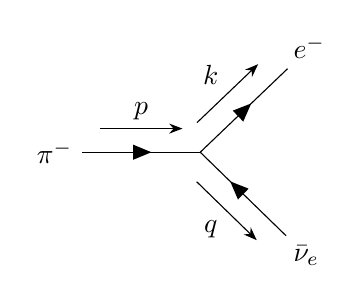
\begin{tikzpicture}
    \begin{feynman}
      \vertex (c);
      \vertex [left=of c] (pi) {$\pi^-$};
      \vertex [above right=of c] (e) {$e^-$};
      \vertex [below right=of c] (nu) {$\bar{\nu}_e$};

      \diagram*{
        (pi) -- [fermion, momentum=$p$] (c) -- [fermion, momentum=$k$] (e);
        (c) -- [anti fermion, momentum'=$q$] (nu);
      };
    \end{feynman}
  \end{tikzpicture}
\end{center}
This is actually quite hard to do from first principles, because $\pi^-$ is made up of quarks, and quark dynamics is dictated by QCD, which we don't know about yet. However, these quarks are not free to move around, and are strongly bound together inside the pion. So the trick is to hide all the things that happen in the QCD side in a single constant $F_\pi$, without trying to figure out, from our theory, what $F_\pi$ actually is.

The relevant currents are
\begin{align*}
  J_{\mathrm{lept}}^\alpha &= \bar{\nu}_e \gamma^\alpha (1 - \gamma^5) e\\
  J_{\mathrm{had}}^\alpha &= \bar{u} \gamma^\alpha (1 - \gamma^5)(V_{ud} d + V_{us}s + v_{ub}b) \equiv V_{\mathrm{had}}^\alpha - A_{\mathrm{had}}^\alpha,
\end{align*}
where the $V_{\mathrm{had}}^\alpha$ contains the $\gamma^\alpha$ bit, while $A_{\mathrm{had}}^\alpha$ contains the $\gamma^\alpha \gamma^5$ bit.

Then the amplitude we want to compute is
\begin{align*}
  M &= \brak{e^-(k) \bar{\nu}_e (q)} \mathcal{L}_W^{\mathrm{eff}} \bket{\pi^-(p)}\\
  &= - \frac{G_F}{\sqrt{2}} \brak{e^-(k) \bar{\nu}_e(q)} J_{\alpha, \mathrm{lept}}^\dagger \bket{0} \brak{0} J_{\mathrm{had}}^\alpha \bket{\pi^-(p)}\\
  &= - \frac{G_F}{\sqrt{2}} \brak{e^-(k) \bar{\nu}_e(q)} \bar{e} \gamma_\alpha (1 - \gamma^5) \nu_e \bket{0} \brak{0} J_{\mathrm{had}}^\alpha \bket{\pi^-(p)}\\
  &= \frac{G_F}{\sqrt{2}} \bar{u}_e (k) \gamma_\alpha(1 - \gamma^5) v_{\nu_e}(q) \brak{0} V_{\mathrm{had}}^\alpha - A_{\mathrm{had}}^\alpha \bket{\pi^-(p)}.
\end{align*}
We now note that $V_{\mathrm{had}}^\alpha$ does not contribute. This requires knowing something about QCD and $\pi^-$. It is known that QCD is a P-invariant theory, and experimentally, we find that $\pi^-$ has spin $0$ and odd parity. In other words, under P, it transforms as a pseudoscalar. Thus, the expression
\[
  \brak{0}\bar{u} \gamma^\alpha d \bket{\pi^-(p)}
\]
transforms as an axial vector. But since the only physical variable involved is $p^\alpha$, the only quantities we can construct are multiples of $p^\alpha$, which are vectors. So this must vanish. By a similar chain of arguments, the remaining part of the QCD part must be of the form
\[
  \brak{0} \bar{u} \gamma^\alpha \gamma^5 d \bket{\pi^-(p)} = i \sqrt{2} F_\pi p^\alpha
\]
for some constant \term{$F_\pi$}. Then we have
\[
  M = i G_F F_\pi V_{ud} \bar{u}_e(k) \slashed p (1 - \gamma^5) v_{\nu_e}(q).
\]
To simplify this, we use momentum conservation $p = k + q$, and some spinor identities
\[
  \bar{u}_e(k) \slashed{k} = \bar{u}_e(k) m_e,\quad \slashed{q} v_{\nu_e}(q) = 0.
\]
Then we find that
\[
  M = i G_F F_\pi V_{ud} m_e \bar{u}_e(k) (1 - \gamma^5) v_{\nu_e}(q).
\]
Doing a manipulation similar to last time's, and noting that
\begin{align*}
  (1 - \gamma^5) \gamma^\mu(1 + \gamma^5) &= 2(1 - \gamma^5) \gamma^\mu\\
  \Tr (\slashed{k}\slashed{q}) &= 4 k\cdot q\\
  \Tr (\gamma^5 \slashed{k}\slashed{q}) &= 0
\end{align*}
we find
\begin{align*}
  \sum_{\text{spins }e, \bar{\nu}_e} |M|^2 &= \sum_{\mathrm{spins}} |G_F F_\pi m_e V_{ud}|^2 [\bar{u}_e(k) (1 - \gamma^5) v_{\nu_e}(q) \bar{v}_{\nu_e}(q) (1 + \gamma^5) u_e(k)]\\
  &= 2|G_F F_\pi m_e V_{ud}|^2 \Tr \Big[(\slashed{k} + m_e)( 1 - \gamma^5) \slashed{q}\Big]\\
  &= 8 |G_F F_\pi m_e V_{ud}|^2 (k \cdot q).
\end{align*}
This again shows helicity suppression. The spin-$0$ $\pi^-$ decays to the positive helicity $\bar{\nu}_e$, and hence decays to a positive helicity electron by helicity conservation.
\begin{center}
  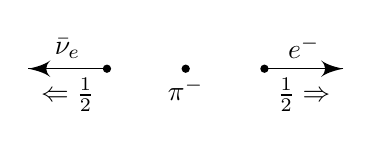
\begin{tikzpicture}
    \node [circ] {};
    \node [below] at (0, 0) {$\pi^-$};

    \draw [->] (1, 0) node [circ] {} -- (2, 0) node [pos=0.5, above] {$e^-$} node [pos=0.5, below] {$\frac{1}{2} \Rightarrow$};
    \draw [->] (-1, 0) node [circ] {} -- (-2, 0) node [pos=0.5, above] {$\bar{\nu}_e$} node [pos=0.5, below] {$\Leftarrow \frac{1}{2}$};
  \end{tikzpicture}
\end{center}
But if $m_e = 0$, then this has right-handed chirality, and so this decay is forbidden.

We can now compute an actual decay rate. We note that since we are working in the rest frame of $\pi^-$, we have $\mathbf{k} + \mathbf{q} = 0$; and since the neutrino is massless, we have $q^0 = |\mathbf{q}| = |\mathbf{k}|$. Finally, writing $E = k^0$ for the energy of $e^-$, we obtain
\begin{align*}
  \Gamma_{\pi \to e \bar{\nu}_e} &= \frac{1}{2 m_\pi} \int \frac{\d^3 k}{(2\pi)^3 2 k^0} \int \frac{\d^3 q}{(2\pi)^3 2 q^0} (2\pi)^4 \delta^{(4)}(p - k - q) \\
  &\hphantom{aaaaaaaaaaaaaaaaaaaaaaaaaaaaaaaa} 8 |G_F F_\pi m_e V_{ud}|^2 (k \cdot q)\\
  &= \frac{|G_F F_\pi m_e V_{ud}|^2 }{4 m_\pi \pi^2} \int \frac{\d^3 k}{E|\mathbf{k}|} \delta(m_{\pi} - E - |\mathbf{k}|) (E |\mathbf{k}| + |\mathbf{k}|^2)
\end{align*}
To simplify this further, we use the property
\[
  \delta(f(k)) = \sum_i \frac{\delta(k - k_0^i)}{|f'(k_0^i)|},
\]
where $k_0^i$ runs over all roots of $f$. In our case, we have a unique root
\[
  k_0 =\frac{m_\pi^2 - m_e^2}{2m_\pi},
\]
and the corresponding derivative is
\[
  |f'(k_0)| = 1 + \frac{k_0}{E}.
\]
Then we get
\begin{align*}
  \Gamma_{\pi \to e \bar{\nu}_e} &= \frac{|G_F F_\pi m_e V_{ud}|^2}{4 \pi^2 m_\pi}\int \frac{4\pi k^2 \;\d k}{E} \frac{E + k}{1 + k_0/E} \delta(k - k_0)\\
  &= \frac{|G_F F_\pi V_{ud}|^2}{4\pi} m_e^2 m_\pi \left(1 - \frac{m_e^2}{m_\pi^2}\right)^2.
\end{align*}
Note that if we set $m_e \to 0$, then this vanishes. This time, it is the whole decay rate, and not just some particular decay channel.

Let's try to match this with experiment. Instead of looking at the actual lifetime, we compare it with some other possible decay rates. The expression for $\Gamma_{\pi \to \mu \bar{\nu}_\mu}$ is exactly the same, with $m_e$ replaced with $m_\mu$. So the ratio
\[
  \frac{\Gamma_{\pi \to e\bar{\nu}_e}}{\Gamma_{\pi \to \mu \bar{\nu}_\mu}} = \frac{m_e^2}{m_\mu^2} \left(\frac{m_\pi^2 - m_e^2}{m_\pi^2 - m_\mu^2}\right)^2 \approx 1.28 \times 10^{-4}.
\]
Here all the decay constants cancel out. So we can actually compare this with experiment just by knowing the electron and muon masses. When we actually do experiments, we find $1.230(4) \times 10^{-4}$. This is pretty good agreement, but not agreement to within experimental error. Of course, this is not unexpected, because we didn't include the quantum loop effects in our calculations.

Another thing we can see is that the ratio is very small, on the order of $10^{-4}$. This we can understand from helicity suppression, because $m_\mu \gg m_e$.

Note that we were able to get away without knowing how QCD works!

\subsection{\tph{$K^0\mdash \bar{K}^0$}{K0-K0}{K<sup>0</sup>-K<sup>0</sup>} mixing}
We now move on to consider our final example of weak decays, and look at $K^0$-$\bar{K}^0$ mixing. We will only do this rather qualitatively, and look at the effects of CP violation.

\term{Kaons} contain a strange quark/antiquark. There are four ``flavour eigenstates'' given by
\[
  K^0 (\bar{s} d),\quad \bar{K}^0 (\bar{d} s),\quad K^+(\bar{s} u),\quad K^-(\bar{u} s).
\]
These are the lightest kaons, and they have spin $J = 0$ and parity $p = -\mathrm{ve}$. We can concisely write these information as $J^p = 0^-$. These are pseudoscalars.

We want to understand how these things transform under CP. Parity transformation doesn't change the particle contents, and charge conjugation swaps particles and anti-particles. Thus, we would expect CP to send $K^0$ to $\bar{K}^0$, and vice versa. For kaons at rest, we can pick the relative phases such that
\begin{align*}
  \hat{C} \hat{P} \bket{K^0} &= - \bket{\bar{K}^0}\\
  \hat{C} \hat{P} \bket{\bar{K}^0} &= - \bket{K^0}.
\end{align*}
So the CP eigenstates are just
\[
  \bket{K_\pm^0} = \frac{1}{\sqrt{2}} (\bket{K^0} \mp \bket{\bar{K}^0}).
\]
Then we have
\[
  \hat{C}\hat{P} \bket{K_{\pm}^0} = \pm \bket{K_{\pm}^0}.
\]
Let's consider the two possible decays $K^0 \to \pi^0 \pi^0$ and $K^0 \to \pi^+ \pi^-$. This requires converting one of the strange quarks into an up or down quark.
\begin{center}
  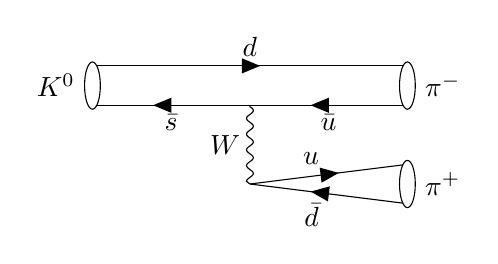
\begin{tikzpicture}
    \begin{feynman}
      \vertex (tl);
      \vertex [below=0.5cm of tl] (bl);
      \vertex [right=2cm of bl] (bc);
      \vertex [right=2cm of bc] (br);
      \vertex [above=0.5cm of br] (tr);

      \vertex [below=1cm of bc] (d);

      \vertex [right=2cm of d] (r);
      \vertex [above=0.25cm of r] (ru);
      \vertex [below=0.25cm of r] (rd);

      \diagram*{
        (tl) -- [fermion, edge label=$d$] (tr),
        (bl) -- [anti fermion, edge label'=$\bar{s}$] (bc),
        (bc) -- [anti fermion, edge label'=$\bar{u}$] (br),
        (bc) -- [photon, edge label'=$W$] (d),
        (d) -- [fermion, edge label=$u$] (ru),
        (d) -- [anti fermion, edge label'=$\bar{d}$] (rd),
      };
    \end{feynman}

    \draw [fill=white] (0, -0.25) ellipse (0.1 and 0.3); % make this more beautiful
    \node [left] at (-0.1, -0.25) {$K^0$};

    \draw [fill=white] (4, -0.25) ellipse (0.1 and 0.3);
    \node [right] at (4.1, -0.25) {$\pi^-$};

    \draw [fill=white] (4, -1.5) ellipse (0.1 and 0.3);
    \node [right] at (4.1, -1.5) {$\pi^+$};
  \end{tikzpicture}
\end{center}
\begin{center}
  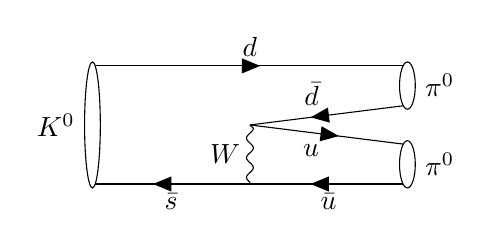
\begin{tikzpicture}
    \begin{feynman}
      \vertex at (0, 0) (tl);
      \vertex at (4, 0) (r1);
      \vertex at (4, -0.5) (r2);
      \vertex at (4, -1) (r3);
      \vertex at (4, -1.5) (r4);
      \vertex at (0, -1.5) (bl);
      \vertex at (2, -1.5) (bc);
      \vertex at (2, -0.75) (c);
      \diagram*{
        (tl) -- [fermion, edge label=$d$] (r1),
        (bl) -- [anti fermion, edge label'=$\bar{s}$] (bc) -- [anti fermion, edge label'=$\bar{u}$] (r4),
        (bc) -- [photon, edge label=$W$] (c),
        (c) -- [anti fermion, edge label=$\bar{d}$] (r2),
        (c) -- [fermion, edge label'=$u$] (r3)
      };
    \end{feynman}

    \draw [fill=white] (0, -0.75) ellipse (0.1 and 0.8); % make this more beautiful
    \node [left] at (-0.1, -0.75) {$K^0$};

    \draw [fill=white] (4, -0.25) ellipse (0.1 and 0.3);
    \node [right] at (4.1, -0.25) {$\pi^0$};

    \draw [fill=white] (4, -1.25) ellipse (0.1 and 0.3);
    \node [right] at (4.1, -1.25) {$\pi^0$};
  \end{tikzpicture}
\end{center}
From the conservation of angular momentum, the total angular momentum of $\pi \pi$ is zero. Since they are also spinless, the orbital angular momentum $L = 0$.

When we apply CP to the final states, we note that the relative phases of $\pi^+$ and $\pi^-$ (or $\pi^0$ and $\pi^0$) cancel out each other. So we have
\[
  \hat{C}\hat{P} \bket{\pi^+\pi^-} = (-1)^L \bket{\pi^+\pi^-} = \bket{\pi^+ \pi^-},
\]
where the relative phases of $\pi^+$ and $\pi^-$ cancel out. Similarly, we have
\[
  \hat{C}\hat{P} \bket{\pi^0 \pi^0} = \bket{\pi^0 \pi^0}.
\]
Therefore $\pi \pi$ is always a CP eigenstate with eigenvalue $+1$.

What does this tell us about the possible decays? We know that CP is conserved by the strong and electromagnetic interactions. If it were conserved by the weak interaction as well, then there is a restriction on what can happen. We know that
\[
  K^0_+ \to \pi \pi
\]
is allowed, because both sides have CP eigenvalue $+1$, but
\[
  K^0_- \to \pi \pi
\]
is not. So $K^0_+$ is ``short-lived'', and $K^0_-$ is ``long-lived''. Of course, $K^0_-$ will still decay, but must do so via more elaborate channels, e.g.\ $K^0_- \to \pi \pi \pi$.

Does this agree with experiments? When we actually look at Kaons, we find two neutral Kaons, which we shall call $K^0_S$ and $K_L^0$. As the subscripts suggest, $K^0_S$ has a ``short'' lifetime of $\tau \approx \SI{9e-11}{\second}$, while $K^0_L$ has a ``long'' lifetime of $\tau \approx \SI{5e-8}{\second}$.

But does this actually CP is not violated? Not necessarily. For us to be correct, we want to make sure $K_L^0$ never decays to $\pi\pi$. We define the quantities
\[
  \eta_{+ -} = \frac{|\brak{\pi^+ \pi^-}H \bket{K_L^0}|}{|\brak{\pi^+ \pi^-}H \bket{K_S^0}|},\quad \eta_{0 0} = \frac{|\brak{\pi^0 \pi^0}H \bket{K_L^0}|}{|\brak{\pi^0 \pi^0}H \bket{K_S^0}|}
\]
Experimentally, when we measure these things, we have
\[
  \eta_{\pm} \approx \eta_{00} \approx 2.2\times 10^{-3} \not= 0.
\]
So $K_L^0$ does decay into $\pi \pi$.

If we think about what is going on here, there are two ways CP can be violated:
\begin{itemize}
  \item Direct CP violation of $s \to u$ due to a phase in $V_{CKM}$. % what is this?
  \item Indirect CP violation due to $K^0 \to \bar{K}^0$ or vice-versa, then decaying.
\end{itemize}
Of course, ultimately, the ``indirect violation'' is still due to phases in the CKM matrix, but the second is more ``higher level''.

It turns out in this particular process, it is the indirect CP violation that is mainly responsible, and the dominant contributions are ``box diagrams'', where the change in strangeness $\Delta S = 2$.
\begin{center}
  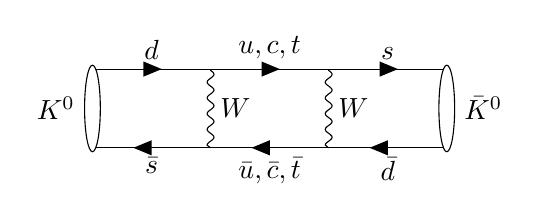
\begin{tikzpicture}
    \begin{feynman}
      \vertex (ull);
      \vertex (ul) [right=of ull];
      \vertex (ur) [right=of ul];
      \vertex (urr) [right=of ur];

      \vertex (dll) [below=1cm of ull];
      \vertex (dl) [right=of dll];
      \vertex (dr) [right=of dl];
      \vertex (drr) [right=of dr];

      \diagram*{
        (ull) -- [fermion, edge label=$d$] (ul) -- [fermion, edge label={$u, c, t$}] (ur) -- [fermion, edge label=$s$] (urr),
        (dll) -- [anti fermion, edge label'=$\bar{s}$] (dl) -- [anti fermion, edge label'={$\bar{u}, \bar{c}, \bar{t}$}] (dr) -- [anti fermion, edge label'=$\bar{d}$] (drr),
        (ul) -- [photon, edge label=$W$] (dl),
        (ur) -- [photon, edge label=$W$] (dr),
      };
    \end{feynman}
    \draw [fill=white] (0, -0.5) ellipse (0.1 and 0.55); % make this more beautiful
    \node [left] at (-0.1, -0.5) {$K^0$};
    \draw [fill=white] (4.5, -0.5) ellipse (0.1 and 0.55); % make this more beautiful
    \node [right] at (4.6, -0.5) {$\bar K^0$};
  \end{tikzpicture}
\end{center}
\begin{center}
  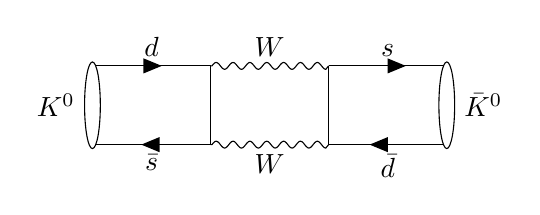
\begin{tikzpicture}
    \begin{feynman}
      \vertex (ull);
      \vertex (ul) [right=of ull];
      \vertex (ur) [right=of ul];
      \vertex (urr) [right=of ur];

      \vertex (dll) [below=1cm of ull];
      \vertex (dl) [right=of dll];
      \vertex (dr) [right=of dl];
      \vertex (drr) [right=of dr];

      \diagram*{
        (ull) -- [fermion, edge label=$d$] (ul) -- (dl) -- [fermion, edge label=$\bar{s}$] (dll),
        (urr) -- [anti fermion, edge label'=$s$] (ur) -- (dr) -- [anti fermion, edge label'=$\bar{d}$] (drr),
        (ul) -- [photon, edge label=$W$] (ur),
        (dl) -- [photon, edge label'=$W$] (dr),
      };
    \draw [fill=white] (0, -0.5) ellipse (0.1 and 0.55); % make this more beautiful
    \node [left] at (-0.1, -0.5) {$K^0$};
    \draw [fill=white] (4.5, -0.5) ellipse (0.1 and 0.55);
    \node [right] at (4.6, -0.5) {$\bar K^0$};
  \end{feynman}
  \end{tikzpicture}
\end{center}
Given our experimental results, we know that $K_S^0$ and $K_L^0$ aren't \emph{quite} $K_+^0$ and $K_-^0$ themselves, but have some corrections. We can write them as
\begin{align*}
  \bket{K_S^0} &= \frac{1}{\sqrt{1 + |\varepsilon_1|^2}} (\bket{K_+^0} + \varepsilon_1 \bket{K_-^0}) \approx \bket{K_+^0}\\
  \bket{K_L^0} &= \frac{1}{\sqrt{1 + |\varepsilon_2|^2}} (\bket{K_-^0} + \varepsilon_2 \bket{K_+^0}) \approx \bket{K_-^0},
\end{align*}
where $\varepsilon_1, \varepsilon_2 \in \C$ are some small complex numbers. This way, very occasionally, $K_L^0$ can decay as $K_+^0$.

We assume that we just have two state mixing, and ignore details of the strong interaction. Then as time progresses, we can write have
\begin{align*}
  \bket{K_S(t)} &= a_S(t) \bket{K^0} + b_S(t) \bket{\bar{K}^0}\\
  \bket{K_L(t)} &= a_L(t) \bket{K^0} + b_L(t) \bket{\bar{K}^0}
\end{align*}
for some (complex) functions $a_S, b_S, a_L, b_L$. Recall that Schr\"odinger's equation says
\[
  i \frac{\d}{\d t} \bket{\psi(t)} = H \bket{\psi(t)}.
\]
Thus, we can write
\[
  i \frac{\d}{\d t}
  \begin{pmatrix}
    a\\ b
  \end{pmatrix} =
  R
  \begin{pmatrix}
    a\\b
  \end{pmatrix},
\]
where
\[
  R =
  \begin{pmatrix}
    \brak{K^0}H' \bket{K^0} & \brak{K^0}H' \bket{\bar{K}^0}\\
    \brak{\bar{K}^0}H' \bket{K^0} & \brak{\bar{K}^0}H' \bket{\bar{K}^0}
  \end{pmatrix}
\]
and $H'$ is the next-to-leading order weak Hamiltonian. Because Kaons decay in finite time, we know $R$ is not Hermitian. By general linear algebra, we can always write it in the form
\[
  R = M - \frac{i}{2} \Gamma,
\]
where $M$ and $\Gamma$ are Hermitian. We call $M$ the \term{mass matrix}, and $\Gamma$ the \term{decay matrix}.

We are not going to actually compute $R$, but we are going to use the known symmetries to put some constraint on $R$. We will consider the action of $\Theta = \hat{C}\hat{P}\hat{T}$. The CPT theorem says observables should be invariant under conjugation by $\Theta$. So if $A$ is Hermitian, then $\Theta A \Theta^{-1} = A$. Now our $H'$ is not actually Hermitian, but as above, we can write it as
\[
  H' = A + i B,
\]
where $A$ and $B$ are Hermitian. Now noting that $\Theta$ is \emph{anti-unitary}, we have
\[
  \Theta H' \Theta^{-1} = A - iB = H'^\dagger.
\]
In the rest frame of a particle $\bar{K}^0$, we know $\hat{T} \bket{K^0} = \bket{K^0}$, and similarly for $\bar{K}^0$. So we have
\[
  \Theta \bket{\bar{K}^0} = - \bket{K^0},\quad \Theta \bket{K^0} = - \bket{\bar{K}^0},
\]
Since we are going to involve time reversal, we stop using bra-ket notation for the moment. We have
\begin{multline*}
  R_{11} = (K^0, H' K^0)
  = (\Theta^{-1}\Theta K^0, H' \Theta^{-1}\Theta K^0)
  = (\bar{K}^0, H'^\dagger \bar{K}^0)^*\\
  = (H' \bar{K}^0, \bar{K}^0)^*
  = (\bar K^0, H' \bar{K}^0)
  = R_{22}
\end{multline*}
Now \emph{if} $\hat{T}$ was a good symmetry (i.e.\ $\hat{C}\hat{P}$ is good as well), then a similar computation shows that
\[
  R_{12} = R_{21}.
\]
We can show that we in fact have % maybe insert this
\[
  \varepsilon_1 = \varepsilon_2 = \varepsilon = \frac{\sqrt{R_{21}} - \sqrt{R_{21}}}{\sqrt{R_{12}} + \sqrt{R_{21}}}.
\]
So if CP is conserved, then $R_{12} = R_{21}$, and therefore $\varepsilon_1 = \varepsilon_2 = \varepsilon = 0$.

Thus, we see that if we want to have mixing, then we must have $\varepsilon_1, \varepsilon_2 \not= 0$. So we need $R_{12} \not =R_{21}$. In other words, we must have CP violation!

One can also show that
\[
  \eta_{+-} = \varepsilon + \varepsilon',\quad \eta_{00} = \varepsilon - 2 \varepsilon',
\]
where $\varepsilon'$ measures the direct source of CP violation. By looking at these two modes of decay, we can figure out the values of $\varepsilon$ and $\varepsilon'$. Experimentally, we find
\[
  |\varepsilon| = (2.228 \pm 0.011) \times 10^{-3},
\]
and
\[
  \left|\frac{\varepsilon}{\varepsilon'}\right| = (1.66 \pm 0.23) \times 10^{-3}.
\]
As claimed, it is the indirect CP violation that is dominant, and the direct one is suppressed by a factor of $10^{-3}$.

Other decays can be used to probe $K_{L, S}^0$. For example, we can look at semi-leptonic decays. We can check that
\[
  K^0 \to \pi^- e^+ \nu_e
\]
is possible, while
\[
  K^0 \to \pi^+ e^- \bar{\nu}_e
\]
is not. $\bar{K}^0$ has the opposite phenomenon. To show these, we just have to try to write down diagrams for these events. % insert diagram

Now if CP is conserved, we'd expect the decay rates
\[
  \Gamma(K_{L, S}^0 \to \pi^- e^+ \nu_e) = \Gamma(K_{L, S}^0 \to \pi^+ e^- \bar{\nu}_e),
\]
since we expect $K_{L, S}$ to consist of the same amount of $K^0$ and $\bar{K}^0$.

We define
\[
  A_L = \frac{\Gamma(K_L^0 \to \pi^- e^+ \nu_e) - \Gamma(K_L^0 \to \pi^+ e^- \bar{\nu}_e)}{\Gamma(K_L^0 \to \pi^- e^+ \nu_e) + \Gamma(K_L^0 \to \pi^+ e^- \bar{\nu}_e)}.
\]
If this is non-zero, then we have evidence for CP violation. Experimentally, we find
\[
  A_L = (3.32 \pm 0.06) \times 10^{-3} \approx 2 \Re (\varepsilon).
\]
This is small, but certainly significantly non-zero.

% We can actually use CP violation to tell some aliens far far away what we mean by matter and anti-matter.

\section{Quantum chromodynamics (QCD)}
In the early days of particle physics, we didn't really know what we were doing. So we just smashed particles into each other and see what happened. Our initial particle accelerators weren't very good, so we mostly observed some low energy particles.

Of course, we found electrons, but the more interesting discoveries were in the hadrons. We had protons and neutrons, $n$ and $p$, as well as pions $\pi^+, \pi^0$ and $\pi^0$. We found that $n$ and $p$ behaved rather similarly, with similar interaction properties and masses. On the other hand, the three pions behaved like each other as well. Of course, they had different charges, so this is not a genuine symmetry.

Nevertheless, we decided to assign numbers to these things, called \term{isospin}. We say $n$ and $p$ have isospin $I = \frac{1}{2}$, while the pions have isospin $I = 1$. The idea was that if a particle has spin $\frac{1}{2}$, then it has two independent spin states; If it has spin $1$, then it has three independent spin states. This, we view $n, p$ as different ``spin states'' of the same object, and similarly $\pi^{\pm}, \pi^0$ are the three ``spin states'' of the same object. Of course, isospin has nothing to do with actual spin.

As in the case of spin, we have spin projections $I_3$. So for example, $p$ has $I_3 = + \frac{1}{2}$ and $n$ has $I_3 = -\frac{1}{2}$. Similarly, $\pi^+, \pi^0$ and $\pi^0$ have $I_3 = +1, 0, -1$ respectively. Mathematically, we can think of these particles as living in representations of $\su(2)$. Each ``group'' $\{n, p\}$ or $\{\pi^+, \pi^0, \pi\}$ corresponded to a representation of $\su(2)$, and the isospin labelled the representation they belonged to. The eigenvectors corresponded to the individual particle states, and the isospin projection $I_3$ referred to this eigenvalue.

That might have seemed like a stretch to invoke representation theory. We then built better particle accelerators, and found more particles. These new particles were quite strange, so we assigned a number called \emph{strangeness} to measure how strange they are. Four of these particles behaved quite like the pions, and we called them \emph{Kaons}. Physicists then got bored and plotted out these particles according to isospin and strangeness:
\begin{center}
  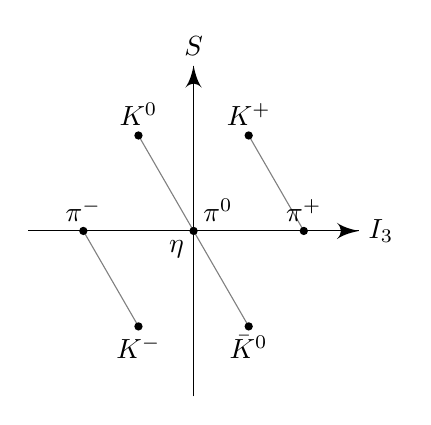
\begin{tikzpicture}[scale=0.7]
    \draw [gray] (-2, 0) -- (-1, -1.732);
    \draw [gray] (2, 0) -- (1, 1.732);
    \draw [gray] (1, -1.732) -- (-1, 1.732);

    \draw [->] (-3, 0) -- (3, 0) node [right] {$I_3$};
    \draw [->] (0, -3) -- (0, 3) node [above] {$S$};
    \node [circ] at (2, 0) {};
    \node [above] at (2, 0) {$\pi^+$};
    \node [circ] at (1, 1.732) {};
    \node [above] at (1, 1.732) {$K^+$};
    \node [circ] at (1, -1.732) {};
    \node [below] at (1, -1.732) {$\bar{K}^0$};
    \node [circ] at (-2, 0) {};
    \node [above] at (-2, 0) {$\pi^-$};
    \node [circ] at (-1, 1.732) {};
    \node [above] at (-1, 1.732) {$K^0$};
    \node [circ] at (-1, -1.732) {};
    \node [below] at (-1, -1.732) {$K^-$};
    \node [circ] at (0, 0) {};
    \node [anchor = north east] at (0, 0) {$\eta$};
    \node [anchor = south west] at (0, 0) {$\pi^0$};
  \end{tikzpicture}
\end{center}

Remarkably, the diagonal lines join together particles of the same charge! Something must be going on here. It turns out if we include these ``strange'' particles into the picture, then instead of a representation of $\su(2)$, we now have representations of $\su(3)$. Indeed, this just looks like a weight diagram of $\su(3)$.

Ultimately, we figured that things are made out of quarks. We now know that there are $6$ quarks, but that's too many for us to handle. The last three quarks are very heavy. They weren't very good at forming hadrons, and their large mass means the particles they form no longer ``look alike''. So we only focus on the first three.

At first, we only discovered things made up of up quarks and down quarks. We can think of these quarks as living in the fundamental representation $V_1$ of $\su(2)$, with
\[
  u =
  \begin{pmatrix}
    1 \\ 0
  \end{pmatrix},\quad
  d =
  \begin{pmatrix}
    0 \\ 1
  \end{pmatrix}.
\]
These are eigenvectors of the Cartan generator $H$, with weights $+\frac{1}{2}$ and $-\frac{1}{2}$ (using the ``physicist's'' way of numbering). The idea is that physics is approximately invariant under the action of $\su(2)$ that mixes $u$ and $d$. Thus, different hadrons made out of $u$ and $d$ might look alike. Nowadays, we know that the QCD part of the Lagrangian is exactly invariant under the $\SU(2)$ action, while the other parts are not.

The anti-quarks lived in the anti-fundamental representation (which is also the fundamental representation). A meson is made of two quarks. So they live in the tensor product
\[
  V_1 \otimes V_1 = V_0 \oplus V_2.
\]
The $V_2$ was the pions we found previously. Similarly, the protons and neutrons consist of three quarks, and live in
\[
  V_1 \otimes V_1 \otimes V_1 = (V_0 \oplus V_2) \otimes V_1 = V_1 \oplus V_1 \oplus V_3.
\]
One of the $V_1$'s contains the protons and neutrons.

The ``strange'' hadrons contain what is known as the strange quark, $s$. This is significantly more massive than the $u$ and $d$ quarks, but are not \emph{too} far off, so we still get a reasonable approximate symmetry. This time, we have three quarks, and they fall into an $\su(3)$ representation,
\[
  u =
  \begin{pmatrix}
    1 \\ 0 \\ 0
  \end{pmatrix},\quad
  d =
  \begin{pmatrix}
    0 \\ 1 \\ 0
  \end{pmatrix},\quad
  s =
  \begin{pmatrix}
    0 \\ 0 \\ 1
  \end{pmatrix}.
\]
This is the fundamental $\mathbf{3}$ representation, while the anti-quarks live in the anti-fundamental $\bar{\mathbf{3}}$. These decompose as
\begin{align*}
  \mathbf{3} \otimes \bar{\mathbf{3}} &= \mathbf{1} \oplus \bar{\mathbf{8}}\\
  \mathbf{3} \otimes \mathbf{3} \otimes \mathbf{3} &= \mathbf{1} \oplus \mathbf{8} \oplus \mathbf{8} \oplus \mathbf{10}.
\end{align*}
The quantum numbers correspond to the weights of the eigenvectors, and hence when we plot the particles according to quantum numbers, they fall in such a nice lattice.

There are a few mysteries left to solve. Experimentally, we found a baryon $\Delta^{++} = uuu$ with spin $\frac{3}{2}$. The wavefunction appears to be symmetric, but this would violate Fermi statistics. This caused theorists to go and scratch their heads again and see what they can do to understand this. Also, we couldn't explain why we only had particles coming from $\mathbf{3} \otimes \bar{\mathbf{3}}$ and $\mathbf{3} \otimes \mathbf{3} \otimes \mathbf{3}$, and nothing else.

The resolution is that we need an extra quantum number. This quantum number is called \term{colour}. This resolved the problem of Fermi statistics, but also, we postulated that any bound state must have no ``net colour''. Effectively, this meant we needed to have groups of three quarks or three anti-quarks, or a quark-antiquark pair. This leads to the idea of \term{confinement}. This principle predicted the $\Omega^-$ baryon $sss$ with spin $\frac{3}{2}$, and was subsequently observed.

Nowadays, we understand this is all due to a $\SU(3)$ gauge symmetry, which is \emph{not} the $\SU(3)$ we encountered just now. This is what we are going to study in this chapter.

\subsection{QCD Lagrangian}
The modern description of the strong interaction of quarks is \term{quantum chromodynamics}, \term{QCD}. This is a gauge theory with a $\SU(3)_C$ gauge group. The strong force is mediated by gauge bosons known as \term{gluons}. This gauge symmetry is exact, and the gluons are massless.

In QCD, each flavour of quark comes in three ``copies'' of different colour. It is conventional to call these colours red, green and blue, even though they have nothing to do with actual colours. For a flavour $f$, we can write these as $q_f^{\mathrm{\color{red} red}}$, $q_f^{\mathrm{\color{mgreen} green}}$ and $q_f^{\mathrm{\color{blue} blue}}$. We can put these into an triplet:
\[
  q_f =
  \begin{pmatrix}
    q_f^{\mathrm{\color{red} red}}\\
    q_f^{\mathrm{\color{mgreen} green}}\\
    q_f^{\mathrm{\color{blue} blue}}
  \end{pmatrix}.
\]
Then QCD says this has an $\SU(3)$ gauge symmetry, where the triplet transforms under the fundamental representation. Since this symmetry is exact, quarks of all three colours behave exactly the same, and except when we are actually doing QCD, it doesn't matter that there are three flavours.

We do this for each quark individually, and then the QCD Lagrangian is given by
\[
  \mathcal{L}_{QCD} = -\frac{1}{4} F^{a\mu\nu} F^a_{\mu\nu} + \sum_f \bar{q}_f (i \slashed{\D} - m_f) q_f,
\]
where, as usual,
\begin{align*}
  \D_\mu &= \partial_\mu + i g A_\mu^a T^a\\
  F_{\mu\nu}^a &= \partial_\mu A_\nu^a - \partial_\nu A_\mu^a - g f^{abc} A_\mu^b A_\nu^c.
\end{align*}
Here $T^a$ for $a = 1, \cdots, 8$ are generators of $\su(3)$, and, as usual, satisfies
\[
  [T^a, T^b] = i f^{abc}T^c.
\]
One possible choice of generators is
\[
  T^a = \frac{1}{2} \lambda^a,
\]
where the $\lambda^a$ are the \term{Gell-Mann matrices}. The fact that we have 8 independent generators means we have 8 gluons.

One thing that is very different about QCD is that it has interactions between gauge bosons. If we expand the Lagrangian, and think about the tree level interactions that take place, we naturally have interactions that look like
\begin{center}
  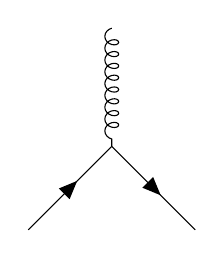
\begin{tikzpicture}
    \begin{feynman}
      \vertex (c);
      \vertex [below left=of c] (bl);
      \vertex [below right=of c] (br);
      \vertex [above=of c] (t);

      \diagram*{
        (bl) -- [fermion] (c) -- [fermion] (br),
        (t) -- [gluon] (c),
      };
    \end{feynman}
  \end{tikzpicture}
\end{center}
but we also have three and four-gluon interactions
\begin{center}
  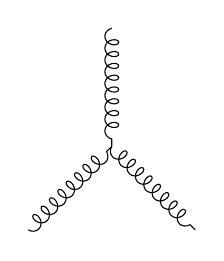
\begin{tikzpicture}
    \begin{feynman}
      \vertex (c);
      \vertex [below left=of c] (bl);
      \vertex [below right=of c] (br);
      \vertex [above=of c] (t);

      \diagram*{
        (bl) -- [gluon] (c) -- [gluon] (br),
        (t) -- [gluon] (c),
      };
    \end{feynman}
  \end{tikzpicture}
  \quad
  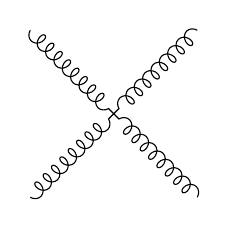
\begin{tikzpicture}
    \begin{feynman}
      \vertex (c);
      \vertex [above right=of c] (1);
      \vertex [above left=of c] (2);
      \vertex [below right=of c] (3);
      \vertex [below left=of c] (4);
      \diagram* {
        (1) -- [gluon] (c),
        (2) -- [gluon] (c),
        (3) -- [gluon] (c),
        (4) -- [gluon] (c),
      };
    \end{feynman}
  \end{tikzpicture}
\end{center}
Mathematically, this is due to the non-abelian nature of $\SU(2)$, and physically, we can think of this as saying the gluon themselves have colour charge.

\subsection{Renormalization}
We now spend some time talking about renormalization of QCD. We didn't talk about renormalization when we did electroweak theory, because the effect is much less pronounced in that case. Renormalization is treated much more thoroughly in the Advanced Quantum Field Theory course, as well as Statistical Field Theory. Thus, we will just briefly mention the key ideas and results for QCD.

QCD has a coupling constant, which we shall call $g$. The idea of renormalization is that this coupling constant should depend on the energy scale $\mu$ we are working with. We write this as $g(\mu)$. However, this dependence on $\mu$ is not arbitrary. The physics we obtain should not depend on the renormalization point $\mu$ we chose. This imposes some restrictions on how $g(\mu)$ depends on $\mu$, and this allows us to define and compute the quantity.
\[
  \beta(g(\mu)) = \mu \frac{\d}{\d \mu} g(\mu).
\]
%
%A theory has a Lagrangian $\mathcal{L}$ that contains a set of couplings $g_i$, which for convenience we take to include the masses. For each of these, we need a physical/observed/derived quantity $g_i^0$ and an expression (renormalization condition)
%\[
% g_i^0 = G_i^0 (\{g_j(\mu)\}, \mu),
%\]
%where $\{g_j(\mu)\} \equiv g(\mu)$ are called \emph{renormalized couplings}, and $\mu$ is the \term{renormalization point}.
%
%We are going to consider perturbative expressions for $G_i^0$.
%
%The physics should not depend on the renormalization point $\mu$, and this tells us how $g(\mu)$ should vary with $\mu$. We define
%\[
% \beta_j(g(\mu), \mu) = \mu \frac{\d}{\d \mu} g_j(\mu).
%\]
%We want $g_i^0$ not to depend on $\mu$. So we get
%\[
% 0 = i \mu \frac{\d}{\d \mu} G_i^0(g(\mu), \mu) = \left(\mu \frac{\partial}{\partial \mu} + \beta_j \frac{\partial}{\partial g_j}\right) G_i^0(g_j(\mu), \mu).
%\]

The $\beta$-function for non-abelian gauge theories typically looks like
\[
  \beta(g) = - \frac{\beta_0 g^3}{16 \pi^2} + O(g^5)
\]
for some $\beta$. For an $\SU(N)$ gauge theory coupled to fermions $\{f\}$ (both left- and right-handed), up to one-loop order,we have
\[
  \beta_0 = \frac{11}{3}N - \frac{4}{3} \sum_f T_f,
\]
where $T_f$ is the \term{Dynkin index} of the representations of the fermion $f$. For the fundamental representation, which is all we are going to care about, we have $T_f = \frac{1}{2}$.
%If $t_f^a$ are the generators of the representations, then the Dynkin index is defined by
%\[
% \Tr (t_f^a t_f^b) = T_f \delta^{ab}. % what actually is this?
%\]
%We assume that the left-handed and right-handed fermions couple equally. For the fundamental representation, we have $T_f = \frac{1}{2}$.
%
%The 1-loop expression for QCD is given by
%\[
% \beta_0 = 11 - \frac{2}{3} n_f,
%\]
%where $n_f$ is the number of quark flavours.

In our model of QCD, we have $6$ quarks. So
\[
  \beta_0 = 11 - 4 = 7.
\]
So we find that the $\beta$-function is always negative!

This isn't actually quite it. The number of ``active'' quarks depends on the energy scale. At energies $\ll m_{\mathrm{top}} \approx \SI{173}{\giga\electronvolt}$, then the top quark is no longer active, and $n_f = 5$. At energies $\sim \SI{100}{\mega\electronvolt}$, we are left with three quarks, and then $n_f = 3$. Matching the $\beta$ functions between these regimes requires a bit of care, and we will not go into that. But in any case, the $\beta$ function is always negative.

Often, we are not interested in the constant $g$ itself, but the \term{strong coupling}
\[
  \alpha_S = \frac{g^2}{4\pi}.
\]
It is an easy application of the chain rule to find that, to lowest order,
\[
  \mu \frac{\d \alpha_S}{\d \mu} = - \frac{\beta_0}{2\pi} \alpha_S^2.
\]
We now integrate this equation, and see what we get. We have
\[
  \int_{\alpha_S(\mu_0)}^{\alpha_S(\mu)} \frac{\d \alpha_S}{\alpha_S^2} = - \frac{\beta_0}{2\pi} \int_{\mu_0}^\mu \frac{\d \mu}{\mu}.
\]
So we find
\[
  \alpha_S(\mu) = \frac{2\pi}{\beta_0} \frac{1}{\log (\mu/\mu_0) + \frac{2\pi}{\beta_0 \alpha_S(\mu_0)}}.
\]
There is an energy scale where $\alpha_S$ diverges, which we shall call $\Lambda_{QCD}$. This is given by
\[
  \log \Lambda_{\mathrm{QCD}} = \log \mu_0 - \frac{2\pi}{\beta_0 \alpha_S(\mu_0)}.
\]
In terms of $\Lambda_{\mathrm{QCD}}$, we can write $\alpha_S(\mu)$ as
\[
  \alpha_S(\mu) = \frac{2\pi}{\beta_0 \log (\mu/\Lambda_{\mathrm{QCD}})}.
\]
Note that in the way we defined it, $\beta_0$ is positive. So we see that $\alpha_S$ \emph{decreases} with increasing $\mu$. This is called \term{asymptotic freedom}. Thus, the divergence occurs at low $\mu$. This is rather different from, say, QED, which is the other way round.

Another important point to get out is that we haven't included any mass term yet, and so we do not have a natural ``energy scale'' given by the masses. Thus, $\mathcal{L}_{\mathrm{QCD}}$ is scale invariant, but quantization has led to a characteristic scale $\Lambda_{\mathrm{QCD}}$. This is called \term{dimensional transmutation}.

What is this scale? This depends on what regularization and renormalization scheme we are using, and tends to be
\[
  \Lambda_{\mathrm{QCD}} \sim 200\mdash 500\SI{}{\mega\electronvolt}.
\]
We can think of this as approximately the scale of the border between perturbative and non-perturbative physics. Note that non-perturbative means we are in low energies, because that is when the coupling is strong!

Of course, we have to be careful, because these results were obtained by only looking up to one-loop, and so we cannot expect it to make sense at low energy scales.

\subsection{\tph{$e^+ e^- \to $ hadrons}{e+e- -> hadrons}{e<sup>+</sup>e<sup>-</sup> &rarr; hadrons}}
Doing QCD computations is very hard\textsuperscript{TM}. Partly, this is due to the problem of confinement. Confinement in QCD means it is impossible to observe free quarks. When we collide quarks together, we can potentially produce single quarks or anti-quarks. Then because of confinement, jets of quarks, anti-quarks and gluons would be produced and combine to form colour-singlet states. This process is known as \term{hadronization}.

Confinement and hadronization are not very well understood, and these happen in the non-perturbative regime of QCD. We will not attempt to try to understand it. Thus, to do computations, we will first \emph{ignore} hadronization, which admittedly isn't a very good idea. We then try to parametrize the hadronization part, and then see if we can go anywhere.

Practically, our experiments often happen at very high energy scales. At these energy scales, $\alpha_S$ is small, and we can expect perturbation theory to work.

We now begin by ignoring hadronization, and try to compute the amplitudes for the interaction
\[
  e^+ e^- \to q\bar{q}.
\]
The leading process is
\begin{center}
  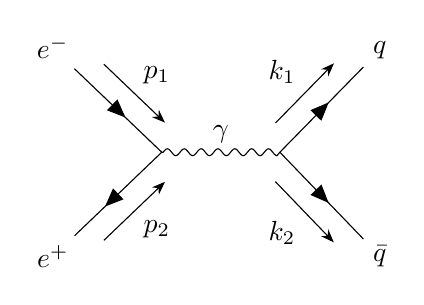
\begin{tikzpicture}
    \begin{feynman}
      \vertex (m1);
      \vertex [above left=of m1] (i1) {$e^-$};
      \vertex [below left=of m1] (i2) {$e^+$};
      \vertex [right=of m1] (m2);
      \vertex [above right=of m2] (f1) {$q$};
      \vertex [below right=of m2] (f2) {$\bar{q}$};

      \diagram*{
        (i1) -- [fermion, momentum=$p_1$] (m1),
        (i2) -- [anti fermion, momentum'=$p_2$] (m1),
        (m2) -- [fermion, momentum'=$k_2$] (f2),
        (m2) -- [fermion, momentum=$k_1$] (f1),
        (m1) -- [photon, edge label=$\gamma$] (m2),
      };
    \end{feynman}
  \end{tikzpicture}
\end{center}
We let
\[
  q = k_1 + k_2 = p_1 + p_2,
\]
and $Q$ be the quark charge. Repeating computations as before, and neglecting fermion masses, we find that
\[
  M = (-ie)^2 Q \bar{u}_q(k_1) \gamma^\mu v_q(k_2) \frac{-ig_{\mu\nu}}{q^2} \bar{v}_e (p_2) \gamma^\nu u_e(p_1).
\]
We average over initial spins and sum over final states. Then we have
\begin{align*}
  \frac{1}{4} \sum_{\mathrm{spins}} |M|^2 &= \frac{e^4 Q^2}{4 q^4} \Tr(\slashed{k}_1 \gamma^\mu \slashed{k}_2 \gamma^\nu) \Tr(\slashed{p}_1 \gamma_\mu \slashed{p}_2 \gamma_\nu)\\
  &= \frac{8 e^4 Q^2}{q^4} \Big((p_1 \cdot k_1) (p_2 \cdot k_2) + (p_1 \cdot k_2) (p_2 \cdot k_1)\Big)\\
  &= e^4 Q^2 (1 + \cos^2 \theta),
\end{align*}
where $\theta$ is the angle between $\mathbf{k}_1$ and $\mathbf{p}_1$, and we are working in the COM frame of the $e^+$ and $e^-$.

Now what we actually want to do is to work out the cross section. We have
\[
  \d \sigma = \frac{1}{|\mathbf{v}_1 - \mathbf{v}_2|} \frac{1}{4 p_1^0 p_2^0} \frac{\d^3 k_1}{ (2\pi)^3 2 k_1^0} \frac{\d^3 k_2}{(2\pi)^3 2 k_2^0} (2\pi)^4 \delta^{(4)} (q - k_1 - k_2) \times \frac{1}{4}\sum_{\mathrm{spins}} |M|^2.
\]
We first take care of the $|\mathbf{v}_1 - \mathbf{v}_2|$ factor. Since $m = 0$ in our approximation, they travel at the speed of light, and we have $|\mathbf{v}_1 - \mathbf{v}_2| = 2$. Also, we note that $k_1^0 = k_2^0 \equiv |\mathbf{k}|$ due to working in the center of mass frame.

Using these, and plugging in our expression for $|M|$, we have
\[
  \d \sigma = \frac{e^4 Q^2}{2} \cdot \frac{1}{16} \cdot \frac{\d^3 k_1 \d^3 k_2}{(2\pi)^2|\mathbf{k}|^4} \delta^{(4)} (q - k_1 - k_2) (1 + \cos^2\theta).
\]
This is all, officially, inside an integral, and if we are only interested in what directions things fly out, we can integrate over the momentum part. We let $\d \Omega$ denote the solid angle, and then
\[
  \d^3 k_1 = |\mathbf{k}|^2 \;\d |\mathbf{k}|\;\d \Omega.
\]
Then, integrating out some delta functions, we obtain
\begin{align*}
  \frac{\d \sigma}{\d \Omega} &= \int \d|\mathbf{k}| \frac{e^4 Q^2}{8 \pi^2 q^4} \frac{1}{2} \delta\left(\frac{\sqrt{q^2}}{2} - |\mathbf{k}|\right)(1 + \cos^2 \theta)\\
  &= \frac{\alpha^2 Q^2}{4 q^2} (1 + \cos^2 \theta),
\end{align*}
where, as usual
\[
  \alpha = \frac{e^2}{4\pi}.
\]
We can integrate over all solid angle to obtain
\[
  \sigma(e^+ e^- \to q \bar{q}) = \frac{4\pi \alpha^2}{3 q^2}Q^2.
\]
We can compare this to $e^+ e^- \to \mu^+ \mu^-$, which is exactly the same, except we put $Q = 1$ because that's the charge of a muon.

But this isn't it. We want to include the effects of hadronization. Thus, we want to consider the decay of $e^+ e^-$ into any possible hadronic final state. For any final state $X$, the invariant amplitude is given by
\[
  M_X = \frac{e^2}{q^2} \brak{X} J^\mu_h \bket{0} \bar{v}_e (p_2) \gamma^\nu u_e(p_1),
\]
where
\[
  J^\mu_h = \sum_f Q_f \bar{q}_f \gamma^\mu q_f,
\]
and $Q_f$ is the quark charge. Then the total cross section is
\[
  \sigma(e^+ e^- \to \mathrm{hadrons}) = \frac{1}{8p_1^0 p_2^0} \sum_{X} \frac{1}{4} \sum_{\mathrm{spins}} (2\pi)^4 \delta^{(4)} (q - p_X) |M_X|^2.
\]
We can't compute perturbatively the hadronic bit, because it is non-perturbative physics. So we are going to parameterize it in some way. We introduce a \term{hadronic spectral density}\index{$\rho_h^{\mu\nu}(q)$}
\[
  \rho_h^{\mu\nu} (q) = (2\pi)^3 \sum_{X, p_X} \delta^{(4)} (q - p_X) \brak{0}J_h^\mu\bket{X} \brak{X}J_h^\nu\bket{0}.
\]
We now do some dodgy maths. By current conservation, we have $q_\mu \rho^{\mu\nu} = 0$. Also, we know $X$ has positive energy. Then Lorentz covariance forces $\rho_h$ to take the form
\[
  \rho_h^{\mu\nu}(q) = (- g^{\mu\nu} q^2 + q^\mu q^\nu) \Theta(q^0) \rho_h (q^2).
\]
We can then plug this into the cross-section formula, and doing annoying computations, we find
\begin{align*}
  \sigma &= \frac{1}{8 p_1^0 p_2^0} \frac{(2\pi) e^4}{4 q^4} 4 (p_{1\mu} p_{2\nu} - p_1 \cdot p_2 g_{\mu\nu} + p_{1\nu} p_{2\mu})(-g^{\mu\nu} q^2 + q^\mu q^\nu) \rho_h(q^2)\\
  &= \frac{16 \pi^3 \alpha^2}{q^2} \rho_h(q^2).
\end{align*}
Of course, we can't compute this $\rho_h$ directly. However, if we are lazy, we can consider only quark-antiquark final states $X$. It turns out this is a reasonably good approximation. Then we obtain something similar to what we had at the beginning of the section. We will be less lazy and include the quark masses this time. Then we have
%
%
%We might think this is all we can do. But if we make a further assumption, then we can go a bit further. We assume
%\[
% \sum_{X \in \mathrm{Had}}\bket{X}\brak{X} = \sum_{X \in q, \bar{q}, g\text{ states}} \bket{X}\brak{X}.
%\]
%This is known as \term{quark-hadron duality}. This is not proved to be valid, but works reasonably well. The assumption we are making is that $e^+ e^- \to \gamma^* \to q\bar{q}$ can be separated from hadronization. If we make this assumption, then we can actually write down the value of $\rho_h$. We have
\begin{multline*}
  \rho_h^{\mu\nu}(q^2) = N_c \sum_f Q_f^2 \int \frac{\d^3 k_1}{(2\pi)^3 2 k_1^0} \int \frac{\d^3 k_2}{(2\pi)^3 2k_2^0} (2\pi)^3 \delta^{(4)}(q - k_1 - k_2)\\
  \times \left.\Tr [(\slashed{k}_1 + m_f) \gamma^\mu (\slashed{k}_2 - m_f) \gamma^{\nu}]\right|_{k_1^2 = k_2^2 = m_f^2}, % what does this mean?
\end{multline*}
where $N_c$ is the number of colours and $m_f$ is the quark $q_f$ mass. We consider the quantity
\[
  I^{\mu\nu} = \left.\int \frac{\d^3 k_1}{k_1^0} \int \frac{\d^3 k_2}{k_2^0} \delta^{(4)}(q - k_1 - k_2) k_1^\mu k_2^\nu\right|_{k_1^2 = k_2^2 = m_f^2}.
\]
We can argue that we can write
\[
  I^{\mu\nu} = A(q^2) q^\mu q^\nu + B(q^2) g^{\mu\nu}.
\]
We contract this with $g_{\mu\nu}$ and $q_\mu q_\nu$ (separately) to obtain equations for $A, B$. We also use
\[
  q^2 = (k_1 + k_2)^2 = 2 m_f^2 + 2 k_1 \cdot k_2.
\]
We then find that
\[
  \rho_h(q^2) = \frac{N_c}{12 \pi^2} \sum_f Q_f^2 \Theta(q^2 - 4 m_f^2)\left(1 - \frac{4 m_f^2}{q^2}\right)^{1/2} \frac{q^2 + 2 m_f^2}{q^2}.
\]
That's it! We can now plug this into the equation we had for the cross-section. It's still rather messy. If all $m_f \to 0$, then this simplifies very nicely, and we find that
\[
  \rho_h(q^2) = \frac{N_c}{12 \pi^2} \sum_f Q_f^2.
\]
Then after some hard work, we find that
\[
  \sigma_{\mathrm{LO}}(e^+ e^- \to \mathrm{hadrons}) = N_c \frac{4\pi \alpha^2}{3q^2} \sum_f Q_f^2,
\]
where LO denotes ``leading order''.

An experimentally interesting quantity is the following ratio:
\[
  R = \frac{\sigma(e^+ e^- \to \mathrm{hadrons})}{\sigma(e^+ e^- \to \mu^+ \mu^-)}.
\]
Then we find that
\[
  R_{LO} = N_c \sum_f Q_f^2 =
  \begin{cases}
    \frac{2}{3} N_c & \text{when $u$, $d$, $s$ are active}\\
    \frac{10}{9} N_c & \text{when $u$, $d$, $s$, $c$ are active}\\
    \frac{11}{9} N_c & \text{when $u$, $d$, $s$, $c$, $b$ are active}
  \end{cases}
\]
In particular, we expect ``jumps'' as we go between the quark masses. Of course, it is not going to be a sharp jump, but some continuous transition.

We've been working with tree level diagrams so far. The one-loop diagrams are UV finite but have IR divergences, where the loop momenta $\to 0$. The diagrams include
\begin{center}
  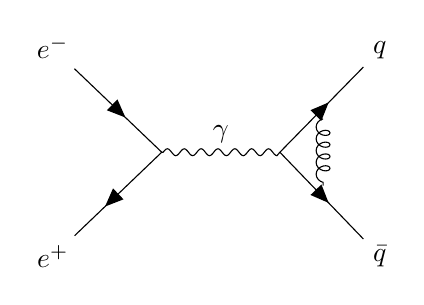
\begin{tikzpicture}
    \begin{feynman}
      \vertex (m1);
      \vertex [above left=of m1] (i1) {$e^-$};
      \vertex [below left=of m1] (i2) {$e^+$};
      \vertex [right=of m1] (m2);
      \vertex [above right=of m2] (f1) {$q$};
      \vertex [below right=of m2] (f2) {$\bar{q}$};

      \vertex [above right=0.6cm of m2] (g1) {};
      \vertex [below right=0.6cm of m2] (g2) {};
      \diagram*{
        (i1) -- [fermion] (m1),
        (i2) -- [anti fermion] (m1),
        (m2) -- [fermion] (f2),
        (m2) -- [fermion] (f1),
        (m1) -- [photon, edge label=$\gamma$] (m2),
        (g1) -- [gluon] (g2),
      };
    \end{feynman}
  \end{tikzpicture}
  \quad
  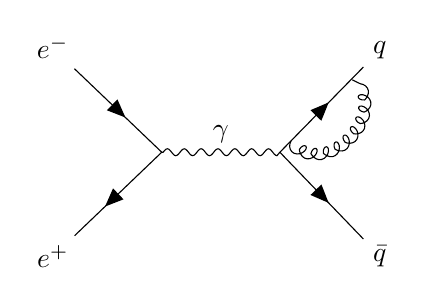
\begin{tikzpicture}
    \begin{feynman}
      \vertex (m1);
      \vertex [above left=of m1] (i1) {$e^-$};
      \vertex [below left=of m1] (i2) {$e^+$};
      \vertex [right=of m1] (m2);
      \vertex [above right=of m2] (f1) {$q$};
      \vertex [below right=of m2] (f2) {$\bar{q}$};

      \vertex [above right=0.2cm of m2] (g1);
      \vertex [above right=1.3cm of m2] (g2);
      \diagram*{
        (i1) -- [fermion] (m1),
        (i2) -- [anti fermion] (m1),
        (m2) -- [fermion] (f2),
        (m2) -- [fermion] (f1),
        (m1) -- [photon, edge label=$\gamma$] (m2),
        (g1) -- [gluon, half right] (g2), % make this move
      };
    \end{feynman}
  \end{tikzpicture}
  \quad
  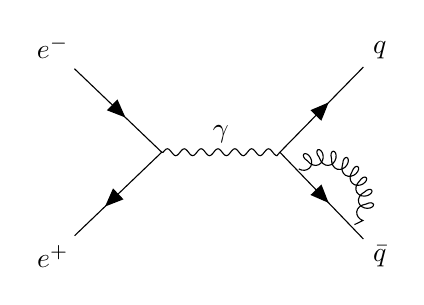
\begin{tikzpicture}
    \begin{feynman}
      \vertex (m1);
      \vertex [above left=of m1] (i1) {$e^-$};
      \vertex [below left=of m1] (i2) {$e^+$};
      \vertex [right=of m1] (m2);
      \vertex [above right=of m2] (f1) {$q$};
      \vertex [below right=of m2] (f2) {$\bar{q}$};

      \vertex [left=0.22cm of m2] (l);

      \vertex [below right=0.3cm of l] (g1) {};
      \vertex [below right=1.3cm of l] (g2) {};
      \diagram*{
        (i1) -- [fermion] (m1),
        (i2) -- [anti fermion] (m1),
        (m2) -- [fermion] (f2),
        (m2) -- [fermion] (f1),
        (m1) -- [photon, edge label=$\gamma$] (m2),
        (g1) -- [gluon, half left] (g2), % make this move
      };
    \end{feynman}
  \end{tikzpicture}
\end{center}
However, it turns out the IR divergence is cancelled by tree level $e^+ e^- \to q\bar{q} g$ such as
\begin{center}
  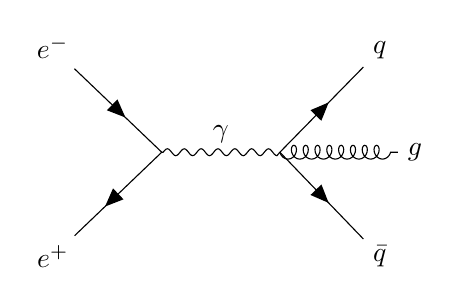
\begin{tikzpicture}
    \begin{feynman}
      \vertex (m1);
      \vertex [above left=of m1] (i1) {$e^-$};
      \vertex [below left=of m1] (i2) {$e^+$};
      \vertex [right=of m1] (m2);
      \vertex [above right=of m2] (f1) {$q$};
      \vertex [below right=of m2] (f2) {$\bar{q}$};

      \vertex [right=of m2] (g2) {$g$};
      \diagram*{
        (i1) -- [fermion] (m1),
        (i2) -- [anti fermion] (m1),
        (m2) -- [fermion] (f2),
        (m2) -- [fermion] (f1),
        (m1) -- [photon, edge label=$\gamma$] (m2),
        (m2) -- [gluon] (g2),
      };
    \end{feynman}
  \end{tikzpicture}
\end{center}
\subsection{Deep inelastic scattering}
In this chapter, we are going to take an electron, accelerate it to really high speeds, and then smash it into a proton.

If we do this at low energies, then the proton appears pointlike. This is Rutherford and Mott scattering we know and love from A-levels Physics. If we increase the energy a bit, then the wavelength of the electron decreases, and now the scattering would be sensitive to charge distributions within the proton. But this is still elastic scattering. After the interactions, the proton remains a proton and the electron remains an electron.

What we are interested in is \emph{inelastic} scattering. At very high energies, what tends to happen is that the proton breaks up into a lot of hadrons $X$. We can depict this interaction as follows:
\begin{center}
  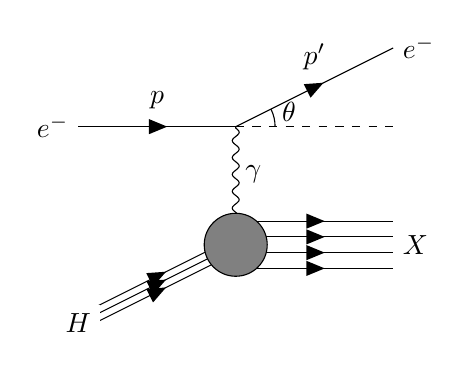
\begin{tikzpicture}
    \draw [/tikzfeynman/fermion] (-2, -1) -- (0, 0);
    \draw [/tikzfeynman/fermion] (-2, -0.9) -- (0, 0.1);
    \draw [/tikzfeynman/fermion] (-2, -1.1) -- (0, -0.1);

    \node [fill=white] (H) at (-2, -1) {$H$};

    \draw [/tikzfeynman/fermion] (0, 0.1) -- +(2, 0);
    \draw [/tikzfeynman/fermion] (0, 0.3) -- +(2, 0);
    \draw [/tikzfeynman/fermion] (0, -0.1) -- +(2, 0);
    \draw [/tikzfeynman/fermion] (0, -0.3) -- +(2, 0);


    \draw [/tikzfeynman/fermion] (-2, 1.5) node [left] {$e^-$} -- (0, 1.5) node [pos=0.5, above=0.1cm] {$p$};
    \draw [/tikzfeynman/fermion] (0, 1.5) -- (2, 2.5) node [right] {$e^-$} node [pos=0.5, above=0.1cm] {$p'$};

    \draw [/tikzfeynman/photon] (0, 1.5) -- (0, 0) node [pos=0.4, right] {$\gamma$};
    \node [right] at (2, 0) {$X$};
    \draw [fill=gray] circle [radius=0.4cm];

    \draw [dashed] (0, 1.5) -- (2, 1.5);

    \draw (0.5, 1.5) arc(0:26.565:0.5) node [pos=0.8, right] {$\theta$};

  \end{tikzpicture}
\end{center}

This led to the idea that hadrons are made up of \term{partons}. When we first studied this, we thought these partons are weakly interacting, but nowadays, we know this is due to asymptotic freedom.

Let's try to understand this scattering. The final state $X$ can be very complicated in general, and we have no interest in this part. We are mostly interested in the difference in momentum,
\[
  q = p - p',
\]
as well as the scattering angle $\theta$. We will denote the mass of the initial hadron $H$ by $M$, and we shall treat the electron as being massless.

It is conventional to define
\[
  Q^2 \equiv - q^2 = 2 p \cdot p' = 2 E E' (1 - \cos \theta) \geq 0,
\]
where $E = p^0$ and $E' = p'^0$, since we assumed electrons are massless. We also let
\[
  \nu = p_H \cdot q.
\]
It is an easy manipulation to show that $p_X^2 = (p_H + q)^2 \geq M^2$. This implies
\[
  Q^2 \leq 2 \nu.
\]
For simplicity, we are going to consider the scattering in the rest frame of the hadron. In this case, we simply have
\[
  \nu = M(E - E')
\]
We can again compute the amplitude, which is confusingly also called $M$:
\[
  M = (ie)^2 \bar{u}_e (p') \gamma^\mu u_e (p) \left(-\frac{i g_{\mu\nu}}{q^2} \brak{X} J_h^\nu \bket{H(p_H)}\right).
\]
Then we can write down the differential cross-section
\[
  \d \sigma = \frac{1}{4 ME |\mathbf{v}_e - \mathbf{v}_H|} \frac{\d^3 p'}{(2\pi)^3 2 p'^0} \sum_{X, p_X} (2\pi)^4 \delta^{(4)} (q + p_H - p_X) \frac{1}{2} \sum_{\mathrm{spins}} |M|^2.
\]
Note that in the rest frame of the hadron, we simply have $|\mathbf{v}_e - \mathbf{v}_H| = 1$.

We can't actually compute this non-perturbatively. So we again have to parametrize this. We can write
\[
  \frac{1}{2} \sum_{\mathrm{spins}} |M|^2 = \frac{e^4}{2q^4} L_{\mu\nu} \brak{H(p_H)} J_h^\mu \bket{X} \brak{X} J^\nu_h\bket{H(p_H)},
\]
where
\[
  L_{\mu\nu} = \Tr \left(\slashed{p} \gamma^\mu \slashed{p}' \gamma^\nu) = 4(p_\mu p'_\nu - g_{\mu\nu} p \cdot p' + p_\nu p_\mu'\right).
\]
We define another tensor
\[
  W^{\mu\nu}_H = \frac{1}{4\pi} \sum_X (2\pi)^4 \delta^{(4)} (p + p_H - o_X) \brak{H}J_h^\mu \bket{X} \brak{X} J_H^\nu \bket{H}.
\]
Note that this $\sum_X$ should also include the sum over the initial state spins. Then we have
\[
  E' \frac{\d \sigma}{\d^3 p'} = \frac{1}{8ME(2\pi)^3} 4\pi \frac{e^4}{2q^4} L_{\mu\nu} W^{\mu\nu}_H.
\]
We now use our constraints on $W^{\mu\nu}_H$ such as Lorentz covariance, current conservation and parity, and argue that $W^{\mu\nu}_H$ can be written in the form
\begin{multline*}
  W_H^{\mu\nu} = \left(- g^{\mu\nu} + \frac{q^\mu q^\nu}{q^2}\right) W_1(\nu, Q^2) \\
  + \left(p_H^\mu - \frac{p_H \cdot q}{q^2} q^\mu\right) \left(p_H^\nu - \frac{p_H \cdot q}{q^2}q^\nu\right) \times W_2(\nu, Q^2).
\end{multline*}
Now, using
\[
  q^\mu L_{\mu\nu} = q^\nu L_{\mu\nu} = 0,
\]
we have
\begin{align*}
  L_{\mu\nu} W_H^{\mu\nu} &= 4 (-2 p\cdot p' + 4 p\cdot p') W_1 + 4(2 p\cdot p_H p'\cdot p_H - p_H^2 p \cdot p')\\
  &= 4Q^2 W_1 + 2M^2 (4 EE' - Q^2)W_2.
\end{align*}
We now want to examine what happens as we take the energy $E \to \infty$. In this case, for a generic collision, we have $Q^2 \to \infty$, which necessarily implies $\nu \to \infty$. To understand how this behaves, it is helpful to introduce dimensionless quantities
\[
  x = \frac{Q^2}{2 \nu},\quad y = \frac{\nu}{p_H \cdot p},
\]
known as the \term{Bjorken $x$} and the \term{inelasticity} respectively. We can interpret $y$ as the fractional energy loss of the electron. Then it is not difficult to see that $0 \leq x, y \leq 1$. So these are indeed bounded quantities. In the rest frame of the hadron, we further have
\[
  y = \frac{\nu}{ME} = \frac{E - E'}{E}.
\]
This allows us to write $L_{\mu\nu}W_H^{\mu\nu}$ as
\[
  L_{\mu\nu} W^{\mu\nu}_H \approx 8EM \left(xy W_1 + \frac{(1 - y)}{y} \nu W_2\right),
\]
where we dropped the $-2M^2Q^2 W_2$ term, which is of lower order.

To understand the cross section, we need to simplify $\d^3 p'$. We integrate out the angular $\phi$ coordinate to obtain
\[
  \d^3 p' \mapsto 2\pi E'^2 \;\d (\cos \theta)\;\d E'.
\]
We also note that by definition of $Q, x, y$, we have
\begin{align*}
  \d x &= \d \left(\frac{Q^2}{2\nu}\right) = - 2EE' \;\d \cos \theta + (\cdots)\;\d E'\\
  \d y &= -\frac{\d E'}{E}.
\end{align*}
Since $(\d E')^2 = 0$, the $\d^3 p'$ part becomes
\[
  \d^3 p' \mapsto \pi E'\;\d Q^2\;\d y = 2\pi E' \nu\;\d x\;\d y.
\]
Then we have
\begin{align*}
  \frac{\d \sigma}{\d x\; \d y} &= \frac{1}{8(2\pi)^2} \frac{1}{EM} \frac{e^4}{q^4} 2\pi \nu \cdot 8EM\left(xy W_1 + \frac{(1 - y)}{y} \nu W_2\right)\\
  &= \frac{8 \pi \alpha^2 ME}{Q^4}\left( xy^2 F_1 + (1 - y) F_2\right),
\end{align*}
where
\[
  F_1 \equiv W_2,\quad F_2 \equiv \nu W_2.
\]
By varying $x$ and $y$ in experiments, we can figure out the values of $F_1$ and $F_2$. Moreover, we expect if we do other sorts of experiments that also involve hadrons, then the same $F_1$ and $F_2$ will appear. So if we do other sorts of experiments and measure the same $F_1$ and $F_2$, we can increase our confidence that our theory is correct.

Without doing more experiments, can we try to figure out something about $F_1$ and $F_2$? We make a simplifying assumption that the electron interacts with only a single constituent of the hadron:
\begin{center}
  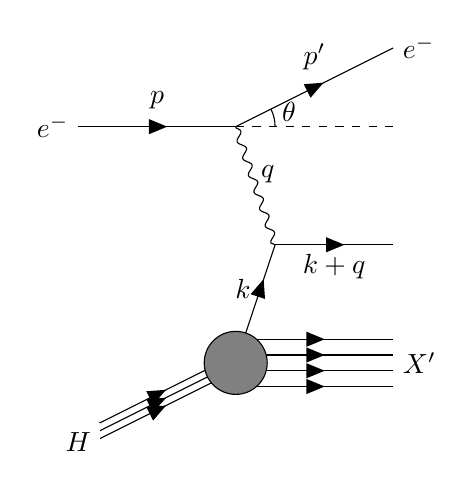
\begin{tikzpicture}
    \draw [/tikzfeynman/fermion] (-2, -1) -- (0, 0);
    \draw [/tikzfeynman/fermion] (-2, -0.9) -- (0, 0.1);
    \draw [/tikzfeynman/fermion] (-2, -1.1) -- (0, -0.1);

    \node [fill=white] (H) at (-2, -1) {$H$};

    \draw [/tikzfeynman/fermion] (0, 0.1) -- +(2, 0);
    \draw [/tikzfeynman/fermion] (0, 0.3) -- +(2, 0);
    \draw [/tikzfeynman/fermion] (0, -0.1) -- +(2, 0);
    \draw [/tikzfeynman/fermion] (0, -0.3) -- +(2, 0);


    \draw [/tikzfeynman/fermion] (-2, 3) node [left] {$e^-$} -- (0, 3) node [pos=0.5, above=0.1cm] {$p$};
    \draw [/tikzfeynman/fermion] (0, 3) -- (2, 4) node [right] {$e^-$} node [pos=0.5, above=0.1cm] {$p'$};

    \draw [/tikzfeynman/photon] (0, 3) -- (0.5, 1.5) node [pos=0.4, right] {$q$};
    \draw [/tikzfeynman/fermion] (0.1265, 0.3795) -- (0.5, 1.5) node [pos=0.5, left] {$k$};
    \draw [/tikzfeynman/fermion] (0.5, 1.5) -- (2, 1.5) node [pos=0.5, below] {$k + q$};

    \node [right] at (2, 0) {$X'$};
    \draw [fill=gray] circle [radius=0.4cm];

    \draw [dashed] (0, 3) -- (2, 3);

    \draw (0.5, 3) arc(0:26.565:0.5) node [pos=0.8, right] {$\theta$};
  \end{tikzpicture}
\end{center}

We further suppose that the EM interaction is unaffected by strong interactions. This is known as \term{factorization}. This leading order model we have constructed is known as the \term{parton model}. This was the model used before we believed in QCD. Nowadays, since we do have QCD, we know these ``partons'' are actually quarks, and we can use QCD to make some more accurate predictions.

We let $f$ range over all partons. Then we can break up the sum $\sum_X$ as
\[
  \sum_X = \sum_{X'} \sum_f \frac{1}{(2\pi)^3} \int \d^4 k\; \Theta(k^0) \delta(k^2) \sum_{\mathrm{spins}},
\]
where we put $\delta(k^2)$ because we assume that partons are massless.

To save time (and avoid unpleasantness), we are not going to go through the details of the calculations. The result is that
\[
  W_H^{\mu\nu} = \sum_f \int \d^4 k \Tr\left(W_f^{\mu\nu} \Gamma_{H, f} (p_H, k) + \bar{W}_f^{\mu\nu} \bar{\Gamma}_{H, f} (p_H, k)\right),
\]
where
\begin{align*}
  W_f^{\mu\nu} &= \bar{W}_f^{\mu\nu} = \frac{1}{2} Q_f^2 \gamma^\mu (\slashed{k} + \slashed{q}) \gamma^\nu \delta((k + q)^2)\\
  \Gamma_{H, f} (p_H, k)_{\beta\alpha} &= \sum_{X'} \delta^{(4)} (p_H - k - p_X') \brak{H(p_H)} \bar{q}_{f, \alpha} \bket{X'} \brak{X'}q_{f, \beta}\bket{H(p_H)},
\end{align*}
where $\alpha, \beta$ are spinor indices.

In the deep inelastic scattering limit, putting everything together, we find
\begin{align*}
  F_1(x, Q^2) &\sim \frac{1}{2} \sum_f Q_f^2 [ q_f(x) + \bar{q}_f(x)]\\
  F_2(x, Q^2) &\sim 2 x F_1,
\end{align*}
for some functions $q_f(x)$, $\bar{q}_f(x)$. These functions are known as the \term{parton distribution functions} (\term{PDF}'s). They are roughly the distribution of partons with the longitudinal momentum function.

The very simple relation between $F_2$ and $F_1$ is called the \term{Callan--Gross relation}, which suggests the partons are spin $\frac{1}{2}$. This relation between $F_2$ and $F_1$ is certainly something we can test in experiments, and indeed they happen. We also see the \term{Bjorken scaling phenomenon} --- $F_1$ and $F_2$ are independent of $Q^2$. This boils down to the fact that we are scattering with point-like particles.

%\section{Effective Field Theory}
%Actual QCD calculations, even at high energies where it is perturbative, are difficult. If we go to the non-perturbative regime, then obviously we can't do perturbative calculations. What can we do?
%
%One possibility is to use numerical methods called \term{lattice field theory}, or in this case, \term{lattice QCD}. Unfortunately, this is not what we are going to talk about, but we can get some insights into what is going on with effective field theories.
%
%In effective field theory, we exploit large separations in energy scale to construct a description of low-energy physics. For example, in Fermi theory, approximated the $W$-boson propagator
%\[
% \frac{1}{p^2 - m_W^2} \approx - \frac{1}{m_W^2} - \frac{p^2}{m_W^4} + \cdots
%\]
%for $p^2 \ll m_W^2$. This is an example of effective field theory.
%% Georgi, Ann. Rev. Nucl. Part. Sci. 43:209 (1903)
%% Kaplan, arXiv nucl-th/0501023 (2005)
%
%We are now going to do this in a more general and formal way.
%\subsection{Scaling dimensions of local operators}
%In principle, we can have an infinite number of term in $\mathcal{L}$, because an effective field theory is only valid up to a scale $\Lambda$, and we have no constraint imposed by renormalization.
%
%Of course, symmetries can still provide constraints. If we want a Lorentz-invariant theory, then we can only write down Lorentz-invariant terms. We write
%\[
% \mathcal{L}_{\mathrm{eff}} = \mathcal{L}_{\mathrm{kin}} + \sum_n \mathcal{L}_{\mathrm{int}}^{(n)},
%\]
%Since the action is dimensionless, we know we must have mass dimension $[\mathcal{L}] = 4$. We write
%\[
% \mathcal{L}_{\mathrm{int}}^{(n + 4)} = \sum \frac{c_i^{(n)}}{\Lambda^n} \mathcal{O}_i^{(n + 4)},
%\]
%where $\Lambda$ is some heavy mass scale independent of $n$, with $[\Lambda] = 1$, $[c_i^{(n)}] = 0$, and $\mathcal{O}^{(n + 4)}$ is an operator of dimension $n + 4$.
%
%For example, in Fermi theory, we can take $\Lambda$ to be the $W$-boson mass.
%
%We assume
%\begin{enumerate}
% \item We have a finite number of independent operators in each fixed mass dimension.
% \item $c_i^{(n)}$ are at most order $1$
%\end{enumerate}
%We can now truncate the series depending on the accuracy we want. Suppose we are working at an energy scale $E$. To obtain an accuracy of accuracy $\sim \varepsilon$, we must find an $n_\varepsilon$ such that
%\[
% \left(\frac{E}{\Lambda}\right)^{n_\varepsilon} \approx \varepsilon.
%\]
%Rearranging, we find
%\[
% n_\varepsilon \approx \frac{\log (1/\varepsilon)}{\log(\Lambda/E)}.
%\]
%So to obtain greater accuracy, we need to look at more terms.
%
%\begin{eg}
% Consider a real scalar field in $4$ dimensions. Assume this has the additional symmetry of $\phi \mapsto -\phi$. We are also going to work in Euclidean spacetime to get around some technical issues.
%
% The constraint of the symmetry means we only have to care about terms with an even number of $\phi$'s. Then we can write
% \[
% \mathcal{L} = \frac{1}{2} (\partial \phi)^2 + \frac{1}{2} m^2 \phi^2 + \frac{\lambda}{4!} \phi^4 + \sum_{n = 1}^\infty\left(\frac{c_n}{\Lambda^{2n}} \phi^{4 + 2n} + \frac{d_n}{\Lambda^{2n}} (\partial \phi)^2 \phi^{2n} + \cdots\right).
% \]
% As before, $[\phi] = 1$ and $\lambda, c_n, d_n$ are dimensionless, and order $1$ or smaller.
%\end{eg}
%
%In general, we are interested in the correlation function
%\[
% \bra \phi_1 \cdots \phi_n\ket = \frac{1}{2} \int \D \phi\; \phi_1 \cdots \phi_n e^{-S},\quad \mathcal{Z} = \int \D \phi\; e^{-S}.
%\]
%Here
%\[
% S = \int \d^x\; \mathcal{L}
%\]
%is the Euclidean action. There are two arguments to justify truncating the sum.
%\begin{enumerate}
% \item Consider a specific field configuration $\tilde{\phi}(x)$ localized in some volume $L^4$, where $L \approx \frac{2\pi}{k}$ with $k$ the wavenumber or momentum. The amplitude of the wavelet is $\phi_k$, and define
% \[
% \hat{\phi}_k = \frac{1}{k} \phi_k.
% \]
% We are going to crudely approximate the terms in $S$. This is
% \[
% \int \d^4 x\; m^2 \tilde{\phi}^2 \approx L^4 m^2 \phi_k^2 = \left(\frac{\pi}{k}\right)^4 m^2 k^2 \hat{\phi}_k^2 = \frac{(2\pi)^4}{k^2} m^2 \hat{\phi}_k.
% \]
% Also, we have
% \[
% \int \d^4 x\; (\partial \tilde{\phi})^2 \approx L^4 k^2 \phi_k^2 = (2\pi)^4 \hat{\phi}_k^2.
% \]
% Then we have
% \[
% \frac{1}{\Lambda^{2p + q - 4}} \int \d^4 x\; (\partial \tilde{\phi})^p \tilde{\phi}^q \approx \frac{L^4 k^{2p} k^q \hat{\phi}_k^{p + q}}{\Lambda^{2p + q - 4}} = (2\pi)^4 \left(\frac{k}{\Lambda}\right)^{2p + q - 4} \hat{\phi}_k^{p + q}.
% \]
% So we have
% \[
% S \approx (2\pi)^4 \left( \frac{1}{2} \hat{\phi}_k^2 + \frac{m^2 \hat{\phi}_k^2}{2k^2} + \frac{\lambda}{4!} \hat{\phi}_k^4 + \sum_{n = 1}^\infty \left(c_n \left(\frac{k}{\Lambda}\right)^{2n} \hat{\phi}_k^{4 + 2n} + d_n \left(\frac{k}{\Lambda}\right)^{2n} \hat{\phi}_k^{2 + 2n} + \cdots\right)\right).
% \]
% Path integrals are dominated by $\hat{\phi}_k$ that minimize $S$. Consider the quadratic terms, for relative scales $k^2 \gg m^2$. So kinetic term dominates and $\hat{\phi}_k \approx \frac{1}{(2\pi)^2}$ or similar.
%
% As $k$ is reduced, $\left(\frac{k}{\Lambda}\right)^{2n}$ terms are reduced. These are called \term{irrelevant terms}. The mass term is a \term{relevant term}, and the $\phi^4$ term is a \term{marginal term}.
%
% \item We can adopt a more general argument using scale transformations. $\phi(x)$ is an arbitrary field configuration, and consider
% \[
% \phi_\xi(x) = \phi(\xi x),\quad x' = \xi x,\quad \phi'(x') = \frac{1}{\xi}\phi(\xi, x).
% \]
% Note that the prime is \emph{not} differentiation. Consider
% \[
% S(\phi_\xi(x), m^2, \lambda, c_n, d_n, \cdots) = S(\xi^{-1}\phi(x), \xi^{-2} m^2, \lambda, \xi^{2n} c_n, \xi^{2n} d_n, \cdots).
% \]
% As $\xi \to 0$, we expose the infrared ``flow'' of the couplings, as
% \[
% \phi(x) \sim e^{+ i k\cdot x},\quad \phi_\xi (x) = e^{i (\xi k) \cdot x}.
% \]
% What we see from this argument again is that these couplings go smaller as we go towards the infrared.
%\end{enumerate}

\printindex%
\end{document}
